\documentclass[12pt,a4paper]{report}
\AtBeginDocument{\fontsize{13}{15.6}\selectfont} % 13pt body; report has no 13pt option
\usepackage[utf8]{inputenc}\usepackage[T5]{fontenc}\usepackage[english,main=vietnamese]{babel}
\usepackage{mathptmx}                       % Times New Roman
\usepackage[top=2cm,bottom=2cm,left=3cm,right=2cm]{geometry}
\usepackage{setspace}\onehalfspacing
\usepackage{graphicx,booktabs,amsmath,longtable,hyperref,caption}
\usepackage{csquotes}
\usepackage[table]{xcolor}
\usepackage[style=apa,backend=biber,language=english,autolang=other,sortlocale=en_US]{biblatex} % biber has no Vietnamese locale
\DeclareLanguageMapping{english}{english-apa}
\addbibresource{references.bib}
% biblatex-apa has no vietnamese-apa.lbx: reuse the English APA strings for Vietnamese text
\DeclareLanguageMapping{vietnamese}{english-apa}
\hypersetup{hidelinks}
\graphicspath{{images/}}
\usepackage{tikz}\usetikzlibrary{arrows.meta,positioning,fit}

\begin{document}
% ---------- Bìa + phụ bìa theo mẫu KL01 (Khoa HTTT, UEL) ----------
% Ảnh nền (khung, logo, dải xanh) trích từ file hướng dẫn .doc của khoa.
\newcommand{\coverpage}{%
\begin{titlepage}
\begin{tikzpicture}[remember picture,overlay]
  \node[inner sep=0] at (current page.center)
    {
\includegraphics[width=\paperwidth,height=\paperheight]{cover-kl01-vi}};
  \node[font=\bfseries\fontsize{16}{20}\selectfont] at ([yshift=-4.6cm]current page.north) {KHOA HỆ THỐNG THÔNG TIN};
  \node[font=\bfseries\fontsize{14}{18}\selectfont] at ([yshift=-11.3cm]current page.north) {KHÓA LUẬN TỐT NGHIỆP};
  \node[font=\bfseries\fontsize{18}{24}\selectfont,text width=16cm,align=center]
    at ([yshift=-13.3cm]current page.north)
    {GIAO ĐÚNG HẠN, VẪN CHƯA HÀI LÒNG\\[4pt]
     {\fontsize{14}{19}\selectfont HỆ THỐNG HỌC MÁY PHÁT HIỆN SỚM VÀ ƯU TIÊN CHĂM SÓC\\
      ĐƠN HÀNG CÓ NGUY CƠ BẤT MÃN ẨN TRÊN DỮ LIỆU OLIST}};
  \node[font=\bfseries\fontsize{13}{18}\selectfont,anchor=north west,align=left]
    at ([xshift=-1.2cm,yshift=-17.3cm]current page.north)
    {GVHD: TODO\\SVTH: TODO\\MSSV: TODO};
  \node[font=\bfseries\fontsize{13}{16}\selectfont,text=white]
    at ([yshift=2.25cm]current page.south) {TP.HCM, THÁNG \,TODO/2026};
\end{tikzpicture}
\end{titlepage}}
\coverpage   % trang bìa

\pagenumbering{roman}
% Thứ tự theo hướng dẫn Khoa HTTT, mục II
\chapter*{Lời cảm ơn}
\chapter*{Lời cam kết}
\tableofcontents
\listoffigures\addcontentsline{toc}{chapter}{Danh mục hình ảnh}
\listoftables\addcontentsline{toc}{chapter}{Danh mục bảng biểu}
\chapter*{Danh mục từ viết tắt}\addcontentsline{toc}{chapter}{Danh mục từ viết tắt}
% TODO: bảng 2 cột (từ viết tắt | nghĩa)
\chapter*{Tóm tắt}\addcontentsline{toc}{chapter}{Tóm tắt}  % tối đa 1 trang A4
\clearpage\pagenumbering{arabic}

\chapter{Giới thiệu}
\section{Bối cảnh và lý do thực hiện}
\section{Vấn đề cần giải quyết}
\section{Mục tiêu}
\section{Phạm vi và giới hạn}
\section{Phương pháp nghiên cứu}

% Chương 2 — Cơ sở lý thuyết. Ưu tiên tài liệu trong 5 năm gần đây; không dùng MDPI, Frontiers, Hindawi.
\chapter{Cơ sở lý thuyết}\label{ch:theory}

Chương này đặt nền cho các lựa chọn phương pháp ở Chương~\ref{ch:method}. Mục~\ref{sec:concepts} định nghĩa các khái niệm dùng xuyên suốt khóa luận, gồm sự hài lòng và ``bất mãn ẩn'', thời điểm dự đoán và nhãn yếu, hai tính chất cần có của một mô hình trên dữ liệu mất cân bằng, và ngân sách can thiệp. Mục~\ref{sec:related} điểm lại năm nhóm nghiên cứu liên quan và rút ra khoảng trống mà đề tài nhắm tới. Mục~\ref{sec:theory-models} trình bày cơ sở lý thuyết của từng bước trong pipeline; mỗi phần gắn với một quyết định cụ thể ở Chương~\ref{ch:method}.

% =====================================================================
\section{Tổng quan các khái niệm liên quan}\label{sec:concepts}

\subsection{Sự hài lòng, đánh giá trực tuyến và bất mãn ẩn}\label{sec:con-satisfaction}

Theo mô hình kỳ vọng--không xác nhận (expectation--disconfirmation) của \textcite{oliver1980}, khách hình thành sự hài lòng bằng cách so sánh kết quả nhận được với kỳ vọng có từ trước khi mua. Vượt kỳ vọng thì hài lòng; hụt kỳ vọng thì bất mãn. Trong thương mại điện tử, kỳ vọng ấy có nhiều chiều, từ nhận đủ hàng, đúng sản phẩm, đúng mô tả, hàng còn nguyên vẹn cho đến nhận đúng ngày. Ngày giao dự kiến chỉ đo chiều cuối cùng. Vì vậy một đơn đến đúng hạn vẫn có thể hụt kỳ vọng ở mọi chiều còn lại. \textcite{ravula2023} còn cho thấy khách thưởng rất ít cho giao sớm nhưng phạt nặng giao trễ; nói cách khác, giao đúng hạn chủ yếu giúp tránh bị phạt chứ không bảo đảm khách hài lòng.

Sự hài lòng không quan sát được trực tiếp. Dữ liệu chỉ có điểm đánh giá từ 1 đến 5 sao mà khách tự nguyện để lại sau khi mua, và điểm này là một đại lượng đại diện với hai giới hạn. Nó chỉ tồn tại ở những khách chọn lên tiếng~\parencite{li2008,schoenmueller2020}, và nó nén một trải nghiệm nhiều chiều vào một con số duy nhất. Theo quy ước của \textcite{orman2026}, đề tài xem đánh giá 1--2 sao là không hài lòng và 3--5 sao là hài lòng. Cách chia này giữ cho lớp dương chỉ chứa phản hồi tiêu cực rõ ràng, đồng thời cho phép đối chiếu trực tiếp với nghiên cứu trước trên cùng bộ dữ liệu.

Trên nền đó, một đơn được xem là \emph{bất mãn ẩn} khi thỏa đồng thời ba điều kiện, đó là được giao thành công không muộn hơn ngày giao dự kiến (i), có đánh giá được tạo sau thời điểm giao (ii), và đánh giá đó là 1 hoặc 2 sao (iii). Gọi là ``ẩn'' vì các chỉ số vận hành quen thuộc như tỉ lệ giao trễ không ghi nhận điều gì bất thường ở đơn cho đến khi đánh giá xuất hiện, và lúc đó đã quá muộn để can thiệp. Điều kiện (ii) loại các đánh giá viết trước khi khách nhận hàng, bởi Chương~\ref{ch:results} cho thấy những đánh giá này chủ yếu phản ánh việc chưa nhận được hàng chứ không phải trải nghiệm với sản phẩm (mục~\ref{subsec:eda-lateness}).

\subsection{Thời điểm dự đoán, đơn vị phân tích và nhãn yếu}\label{sec:con-units}

Một bài toán dự báo được xác định trước hết bởi thời điểm dự đoán. Trong đề tài, thời điểm dự đoán $t_o$ của đơn $o$ là lúc đơn được giao cho khách. Đây là mốc sớm nhất mà toàn bộ thông tin giao hàng đã biết, và cũng là mốc muộn nhất mà bộ phận chăm sóc khách hàng còn có thể liên hệ trước khi khách viết đánh giá. Một đặc trưng chỉ hợp lệ khi tính được hoàn toàn từ dữ liệu có trước $t_o$; dùng thông tin không thể biết tại $t_o$ là \emph{rò rỉ dữ liệu}, được hình thức hóa ở mục~\ref{sec:th-pit}.

Đề tài làm việc với hai đơn vị phân tích. \emph{Item}, tức một sản phẩm trong đơn, là đơn vị học, vì phần lớn thông tin dự báo như danh mục, người bán, kích thước và phí vận chuyển gắn với sản phẩm. \emph{Đơn hàng} là đơn vị của nhãn, của phép chia dữ liệu và của vận hành, vì Olist chỉ ghi đánh giá theo đơn và nhân viên liên hệ khách theo đơn. Khi mỗi item thừa hưởng nhãn của đơn chứa nó, ta có một \emph{nhãn yếu}, tức nhãn đúng ở mức đơn nhưng có thể sai ở mức item, chẳng hạn khi chỉ một trong hai sản phẩm của đơn thực sự có vấn đề. Điểm của một item vì vậy là tín hiệu để ưu tiên đơn, không phải bằng chứng cho thấy item đó gây ra bất mãn. Việc nhãn nằm ở mức đơn trong khi dự đoán nằm ở mức item đưa bài toán vào khuôn khổ học đa thể hiện, được bàn ở mục~\ref{sec:th-aggregation}.

\subsection{Mất cân bằng lớp: khả năng phân biệt và độ tin cậy của xác suất}\label{sec:con-imbalance}

Trong quần thể nghiên cứu, khoảng 9\% số đơn nhận đánh giá thấp. Với tỉ lệ như vậy, cần tách hai tính chất của một mô hình xác suất. \emph{Khả năng phân biệt} (discrimination) là mức độ mô hình xếp đơn dương lên trên đơn âm; đề tài đo nó bằng PR-AUC. \emph{Độ hiệu chỉnh} (calibration) là mức độ xác suất dự đoán khớp với tần suất thực tế. Chẳng hạn, trong nhóm đơn được dự đoán 20\%, khoảng 20\% phải thực sự bị đánh giá thấp. Đề tài đo tính chất này bằng Brier score. Hai tính chất này không nhất thiết đi cùng nhau. Một mô hình có thể xếp hạng tốt mà xác suất vẫn lệch, và các kỹ thuật xử lý mất cân bằng như lấy mẫu lại hay trọng số lớp thường không cải thiện khả năng phân biệt nhưng làm xác suất bị đẩy lên một cách có hệ thống~\parencite{vandengoorbergh2022}. Đề tài cần cả hai, vì thứ tự xếp hạng quyết định đơn nào vào danh sách ưu tiên, còn xác suất giúp quản lý ước lượng khối lượng công việc. Cơ sở lý thuyết của hai loại chỉ số này nằm ở mục~\ref{sec:th-calibration} và~\ref{sec:th-metrics}.

\subsection{Ngân sách can thiệp: dự báo rủi ro và hiệu quả can thiệp}\label{sec:con-budget}

Bộ phận chăm sóc khách hàng chỉ liên hệ được một tỉ lệ $b$ số đơn mỗi kỳ; đề tài gọi tỉ lệ này là \emph{ngân sách} hay \emph{năng lực xử lý}. Câu hỏi vận hành vì vậy không phải ``đơn này có bị đánh giá thấp không'' mà là ``trong giới hạn $b$, nên chọn những đơn nào'', và thước đo tự nhiên là tỉ lệ đơn bị đánh giá thấp nằm trong nhóm được chọn, gọi là Recall@$b$ (mục~\ref{sec:th-metrics}). Cần phân biệt hai mục tiêu chọn đơn. Mục tiêu thứ nhất là \emph{tìm} các đơn có rủi ro cao; đây là bài toán dự báo. Mục tiêu thứ hai là \emph{cứu} các đơn mà việc liên hệ sẽ thay đổi được kết quả; đây là bài toán ước lượng hiệu quả can thiệp (uplift), và nó cần dữ liệu có nhóm được can thiệp và nhóm đối chứng~\parencite{ascarza2018}. Olist không ghi nhận can thiệp nào, nên đề tài chỉ giải quyết mục tiêu thứ nhất; ranh giới này được hình thức hóa ở cuối mục~\ref{sec:th-aggregation}.

% =====================================================================
\section{Các nghiên cứu liên quan}\label{sec:related}

Mục này điểm lại năm nhóm nghiên cứu mà đề tài kế thừa hoặc phản biện, gồm các mô hình dự báo sự hài lòng trên dữ liệu thương mại điện tử, bằng chứng về tác động của giao hàng đến điểm đánh giá, cơ chế tự chọn khi khách viết đánh giá, các nghiên cứu về nhắm mục tiêu can thiệp dưới ngân sách, và các nghiên cứu phương pháp về mất cân bằng lớp và rò rỉ dữ liệu. Bảng~\ref{tab:related} tóm tắt các công trình chính, và mục~\ref{sec:rel-gaps} nêu khoảng trống mà đề tài nhắm tới.

\subsection{Dự báo sự hài lòng và điểm đánh giá trong thương mại điện tử}\label{sec:rel-satisfaction}

Bộ dữ liệu Olist~\parencite{olist2018} là nền tảng thực nghiệm phổ biến cho bài toán phân loại sự hài lòng, vì nó nối được đánh giá của khách với thông tin đơn, sản phẩm, người bán và vận chuyển. Công trình gần nhất với đề tài là của \textcite{orman2026}, dùng cùng quy ước nhãn (1--2 sao là không hài lòng, 3--5 sao là hài lòng) trên 108\,449 quan sát. Tác giả loại các biến văn bản đánh giá để giảm rò rỉ, so sánh tám thuật toán học máy truyền thống (trong đó có Random Forest, CatBoost, XGBoost, LightGBM) với năm kiến trúc học sâu, chia dữ liệu ngẫu nhiên có phân tầng theo tỉ lệ 80:20 và chỉ áp dụng SMOTE trên tập huấn luyện. Mô hình GRU-LSTM tốt nhất đạt accuracy 86,12\%, nhưng với lớp không hài lòng chỉ đạt recall 14,35\% và F1 24,14\%; balanced accuracy là 56,76\%. Chính tác giả kết luận rằng hiệu năng tổng thể cao có thể che giấu khả năng nhận diện lớp thiểu số rất yếu.

Hai điểm thiết kế của nghiên cứu này khác với bối cảnh vận hành mà đề tài hướng tới. Thứ nhất, phép chia ngẫu nhiên cho phép mô hình học từ các đơn xảy ra sau đơn đang được đánh giá, điều không thể có khi triển khai. Thứ hai, tập đặc trưng có thuộc tính hoàn tất đơn và trạng thái đơn, và mẫu bao gồm cả các đơn giao trễ, vốn là nhóm mà riêng tín hiệu trễ hạn đã đủ để cảnh báo. Cả hai lựa chọn đều có xu hướng làm hiệu năng đo được cao hơn mức mà một hệ thống triển khai thực tế có thể đạt.

\textcite{zaghloul2024} so sánh các mô hình truyền thống như Random Forest và SVM với các mạng nơ-ron trên hơn 100 nghìn đơn hàng trực tuyến và báo cáo Random Forest đạt accuracy 92\%, cao hơn các mô hình học sâu; thời gian giao và độ chính xác của đơn nằm trong nhóm yếu tố quan trọng nhất. Kết quả này cùng chiều với bằng chứng tổng quát hơn về dữ liệu bảng. \textcite{shwartzziv2022} cho thấy XGBoost vượt các mô hình học sâu chuyên cho dữ liệu bảng trên nhiều bộ dữ liệu, kể cả các bộ do chính tác giả của các mô hình học sâu đó chọn, và cần ít công tinh chỉnh hơn. Tuy nhiên, accuracy không cho biết mô hình bắt được bao nhiêu đơn bị đánh giá thấp. Khi lớp đó chỉ chiếm khoảng một phần mười, một mô hình gán mọi đơn là hài lòng cũng đạt accuracy xấp xỉ 90\%. Các kết quả trên vì thế ủng hộ việc chọn mô hình cây làm điểm khởi đầu, nhưng chưa trả lời câu hỏi vận hành của đề tài.

\subsection{Hiệu quả giao hàng và đánh giá trực tuyến}\label{sec:rel-delivery}

Ba nghiên cứu thực nghiệm giải thích vì sao giao hàng chi phối điểm đánh giá và vì sao ``đúng hạn'' vẫn chưa đủ. \textcite{ravula2023} ước lượng mô hình logit thứ bậc trong khung Bayes và thấy khách chấm điểm thấp hơn nhiều cho đơn giao trễ so với đơn đúng hạn, trong khi đơn giao sớm chỉ được chấm cao hơn một chút. \textcite{deshpande2023} dùng hơn 15 triệu đơn trên Tmall và mạng logistics Cainiao, kết hợp mô hình hồi quy thứ bậc kiểu Heckman để giải thích đồng thời điểm đánh giá logistics và khả năng khách có để lại đánh giá, rồi nối điểm logistics với xác suất mua và doanh số của người bán. Nghiên cứu này cho thấy chất lượng giao hàng tác động đến doanh thu thông qua đánh giá, nên một đánh giá thấp có hệ quả kinh tế vượt ra ngoài một đơn đơn lẻ.

\textcite{brylla2022} chỉ ra một ma sát mà chỉ số đúng hạn không ghi nhận. Qua ba thí nghiệm và một nghiên cứu thực địa, các tác giả thấy khi đơn bị tách thành nhiều lần giao, giao nhanh hơn không cải thiện mức hoàn tất đơn, sự hài lòng hay truyền miệng; tác động tiêu cực đi qua chi phí phiền toái và cảm nhận về tác hại môi trường, và dữ liệu bán hàng thực tế cho thấy giao tách làm giảm số lần mua lại. Đặt cạnh nhau, ba kết quả này gợi ý rằng trong nhóm đơn đúng hạn vẫn còn những nguồn bất mãn gắn với thời gian chờ tuyệt đối, cấu trúc đơn và chất lượng vận hành của người bán. Olist không ghi thời điểm giao riêng cho từng item, nên việc tách kiện chỉ quan sát được gián tiếp qua số người bán và số sản phẩm trong đơn (Bảng~\ref{tab:features}).

\subsection{Thiên lệch tự chọn trong đánh giá trực tuyến}\label{sec:rel-selection}

Đánh giá trực tuyến không phải mẫu ngẫu nhiên của trải nghiệm khách hàng. \textcite{li2008} mô hình hóa trường hợp người mua sớm có sở thích khác người mua muộn, khiến chuỗi điểm đánh giá của một sản phẩm thay đổi có hệ thống theo thời gian; kiểm định trên đánh giá sách của Amazon, các tác giả cho thấy thiên lệch tự chọn nếu không được hiệu chỉnh sẽ làm giảm thặng dư người tiêu dùng. \textcite{schoenmueller2020} phân tích hơn 280 triệu đánh giá trên 25 nền tảng và xác nhận hiện tượng ``tự chọn theo cực'', trong đó người có trải nghiệm rất tốt hoặc rất tệ có xu hướng viết đánh giá nhiều hơn, làm phân phối điểm lệch về hai đầu và giảm lượng thông tin mà đánh giá mang lại. Mô hình Heckman của \textcite{deshpande2023} là một ví dụ xử lý trực tiếp quá trình chọn này bằng cách mô hình hóa riêng xác suất khách có đánh giá.

Hệ quả cho đề tài là nhãn dương chỉ có nghĩa ``đơn nhận đánh giá 1--2 sao trong số các đơn có đánh giá''. Khách không viết đánh giá chưa chắc đã hài lòng, và các yếu tố dự báo việc khách lên tiếng có thể khác các yếu tố dự báo việc khách chấm điểm thấp. Đề tài không mô hình hóa riêng quá trình có đánh giá; giới hạn này được ghi nhận khi phát biểu bài toán ở mục~\ref{sec:pipeline}.

\subsection{Dự báo rủi ro và ưu tiên can thiệp dưới ngân sách}\label{sec:rel-targeting}

Nghiên cứu về giữ chân khách hàng cảnh báo rằng xếp hạng theo rủi ro và xếp hạng theo hiệu quả can thiệp là hai việc khác nhau. Kết hợp hai thí nghiệm thực địa với học máy, \textcite{ascarza2018} cho thấy khách có rủi ro rời bỏ cao nhất không nhất thiết là đối tượng nên nhắm tới, và nhắm theo mức nhạy cảm với can thiệp hiệu quả hơn đáng kể so với nhắm theo rủi ro. \textcite{devriendt2021} đi tiếp theo hướng này khi đề xuất thước đo lợi nhuận tối đa cho mô hình uplift và, trong một nghiên cứu tình huống ở ngành tài chính, so sánh trực tiếp mô hình uplift với mô hình dự báo rời bỏ. Cả hai đều cần dữ liệu có nhóm được can thiệp và nhóm đối chứng, thứ mà Olist không có.

Khi chưa có dữ liệu can thiệp, câu hỏi khả thi là chọn đơn nào trong giới hạn năng lực xử lý. \textcite{gomezvargas2025} phát biểu việc chọn khách cho chiến dịch giữ chân như một bài toán tối thiểu hóa hối tiếc theo khung predict-and-optimize, dùng giá trị vòng đời của từng khách thay vì giá trị trung bình, và đạt lợi nhuận trung bình tốt nhất trên 12 bộ dữ liệu rời bỏ. Một kết quả thận trọng hơn đến từ \textcite{li2026valuesorting}, một bản tiền ấn phẩm so sánh ưu tiên lô hàng bằng học máy với việc chỉ sắp xếp theo giá trị trên ba bộ dữ liệu, trong đó có Olist. Ở ngân sách xem xét 10\%, mô hình kém luật sắp theo giá trị 5,5 điểm phần trăm trên SCMS và 4,9 điểm trên Olist, nhưng hơn 10,1 điểm trên DataCo. Tác giả gắn chênh lệch này với việc mức độ trễ có học được từ dữ liệu hay không và với độ lệch hiệu chỉnh, rồi khuyến nghị giữ luật sắp theo giá trị làm mốc so sánh thường trực và chỉ triển khai học máy sau khi đã qua đánh giá rolling-origin. Bài toán của đề tài khác ở chỗ nhãn là đánh giá thấp chứ không phải mức độ trễ, nhưng bài học về mốc so sánh đơn giản vẫn áp dụng được.

\subsection{Mất cân bằng lớp, rò rỉ dữ liệu và độ tin cậy của kết quả}\label{sec:rel-imbalance}

Hai nghiên cứu phương pháp định hướng cách xử lý mất cân bằng trong đề tài. Bằng mô phỏng Monte Carlo và một nghiên cứu tình huống chẩn đoán ung thư buồng trứng, \textcite{vandengoorbergh2022} cho thấy undersampling, oversampling và SMOTE đều tạo ra mô hình hồi quy logistic có xác suất lớp thiểu số bị ước lượng quá cao, trong khi diện tích dưới đường ROC không tăng; sự cân bằng giữa độ nhạy và độ đặc hiệu mà các phương pháp này mang lại cũng đạt được chỉ bằng cách dịch ngưỡng xác suất. \textcite{elor2022smote} đi đến kết luận tương tự cho các bộ phân loại mạnh. Theo nhóm tác giả, cân bằng dữ liệu có ích cho bộ phân loại yếu nhưng hầu như không cải thiện các mô hình boosting như LightGBM, XGBoost và CatBoost khi ngưỡng quyết định đã được tối ưu.

Rò rỉ dữ liệu là mối đe dọa thứ hai đối với độ tin cậy của kết quả. Khảo sát của \textcite{kapoor2023} tìm thấy rò rỉ trong 294 bài báo thuộc 17 lĩnh vực ứng dụng học máy và đề xuất phân loại tám dạng rò rỉ, từ lỗi sơ đẳng như tiền xử lý trên cả tập huấn luyện và kiểm tra đến rò rỉ theo thời gian và sự phụ thuộc giữa các tập. Khi sửa các lỗi này trong bài toán dự báo nội chiến, các mô hình học máy phức tạp không còn vượt trội đáng kể so với hồi quy logistic. Kết quả này giải thích vì sao Chương~\ref{ch:method} ưu tiên kiểm soát rò rỉ trước khi so sánh mô hình.

\begin{table}[htbp]\centering\footnotesize
\caption{Tóm tắt các nghiên cứu liên quan}\label{tab:related}
\begin{tabular}{p{2.5cm}p{3.0cm}p{3.4cm}p{5.3cm}}
\toprule
Nghiên cứu & Dữ liệu & Phương pháp & Kết quả chính và hạn chế đối với đề tài \\
\midrule
\textcite{orman2026} & Olist, 108\,449 quan sát, nhãn 1--2 sao & 8 mô hình ML, 5 mô hình học sâu; chia ngẫu nhiên 80:20; SMOTE & Accuracy 86,12\% nhưng recall lớp không hài lòng 14,35\%; không đánh giá theo thời gian, có cả đơn giao trễ \\
\textcite{zaghloul2024} & Hơn 100 nghìn đơn trực tuyến & RF, SVM so với mạng nơ-ron & RF đạt accuracy 92\%; chỉ số tổng thể không phản ánh khả năng bắt lớp thiểu số \\
\textcite{ravula2023} & Đánh giá đơn hàng trực tuyến & Logit thứ bậc Bayes & Giao trễ bị phạt nặng, giao sớm chỉ được thưởng nhẹ; mô hình giải thích, không dự báo \\
\textcite{deshpande2023} & Hơn 15 triệu đơn Tmall/Cainiao & Hồi quy thứ bậc Heckman, mô hình lựa chọn & Điểm logistics liên hệ với xác suất mua và doanh số; có xử lý việc khách có đánh giá hay không \\
\textcite{brylla2022} & 3 thí nghiệm, 1 nghiên cứu thực địa & Thí nghiệm, phân tích trung gian & Giao tách triệt tiêu lợi ích của giao nhanh, giảm mua lại; Olist không quan sát trực tiếp giao tách \\
\textcite{schoenmueller2020} & Hơn 280 triệu đánh giá, 25 nền tảng & Phân tích đa nền tảng, thí nghiệm, khảo sát & Tự chọn theo cực làm đánh giá kém đại diện; nhãn chỉ phản ánh bất mãn được quan sát \\
\textcite{ascarza2018} & 2 thí nghiệm thực địa & Học máy trên dữ liệu thí nghiệm & Khách rủi ro cao nhất không phải đối tượng can thiệp tốt nhất; cần dữ liệu can thiệp \\
\textcite{gomezvargas2025} & 12 bộ dữ liệu rời bỏ & Predict-and-optimize, giá trị vòng đời cá nhân & Lợi nhuận trung bình tốt nhất; cần giả định về chi phí và phản ứng với can thiệp \\
\textcite{li2026valuesorting} & SCMS, DataCo, Olist & So sánh ML với sắp theo giá trị ở ngân sách 10\% & ML thua trên 2/3 bộ dữ liệu, trong đó có Olist; bản tiền ấn phẩm \\
\textcite{vandengoorbergh2022} & Mô phỏng, dữ liệu ung thư buồng trứng & Logistic với 4 cách xử lý mất cân bằng & Lấy mẫu lại làm xác suất bị đẩy lên, AUC không tăng \\
\textcite{elor2022smote} & Nhiều bộ dữ liệu mất cân bằng & So sánh cân bằng dữ liệu với tối ưu ngưỡng & SMOTE không giúp các mô hình boosting mạnh \\
\textcite{kapoor2023} & 294 bài báo thuộc 17 lĩnh vực & Khảo sát, phân loại 8 dạng rò rỉ & Sửa rò rỉ xóa lợi thế của mô hình phức tạp; cần kiểm soát rò rỉ trước khi so sánh \\
\bottomrule
\end{tabular}
\end{table}

\subsection{Khoảng trống nghiên cứu}\label{sec:rel-gaps}

Tổng hợp lại, các nghiên cứu trên để lại sáu khoảng trống sau.
\begin{enumerate}
  \item \textbf{Quần thể.} Phần lớn công trình dự báo hoặc giải thích đánh giá trên toàn bộ đơn, nơi giao trễ là tín hiệu mạnh nhất. Nhóm đơn giao đúng hoặc sớm hạn mà vẫn bị chấm 1--2 sao chưa được mô hình hóa như một đối tượng riêng.
  \item \textbf{Thời điểm dự báo.} Các mô hình hài lòng hiện có dùng phép chia ngẫu nhiên và không cố định một mốc mà tại đó mọi đặc trưng đều đã biết, nên chưa cho biết hiệu năng khi triển khai.
  \item \textbf{Chỉ số đánh giá.} Các nghiên cứu này báo cáo accuracy hoặc F1 tổng thể và dùng SMOTE, trong khi bằng chứng phương pháp cho thấy lấy mẫu lại làm hỏng xác suất. Chưa có đánh giá kết hợp PR-AUC, độ hiệu chỉnh và phân tích theo ngân sách cho nhóm đơn đúng hạn.
  \item \textbf{Nhãn.} Nhãn đánh giá chịu thiên lệch tự chọn nhưng thường được dùng như sự thật nền.
  \item \textbf{Mốc so sánh.} Một mô hình có chỉ số phân biệt tốt chưa chắc ưu tiên tốt hơn luật đơn giản, như kết quả trên Olist của \textcite{li2026valuesorting} cho thấy.
  \item \textbf{Can thiệp.} Dữ liệu quan sát không có can thiệp nên không thể biết đơn nào ``cứu'' được.
\end{enumerate}

Đề tài lấp trực tiếp ba khoảng trống đầu. Quần thể được giới hạn ở đơn giao đúng hoặc sớm hạn, mọi đặc trưng được dựng tại thời điểm giao và kiểm định bằng rolling-origin theo thời gian, còn việc đánh giá dựa trên PR-AUC, Brier score và Recall@5\%, với trọng số lớp thay cho lấy mẫu lại. Khoảng trống thứ năm được xử lý một phần, vì Recall@5\% mới chỉ được so với mốc chọn ngẫu nhiên, còn phép so sánh với luật sắp theo giá trị là hướng cần bổ sung (mục~\ref{sec:eval}). Hai khoảng trống còn lại, thiên lệch tự chọn và hiệu quả nhân quả của can thiệp, nằm ngoài phạm vi khóa luận. Chúng đóng vai trò ranh giới diễn giải, nghĩa là mọi kết luận chỉ dừng ở mức dự báo và ưu tiên, không suy ra tác động của việc liên hệ khách hàng.

% =====================================================================
\section{Lý thuyết và mô hình áp dụng}\label{sec:theory-models}

Mục này trình bày nền tảng lý thuyết của các lựa chọn phương pháp ở Chương~\ref{ch:method}, theo thứ tự của pipeline, lần lượt là ràng buộc thông tin tại thời điểm dự báo, cách ước lượng hiệu năng theo thời gian, các họ mô hình cây, hiệu chỉnh xác suất, chỉ số đánh giá cho lớp thiểu số, và cách điểm item được chuyển thành danh sách ưu tiên mức đơn.

\subsection{Dự báo tại thời điểm giao hàng và rò rỉ dữ liệu}\label{sec:th-pit}

\textcite{kaufman2012} định nghĩa rò rỉ là việc đưa vào quá trình học những thông tin về biến mục tiêu mà tại thời điểm dự đoán không thể biết một cách hợp lệ, và lập luận rằng cách phòng tránh căn bản là gắn mỗi quan sát và mỗi nguồn thông tin với thời điểm nó xuất hiện. Áp dụng vào đề tài, với đơn $o$ có thời điểm dự đoán $t_o$, mỗi đặc trưng của item $i \in o$ phải là hàm của tập dữ liệu $\mathcal{D}_{<t_o}$ gồm các sự kiện đã xảy ra trước $t_o$, tức là
\begin{equation}\label{eq:th-pit}
  \mathbf{x}_i = \phi\left(\mathcal{D}_{<t_o}\right), \qquad i \in o .
\end{equation}
Đặc trưng lịch sử đòi hỏi ràng buộc chặt hơn vì nó tổng hợp nhãn của các đơn khác. Gọi $\tau_{o'}$ là thời điểm tạo đánh giá của đơn $o'$; tập đơn được phép đóng góp vào lịch sử của người bán $s$ tại thời điểm $t$ là
\begin{equation}\label{eq:th-history}
  \mathcal{H}_s(t) = \left\{ o' : \mathrm{seller}(o') = s,\; t_{o'} < t,\; \tau_{o'} < t \right\},
\end{equation}
với cận trên mở. Điều kiện $\tau_{o'} < t$ loại các đơn đã giao trước $t$ nhưng chưa có đánh giá tại $t$, vì nhãn của chúng chưa tồn tại tại thời điểm dự đoán. Khi $|\mathcal{H}_s(t)|$ nhỏ, trung bình lịch sử có phương sai lớn; đó là lý do Chương~\ref{ch:method} để trống giá trị và bật cờ hỗ trợ thấp khi số quan sát dưới ngưỡng.

Ràng buộc~\eqref{eq:th-pit} áp dụng cả cho các bước tiền xử lý. Trung vị dùng để điền giá trị thiếu hay danh sách mã one-hot cũng là thống kê của dữ liệu, nên nếu được tính trên toàn bộ mẫu, chúng mang thông tin của giai đoạn kiểm định vào mô hình. Phân loại của \textcite{kapoor2023} xếp lỗi này vào nhóm tiền xử lý trên cả tập huấn luyện và kiểm tra, tách biệt với rò rỉ theo thời gian và rò rỉ do các quan sát phụ thuộc nhau nằm ở hai phía của phép chia. Dạng phụ thuộc cuối cùng xuất hiện tự nhiên trong dữ liệu Olist, vì các item cùng đơn chia sẻ một nhãn, và được xử lý bằng cách đặt mọi item của một đơn vào cùng một phân vùng.

\subsection{Đánh giá theo thời gian và rolling-origin}\label{sec:th-temporal}

Kiểm định chéo $k$-fold ngẫu nhiên dựa trên giả định các quan sát độc lập và cùng phân phối. Dữ liệu Olist vi phạm giả định này theo hai cách. Tỉ lệ dương thay đổi giữa các giai đoạn (Bảng~\ref{tab:split}), và đặc trưng lịch sử của một đơn phụ thuộc vào các đơn trước nó. \textcite{hyndman2021} mô tả kiểm định chéo cho chuỗi thời gian dưới dạng đánh giá trên \emph{gốc dự báo cuộn} (rolling forecasting origin), trong đó mỗi tập kiểm định chỉ đi sau dữ liệu huấn luyện của nó và sai số được lấy trung bình qua các tập kiểm định. Đề tài không dự báo một chuỗi thời gian, nhưng dùng cùng nguyên tắc cho dòng sự kiện đơn hàng. Với các mốc cắt $c_1 < c_2 < \dots < c_{K+1}$, fold $k$ có
\begin{equation}\label{eq:th-rolling}
  \mathcal{T}_k = \{ o : t_o < c_k \}, \qquad
  \mathcal{V}_k = \{ o : c_k \le t_o < c_{k+1} \}, \qquad
  \bar{M} = \frac{1}{K} \sum_{k=1}^{K} M\!\left(f_{\mathcal{T}_k}; \mathcal{V}_k\right),
\end{equation}
trong đó $f_{\mathcal{T}_k}$ là mô hình học trên $\mathcal{T}_k$ và $M$ là chỉ số đánh giá. Cửa sổ huấn luyện mở rộng dần, mô phỏng việc huấn luyện lại định kỳ khi có thêm dữ liệu.

Lựa chọn này có cơ sở thực nghiệm. So sánh các phương pháp ước lượng hiệu năng trên 174 chuỗi thực và ba chuỗi mô phỏng, \textcite{cerqueira2020} thấy kiểm định chéo theo khối dùng được cho chuỗi dừng, nhưng với chuỗi không dừng, các phương pháp ngoài mẫu, đặc biệt holdout lặp lại trên nhiều giai đoạn kiểm định, cho ước lượng chính xác nhất. Thiết kế ba fold ở Hình~\ref{fig:temporal-folds} thuộc nhóm phương pháp ngoài mẫu này. Cái giá phải trả là số fold nhỏ, khiến trung bình $\bar M$ có phương sai lớn, trong khi fold đầu học trên ít dữ liệu nhất.

\subsection{Rừng ngẫu nhiên và gradient boosting}\label{sec:th-trees}

Rừng ngẫu nhiên~\parencite{breiman2001} là tập hợp $B$ cây quyết định, mỗi cây học trên một mẫu bootstrap của dữ liệu và chỉ xét một tập con ngẫu nhiên các đặc trưng tại mỗi lần tách nút. Xác suất dự đoán là trung bình của các cây
\begin{equation}\label{eq:th-rf}
  \hat{p}_{\mathrm{RF}}(\mathbf{x}) = \frac{1}{B} \sum_{b=1}^{B} T_b(\mathbf{x}),
\end{equation}
với $T_b(\mathbf{x})$ là tỉ lệ dương trong lá chứa $\mathbf{x}$ của cây $b$. \textcite{breiman2001} chứng minh sai số tổng quát hóa hội tụ khi số cây tăng, và giới hạn của nó phụ thuộc vào độ mạnh của từng cây và độ tương quan giữa các cây; việc chọn ngẫu nhiên đặc trưng nhằm giảm tương quan đó. Các ràng buộc độ sâu tối đa và số mẫu tối thiểu mỗi lá ở Chương~\ref{ch:method} kiểm soát độ phức tạp của từng cây. Trọng số lớp tính lại trên từng mẫu bootstrap làm thay đổi tỉ lệ dương hiệu dụng trong các lá, nên $\hat p_{\mathrm{RF}}$ không còn là ước lượng không chệch của xác suất thực; mục~\ref{sec:th-calibration} xử lý hệ quả này.

Gradient boosting xây mô hình cộng tính theo từng bước. Với hàm mất mát log-loss $L$ trên thang log-odds, bước $m$ thêm một cây $h_m$ khớp với gradient âm của $L$ tại mô hình hiện tại
\begin{equation}\label{eq:th-gb}
  F_m(\mathbf{x}) = F_{m-1}(\mathbf{x}) + \eta\, h_m(\mathbf{x}), \qquad
  h_m \approx \arg\min_h \sum_{j} \left( -\frac{\partial L(y_j, F)}{\partial F}\Big|_{F=F_{m-1}(\mathbf{x}_j)} - h(\mathbf{x}_j) \right)^2,
\end{equation}
với $\eta$ là tốc độ học. \textcite{prokhorenkova2018} chỉ ra rằng triển khai thông thường bị \emph{dịch chuyển dự đoán} (prediction shift), vì gradient tại mỗi bước được tính trên chính các mẫu mà mô hình đã học, nên phân phối của $F_{m-1}(\mathbf{x}_j)$ trên mẫu huấn luyện khác với trên mẫu mới; đây là một dạng rò rỉ nhãn bên trong thuật toán. Vấn đề tương tự xảy ra khi mã hóa biến phân loại bằng thống kê nhãn (target statistics) tính trên toàn bộ mẫu. CatBoost giải quyết cả hai bằng một hoán vị ngẫu nhiên $\sigma$ của dữ liệu. \emph{Ordered boosting} tính phần dư của mẫu $\sigma_k$ bằng mô hình chỉ học từ các mẫu đứng trước nó, và \emph{ordered target statistics} mã hóa giá trị phân loại của mẫu đó cũng chỉ từ các mẫu đứng trước, theo công thức
\begin{equation}\label{eq:th-ordered-ts}
  \hat{x}_{\sigma_k} =
  \frac{\sum_{j<k} \mathbf{1}\!\left[x_{\sigma_j} = x_{\sigma_k}\right] y_{\sigma_j} + a\,P}
       {\sum_{j<k} \mathbf{1}\!\left[x_{\sigma_j} = x_{\sigma_k}\right] + a},
\end{equation}
trong đó $P$ là giá trị tiên nghiệm và $a > 0$ là trọng số của nó. Công thức~\eqref{eq:th-ordered-ts} có cùng logic với~\eqref{eq:th-history} ở chỗ mỗi quan sát chỉ được nhìn thấy ``quá khứ'' của nó. Điểm khác là thứ tự trong CatBoost là hoán vị nhân tạo, còn thứ tự trong~\eqref{eq:th-history} là thời gian thực; vì vậy cơ chế của CatBoost chống rò rỉ bên trong tập huấn luyện nhưng không thay thế cho việc chia dữ liệu theo thời gian. CatBoost cũng dùng cây đối xứng (oblivious trees), trong đó mọi nút cùng độ sâu dùng chung một điều kiện tách, làm mô hình ít bị quá khớp hơn và dự đoán nhanh hơn.

\subsection{Hiệu chỉnh xác suất}\label{sec:th-calibration}

Một bộ phân loại được gọi là hiệu chỉnh tốt khi, trong nhóm quan sát nhận điểm $\hat p$, tỉ lệ dương thực tế xấp xỉ $\hat p$. \textcite{niculescumizil2005} so sánh mười thuật toán học có giám sát và thấy các phương pháp biên cực đại như boosted trees đẩy xác suất ra xa 0 và 1, tạo méo dạng chữ S, trong khi naive Bayes đẩy xác suất về hai đầu; sau khi hiệu chỉnh, boosted trees, rừng ngẫu nhiên và SVM cho xác suất tốt nhất. Hai phương pháp hiệu chỉnh được dùng trong đề tài đều học một ánh xạ từ điểm thô $s$ sang xác suất trên một tập dữ liệu không dùng để huấn luyện mô hình gốc.

\emph{Platt scaling}~\parencite{platt1999} giả định méo có dạng logistic và khớp hai tham số $A$ và $B$ bằng hợp lý cực đại cho hàm
\begin{equation}\label{eq:th-platt}
  \hat{p} = \frac{1}{1 + \exp(A s + B)} .
\end{equation}
\emph{Hồi quy isotonic}~\parencite{zadrozny2002} không giả định dạng hàm mà tìm hàm không giảm $g$ cực tiểu hóa sai số bình phương
\begin{equation}\label{eq:th-isotonic}
  \hat{g} = \arg\min_{g \text{ không giảm}} \sum_{j=1}^{n} \left( y_j - g(s_j) \right)^2 ,
\end{equation}
giải bằng thuật toán pool-adjacent-violators, cho kết quả là hàm bậc thang. Đổi lại sự linh hoạt, isotonic cần nhiều dữ liệu hiệu chỉnh hơn mới phát huy tác dụng và dễ quá khớp khi tập hiệu chỉnh nhỏ~\parencite{niculescumizil2005}. Đây là lý do Chương~\ref{ch:method} fit hai phương pháp trên một phân vùng và so sánh chúng bằng Brier score trên một phân vùng khác.

Cả hai ánh xạ đều đơn điệu, nên không đảo thứ tự xếp hạng. Platt scaling với $A<0$ là hàm tăng ngặt và giữ nguyên hoàn toàn thứ tự; isotonic là hàm bậc thang nên có thể gộp các điểm khác nhau vào cùng một giá trị, tạo ra các cặp hòa và làm PR-AUC thay đổi nhẹ. Brier score phản ánh cả hai mặt, vì nó giảm khi xác suất gần tỉ lệ thực tế hơn và cả khi mô hình tách hai lớp tốt hơn; do đó nó dùng được làm tiêu chí so sánh phương pháp hiệu chỉnh khi thứ tự xếp hạng gần như không đổi. Một mốc tham chiếu hữu ích là dự đoán hằng số bằng tỉ lệ dương $\pi$, có Brier score bằng $\pi(1-\pi)$; một mô hình có Brier cao hơn mốc này cho xác suất kém tin cậy hơn cả việc không dùng đặc trưng nào.

\subsection{Chỉ số đánh giá cho lớp thiểu số}\label{sec:th-metrics}

Gọi $\pi$ là tỉ lệ dương. Một bộ phân loại gán mọi đơn vào lớp âm có accuracy $1-\pi$, khoảng 0,9 trong quần thể của đề tài, nhưng không phát hiện được đơn nào bị đánh giá thấp. ROC-AUC không phụ thuộc vào $\pi$, nhưng chính vì vậy nó che đi chi phí của các dự đoán dương sai. Tỉ lệ dương giả được chia cho tổng số đơn âm, vốn nhiều gấp khoảng mười lần số đơn dương, nên hàng trăm dương giả chỉ làm đường ROC dịch đi rất ít. Precision thì chia cho số đơn được gắn cờ, nên phản ánh trực tiếp các dương giả đó. \textcite{saito2015} cho thấy trên dữ liệu mất cân bằng, đường ROC có thể trông tốt trong khi độ chính xác của các dự đoán dương rất thấp, và đường precision--recall phản ánh điều đó trung thực hơn. Với ngưỡng thứ $n$ theo thứ tự điểm giảm dần, precision $P_n$ và recall $R_n$ được định nghĩa thông thường; average precision (AP), ước lượng của PR-AUC dùng trong đề tài, là
\begin{equation}\label{eq:th-ap}
  \mathrm{AP} = \sum_{n} \left( R_n - R_{n-1} \right) P_n .
\end{equation}
Một mô hình xếp hạng ngẫu nhiên có precision kỳ vọng bằng $\pi$ ở mọi mức recall, nên AP của nó xấp xỉ $\pi$. Mốc này thay đổi theo fold vì $\pi$ thay đổi, và nó cũng khác nhau giữa mức item và mức đơn vì tỉ lệ dương ở hai mức khác nhau; vì vậy PR-AUC chỉ nên được đọc cùng với tỉ lệ dương tương ứng.

AP tóm tắt toàn bộ đường cong, còn quyết định vận hành chỉ quan tâm một điểm trên đường đó. Với ngân sách $b$ trên $N$ đơn, đặt $K = \lceil bN \rceil$ và $\mathrm{Top}_K$ là $K$ đơn có điểm cao nhất; khi đó
\begin{equation}\label{eq:th-recallk}
  \mathrm{Recall@}b = \frac{\sum_{o \in \mathrm{Top}_K} y_o}{\sum_{o} y_o}, \qquad
  \mathrm{Precision@}b = \frac{1}{K} \sum_{o \in \mathrm{Top}_K} y_o .
\end{equation}
Chọn ngẫu nhiên $K$ đơn cho $\mathrm{E}[\mathrm{Recall@}b] = b$, nên tỉ số $\mathrm{Recall@}b / b$ là hệ số nâng (lift) so với không dùng mô hình. Recall@$b$ chỉ phụ thuộc vào thứ tự xếp hạng, không phụ thuộc giá trị tuyệt đối của xác suất; vì vậy nó bổ sung chứ không thay thế Brier score.

\subsection{Gộp điểm item lên đơn và ưu tiên theo năng lực xử lý}\label{sec:th-aggregation}

Cấu trúc nhãn của bài toán tương ứng với học đa thể hiện (multiple-instance learning). Mỗi đơn là một ``túi'' gồm nhiều item, nhãn chỉ có ở mức túi, và giả định chuẩn của \textcite{dietterich1997} là một túi dương khi có ít nhất một thể hiện dương. Dưới giả định đó, điểm tự nhiên nhất của túi là điểm lớn nhất của các thể hiện, đúng với luật max-v1 ở~\eqref{eq:maxv1}. Giả định này chỉ gần đúng với Olist, bởi khách có thể chấm thấp vì một sản phẩm lỗi, nhưng cũng có thể vì trải nghiệm chung của cả đơn, và nhãn item kế thừa từ đơn là nhãn yếu (mục~\ref{sec:con-units}).

Luật max có một thiên lệch có thể mô tả định lượng. Nếu điểm của các item trong đơn độc lập với hàm phân phối $F$, thì
\begin{equation}\label{eq:th-maxbias}
  \Pr\left( \hat{r}_o \le t \right) = F(t)^{n_o},
\end{equation}
với $n_o$ là số item, nên phân phối của $\hat r_o$ dịch dần về phía điểm cao khi $n_o$ tăng, kể cả khi từng item không rủi ro hơn. Hai hệ quả theo sau. Đơn nhiều sản phẩm có xu hướng được xếp cao hơn; và kể cả khi xác suất item đã hiệu chỉnh tốt, $\hat r_o$ không nhất thiết là xác suất hiệu chỉnh tốt ở mức đơn. Vì vậy Brier score mức đơn~\eqref{eq:brier} cần được báo cáo riêng thay vì suy ra từ chất lượng hiệu chỉnh mức item. Mục~\ref{sec:analysis-eda} đối chiếu thiên lệch này với tỉ lệ đánh giá thấp thực tế theo số item trong đơn.

Bước cuối biến điểm thành quyết định. Bộ phận chăm sóc khách hàng chỉ xử lý được $K$ đơn mỗi kỳ, nên bài toán là chọn tập $S$ với $|S| \le K$ để cực đại hóa số đơn bất mãn được tiếp cận. Nếu $\hat r_o$ là ước lượng của $\Pr(y_o = 1)$, kỳ vọng số đơn dương trong $S$ là $\sum_{o \in S} \hat r_o$, và lời giải tối ưu là chọn $K$ đơn có điểm cao nhất. Lời giải này chỉ dùng đến thứ tự của $\hat r_o$, nên vẫn đúng khi điểm đơn chưa hiệu chỉnh tốt, miễn là nó tăng đơn điệu theo xác suất thực; đây là cơ sở của các ngưỡng top 5\% và top 20\% ở Chương~\ref{ch:method}. Luật này tối ưu số đơn bất mãn được \emph{tìm thấy}, không tối ưu số đơn được \emph{cứu}. Mục tiêu thứ hai đòi hỏi xếp hạng theo hiệu ứng can thiệp
\begin{equation}\label{eq:th-uplift}
  u(\mathbf{x}) = \Pr\left( y = 1 \mid \mathbf{x}, \text{không liên hệ} \right) - \Pr\left( y = 1 \mid \mathbf{x}, \text{có liên hệ} \right),
\end{equation}
một đại lượng chỉ ước lượng được khi có dữ liệu thí nghiệm~\parencite{ascarza2018,devriendt2021}. Olist không ghi nhận can thiệp nào, nên đề tài chỉ ước lượng được số hạng thứ nhất của~\eqref{eq:th-uplift} trong điều kiện không có hành động; giá trị của danh sách ưu tiên vì thế được đánh giá bằng Recall@$b$, và mọi diễn giải đều dừng ở mức tương quan dự báo.


% Chương 3 — Huy. Nguồn: docs/research-design.md, data-contract.md, modeling-training-plan.md, ADR-001/008/014,
% SERVER_CONTEXT/*.md. Chỉ mô tả phương pháp; số liệu kết quả để ở Chương 4.
\chapter{Phương pháp thực hiện}\label{ch:method}

Chương này trình bày cách nhóm xây dựng và đánh giá mô hình nhận diện rủi ro bất mãn ẩn. Mục~\ref{sec:pipeline} phát biểu bài toán và mô tả quy trình tổng thể. Mục~\ref{sec:data} trình bày dữ liệu, cách xây dựng quần thể nghiên cứu và các biện pháp chống rò rỉ dữ liệu. Mục~\ref{sec:models} mô tả các mô hình, cách chia dữ liệu theo thời gian, hiệu chỉnh xác suất và chọn ngưỡng. Mục~\ref{sec:eval} trình bày các chỉ số đánh giá và giới hạn khi diễn giải kết quả.

% =====================================================================
\section{Quy trình triển khai và đặc tả hệ thống}\label{sec:pipeline}

\subsection{Phát biểu bài toán}

Nghiên cứu tập trung vào các đơn hàng Olist được giao đúng hoặc sớm hơn ngày dự kiến. Với nhóm đơn này, giao hàng trễ không còn là lời giải thích hiển nhiên cho một đánh giá thấp, nên sự không hài lòng nếu có là ``ẩn'' đối với bộ phận vận hành. Câu hỏi nghiên cứu chính là: \emph{chỉ dùng thông tin có sẵn tại thời điểm giao hàng, mô hình học máy có thể ước lượng rủi ro đơn hàng nhận đánh giá 1--2 sao tốt đến mức nào, và danh sách ưu tiên tạo ra từ mô hình có hiệu quả hơn các cách xếp hạng đơn giản hay không?}

Bài toán được định nghĩa hình thức như sau:
\begin{itemize}
  \item \textbf{Đơn vị học} là một sản phẩm trong đơn (item), định danh bởi \texttt{product\_item\_id} $=$ \texttt{order\_id} $+$ \texttt{order\_item\_id}.
  \item \textbf{Đơn vị chia dữ liệu và vận hành} là đơn hàng. Mọi item của cùng một đơn luôn nằm trong cùng một phân vùng dữ liệu.
  \item \textbf{Thời điểm dự đoán} $t_o$ là thời điểm đơn $o$ được giao cho khách (\texttt{order\_delivered\_\allowbreak customer\_date}).
  \item \textbf{Nhãn} $y_o = 1$ nếu đơn $o$ nhận đánh giá 1 hoặc 2 sao, $y_o = 0$ nếu nhận 3--5 sao. Ngưỡng này thống nhất với các nghiên cứu trước trên cùng bộ dữ liệu~\cite{orman2026}.
\end{itemize}

Olist chỉ ghi nhận đánh giá ở mức đơn hàng, không cho biết sản phẩm nào gây ra đánh giá thấp. Vì vậy mỗi item thừa hưởng nhãn của đơn chứa nó; đây là một \emph{nhãn yếu}. Điểm $\hat p_i$ của item $i$ được hiểu là rủi ro đơn nhận đánh giá thấp trong bối cảnh có item đó, không phải bằng chứng cho thấy item đó là nguyên nhân. Rủi ro của đơn được tổng hợp theo luật \texttt{max-v1}:
\begin{equation}\label{eq:maxv1}
  \hat{r}_o = \max_{i \in o} \hat{p}_i
\end{equation}
Luật lấy giá trị lớn nhất phản ánh giả định rằng chỉ cần một sản phẩm có vấn đề là đủ để khách đánh giá thấp cả đơn. Luật được đánh số phiên bản để có thể thay thế mà không làm thay đổi cách đánh giá.

Ngoài ra, việc khách có viết đánh giá hay không cũng là một quá trình tự chọn~\cite{li2008}: khách không đánh giá chưa chắc đã hài lòng. Do đó mô hình ước lượng rủi ro \emph{được quan sát} trong nhóm đơn có đánh giá, không ước lượng mức bất mãn tiềm ẩn của toàn bộ khách hàng.

\subsection{Quy trình tổng thể}

Hệ thống gồm hai luồng: luồng dữ liệu và học máy chạy theo lô, và luồng vận hành phục vụ nhân viên chăm sóc khách hàng (Hình~\ref{fig:arch}). Hai luồng chỉ gặp nhau tại cơ sở dữ liệu: luồng học máy ghi kết quả chấm điểm, luồng vận hành đọc kết quả đó.

Hình~\ref{fig:ml-flow} trình bày quy trình học máy theo bảy bước:
\begin{enumerate}
  \item \textbf{Nạp dữ liệu}: chín tệp CSV Olist được kiểm tra cấu trúc và nạp vào tầng bronze. Mỗi lần nạp có một manifest ghi lại mã băm tệp nguồn, nhờ đó cùng một tệp không bị nạp hai lần.
  \item \textbf{Biến đổi}: dbt chuẩn hóa dữ liệu ở tầng silver, tính đặc trưng ở tầng trung gian (intermediate) và tạo bảng \texttt{gold.ml\_modelling\_items} ở mức item.
  \item \textbf{Chia dữ liệu} theo thời gian dự đoán thành sáu phân vùng (mục~\ref{sec:models}).
  \item \textbf{Chọn mô hình} bằng kiểm định rolling-origin trong giai đoạn huấn luyện.
  \item \textbf{Hiệu chỉnh xác suất} và \textbf{chọn ngưỡng} trên các phân vùng riêng.
  \item \textbf{Chấm điểm}: mô hình tính điểm cho từng item, sau đó tổng hợp thành điểm đơn theo \texttt{max-v1}.
  \item \textbf{Ghi kết quả} vào bảng dự đoán trong PostgreSQL và đưa các đơn đủ điều kiện vào hàng đợi rủi ro.
\end{enumerate}

\begin{figure}[htbp]\centering
\begin{tikzpicture}[font=\footnotesize,
  box/.style={draw,rounded corners,fill=#1,minimum width=3.3cm,minimum height=0.85cm,align=center},
  box/.default=gray!10, node distance=0.45cm and 0.6cm, >={Latex}]
  \node[box=brown!20] (csv) {CSV Olist\\(9 bảng)};
  \node[box=brown!20,right=of csv] (bronze) {Bronze\\nạp + manifest};
  \node[box=gray!20,right=of bronze] (silver) {Silver\\chuẩn hóa};
  \node[box=yellow!30,below=of silver] (gold) {Intermediate $\rightarrow$ Gold\\\texttt{ml\_modelling\_items}};
  \node[box=blue!15,left=of gold] (split) {Chia theo thời gian\\6 phân vùng};
  \node[box=blue!15,left=of split] (cv) {Rolling-origin 3 fold\\chọn biến thể};
  \node[box=teal!20,below=of cv] (cal) {Hiệu chỉnh xác suất\\sigmoid / isotonic};
  \node[box=violet!20,right=of cal] (thr) {Chọn ngưỡng\\top 5\% / 20\%};
  \node[box=orange!25,right=of thr] (score) {Chấm điểm item\\$\rightarrow$ \texttt{max-v1}};
  \node[box=red!20,below=of thr] (db) {Bảng dự đoán\\$\rightarrow$ hàng đợi rủi ro};
  \draw[->] (csv) -- (bronze); \draw[->] (bronze) -- (silver); \draw[->] (silver) -- (gold);
  \draw[->] (gold) -- (split); \draw[->] (split) -- (cv); \draw[->] (cv) -- (cal);
  \draw[->] (cal) -- (thr); \draw[->] (thr) -- (score); \draw[->] (score) |- (db);
  \node[draw,dashed,fit=(csv)(gold),inner sep=4pt,label={[font=\scriptsize]above:Kho dữ liệu (PostgreSQL + dbt)}] {};
\end{tikzpicture}
\caption{Quy trình dữ liệu và học máy.}\label{fig:ml-flow}
\end{figure}

\begin{figure}[htbp]\centering
  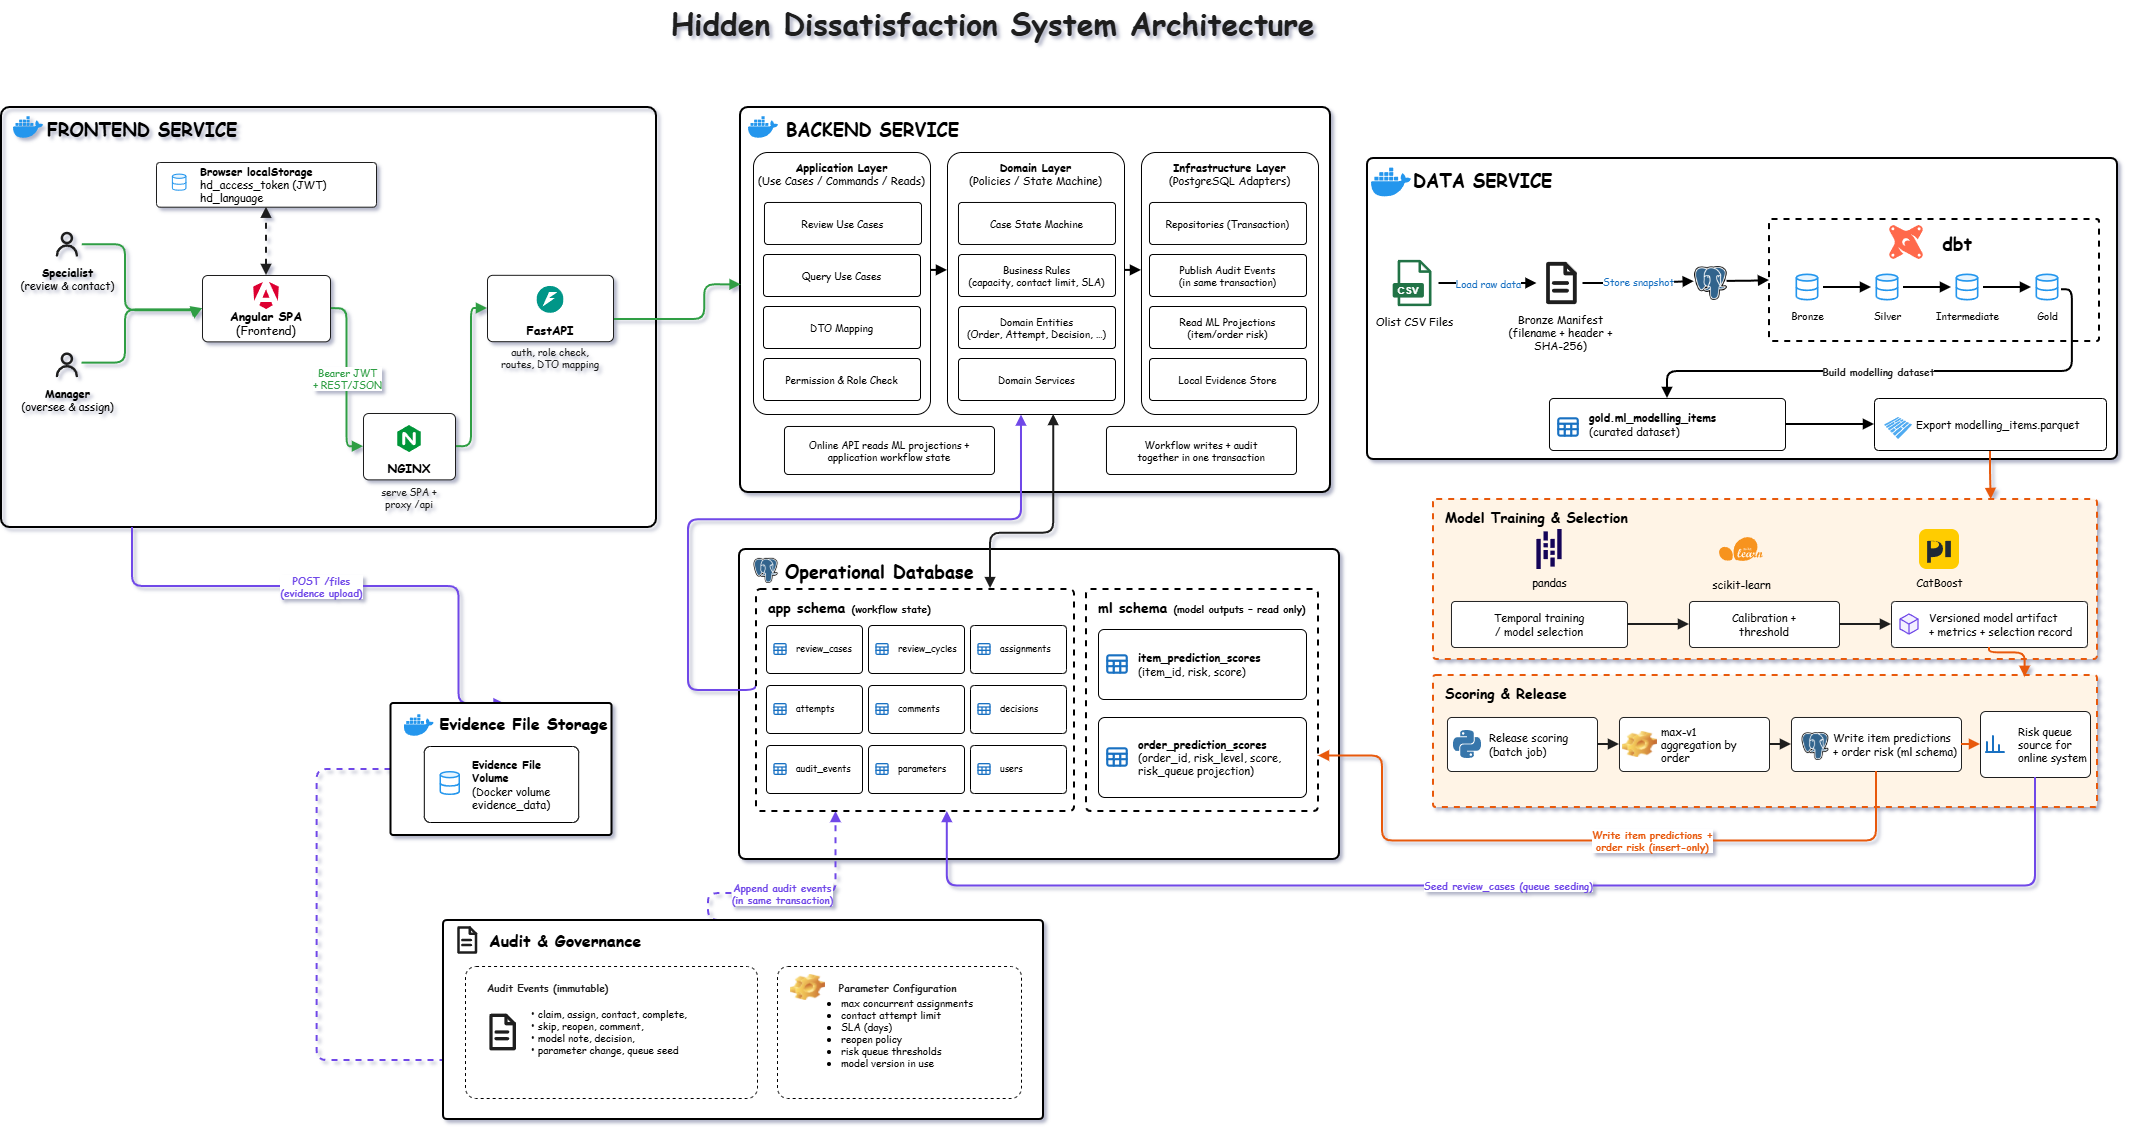
\includegraphics[width=\linewidth]{system-architecture}
  \caption{Kiến trúc tổng thể hệ thống}\label{fig:arch}
\end{figure}

\subsection{Đặc tả hệ thống}

Hệ thống được tổ chức theo kiến trúc phân lớp. Mỗi lớp chỉ đảm nhận một loại trách nhiệm, nhờ đó có thể thay mô hình học máy mà không phải sửa các lớp khác:
\begin{itemize}
  \item \textbf{Miền nghiệp vụ} (domain): điều kiện vào quần thể, ý nghĩa nhãn, các bất biến về thời gian. Lớp này không phụ thuộc thư viện dữ liệu hay mô hình.
  \item \textbf{Ứng dụng} (application): điều phối các ca sử dụng như nạp dữ liệu, huấn luyện, chấm điểm.
  \item \textbf{Hạ tầng} (infrastructure): đọc ghi PostgreSQL, tính đặc trưng, huấn luyện và lưu mô hình.
  \item \textbf{Giao diện} (interfaces): giao diện dòng lệnh (CLI) cho các tác vụ theo lô, và API cho ứng dụng web.
\end{itemize}

\textbf{Cơ chế chấm điểm theo lô.} Mô hình không được gọi theo thời gian thực. Một tác vụ theo lô chấm điểm toàn bộ item, tổng hợp điểm đơn bằng \texttt{max-v1}, gán mức \textsc{Cao}/\textsc{Trung bình}/\textsc{Thấp} theo ngưỡng đã chọn rồi ghi vào bảng dự đoán. Mỗi bản ghi lưu mã đơn, điểm rủi ro, mức ưu tiên và phiên bản mô hình, nên có thể truy vết kết quả về đúng lần huấn luyện. Cách làm này giữ ứng dụng web đơn giản và đảm bảo mọi người dùng nhìn thấy cùng một kết quả.

\textbf{Ứng dụng vận hành.} Backend viết bằng FastAPI, frontend bằng Angular, toàn bộ dịch vụ (PostgreSQL, API, frontend, tác vụ kho dữ liệu) được đóng gói bằng Docker Compose. Ứng dụng phục vụ hai vai trò: \emph{chuyên viên} (Specialist) nhận và xử lý đơn mức thấp và trung bình, \emph{quản lý} (Manager) giao đơn mức cao, điều chỉnh tham số vận hành và ra quyết định. Các chức năng chính gồm:
\begin{itemize}
  \item \textbf{Hàng đợi rủi ro}: danh sách đơn sắp xếp theo điểm rủi ro giảm dần, sau đó theo hạn SLA và thời gian chờ; có thể lọc theo mức rủi ro, trạng thái, người bán, danh mục.
  \item \textbf{Chi tiết đơn}: điểm của từng sản phẩm trong đơn, ghi nhận các lần liên lạc với khách và kết quả xử lý.
  \item \textbf{Dashboard và lịch sử kiểm toán}: tổng hợp tình trạng xử lý; mọi thao tác ghi đều sinh một sự kiện kiểm toán chỉ được thêm, không được sửa hay xóa.
\end{itemize}

Ba nguyên tắc được áp dụng xuyên suốt. Thứ nhất, backend kiểm tra mọi luật nghiệp vụ (quyền theo vai, giới hạn số đơn mỗi người, số lần liên lạc tối đa), kể cả khi frontend đã ẩn nút tương ứng. Thứ hai, không có API nào sửa được điểm rủi ro hay mức rủi ro do mô hình tạo ra. Thứ ba, các tham số vận hành như giới hạn số đơn và thời hạn SLA được lưu trong cơ sở dữ liệu và do quản lý điều chỉnh, không ghi cứng trong mã nguồn.

% =====================================================================
\section{Dữ liệu và công cụ}\label{sec:data}

\subsection{Nguồn dữ liệu}

Nghiên cứu sử dụng bộ dữ liệu công khai \emph{Brazilian E-Commerce Public Dataset by Olist}~\cite{olist2018}, gồm khoảng 99\,000 đơn hàng phát sinh trên các sàn thương mại điện tử tại Brazil từ năm 2016 đến 2018. Dữ liệu gồm chín bảng liên kết với nhau qua các khóa \texttt{order\_id}, \texttt{customer\_id}, \texttt{product\_id} và \texttt{seller\_id} (Bảng~\ref{tab:olist}). Bảng đơn hàng là trung tâm, ghi các mốc thời gian của vòng đời đơn: mua, duyệt, bàn giao cho đơn vị vận chuyển, giao cho khách và ngày giao dự kiến. Các mốc này là cơ sở để xác định thời điểm dự đoán và lọc đơn giao đúng hạn.

\begin{table}[htbp]\centering\small
\caption{Các bảng trong bộ dữ liệu Olist}\label{tab:olist}
\begin{tabular}{llr}
\toprule
Bảng & Độ chi tiết (một dòng là) & Số dòng \\
\midrule
\texttt{orders}         & một đơn hàng                          &    99\,441 \\
\texttt{order\_items}   & một sản phẩm trong đơn                &   112\,650 \\
\texttt{order\_payments}& một lần thanh toán của đơn            &   103\,886 \\
\texttt{order\_reviews} & một đánh giá                          &    99\,224 \\
\texttt{customers}      & một khách hàng theo đơn               &    99\,441 \\
\texttt{sellers}        & một người bán                         &     3\,095 \\
\texttt{products}       & một sản phẩm                          &    32\,951 \\
\texttt{geolocation}    & một tọa độ theo mã bưu chính          & 1\,000\,163 \\
\texttt{category\_translation} & một danh mục (tiếng Bồ Đào Nha -- Anh) & 71 \\
\bottomrule
\end{tabular}
\end{table}

Có hai đặc điểm cần lưu ý. Bảng đánh giá có 99\,224 dòng nhưng một số đơn có nhiều đánh giá và một số đơn không có đánh giá nào. Bảng thanh toán có thể có nhiều dòng cho một đơn khi khách trả bằng nhiều phương thức. Cả hai bảng vì vậy phải được gộp về mức đơn trước khi nối với bảng sản phẩm trong đơn.

\subsection{Xây dựng tập dữ liệu mô hình hóa}

Bảng mô hình hóa có độ chi tiết là item. Bảng thanh toán và bảng đánh giá vốn ở mức đơn, nên được gộp về một dòng mỗi đơn trước khi nối, tránh nhân bản item. Khi một đơn có nhiều đánh giá, nhóm chọn một đánh giá đại diện theo thứ tự ưu tiên: đánh giá đã được người bán trả lời, sau đó đánh giá có thời điểm trả lời hoặc tạo mới nhất, cuối cùng là mã đánh giá. Quy tắc này mang tính tất định, nên chạy lại luôn cho cùng kết quả.

Quần thể nghiên cứu gồm các đơn thỏa mãn đồng thời: (i) trạng thái \texttt{delivered}; (ii) ngày giao thực tế không muộn hơn ngày giao dự kiến; (iii) có đánh giá được tạo \emph{sau} thời điểm giao. Điều kiện (iii) loại các đánh giá tạo trước hoặc đúng lúc giao, vì khi đó không thể dự đoán trước khi nhãn xuất hiện. Bảng~\ref{tab:funnel} cho thấy số đơn và item còn lại sau mỗi bước lọc.

\begin{table}[htbp]\centering\small
\caption{Quá trình lọc quần thể nghiên cứu}\label{tab:funnel}
\begin{tabular}{lrr}
\toprule
Bước lọc & Đơn & Item \\
\midrule
Toàn bộ đơn hàng                          & 99\,441 & 112\,650 \\
Trạng thái \texttt{delivered}             & 96\,478 & 110\,197 \\
Giao đúng hoặc sớm hạn                    & 88\,644 & 101\,475 \\
Có đánh giá hợp lệ tạo sau thời điểm giao & 85\,420 &  97\,878 \\
\bottomrule
\end{tabular}
\end{table}

Tỉ lệ đơn nhận đánh giá thấp trong quần thể là 9,21\% (7\,865/85\,420), cho thấy bài toán mất cân bằng lớp rõ rệt. Bảng~\ref{tab:funnel} được dựng lại từ các tệp CSV gốc để kiểm toán. Snapshot dữ liệu đóng băng dùng cho huấn luyện có 85\,425 đơn và 97\,884 item, lệch 5 đơn và 6 item so với bản dựng lại. Nhật ký dbt xác nhận snapshot được tạo thành công và qua các kiểm tra về độ chi tiết và tính duy nhất, nhưng không lưu số đếm theo từng bước lọc nên chưa giải thích được chênh lệch này. Các thí nghiệm sử dụng số liệu của snapshot đóng băng.

\subsection{Đặc trưng và kiểm soát rò rỉ dữ liệu}

Mọi đặc trưng phải biết được tại thời điểm $t_o$. Nhóm cho phép các nhóm thông tin sau: thông tin đơn và thanh toán; thuộc tính sản phẩm, danh mục và người bán; vị trí của khách và người bán; giá, phí vận chuyển và cấu trúc đơn; thời gian giao và khoảng dư so với ngày dự kiến; và các đặc trưng lịch sử tính hoàn toàn từ sự kiện xảy ra trước $t_o$. Các đầu vào sau bị cấm: điểm, nội dung, tiêu đề và thời điểm của đánh giá; mọi hành động xảy ra sau đánh giá; các thống kê tính trên toàn bộ dữ liệu; và các mã định danh. Pipeline từ chối tự động mọi cột thuộc nhóm bị cấm hoặc không có trong danh sách khai báo. Hình~\ref{fig:leakage-timeline} minh họa ranh giới này.

\begin{figure}[htbp]\centering
\begin{tikzpicture}[x=1cm,y=1cm,font=\small,
  ev/.style={circle,fill,inner sep=1.5pt},
  lab/.style={align=center,font=\footnotesize}]
  \fill[green!12] (0,0) rectangle (9,1.2);
  \fill[red!12]   (9,0) rectangle (13.5,1.2);
  \node[lab,green!45!black] at (4.5,1.45) {Được dùng làm đặc trưng};
  \node[lab,red!60!black]   at (11.25,1.45) {Bị cấm (rò rỉ)};
  \draw[-{Latex}] (0,0) -- (13.7,0) node[right]{$t$};
  \node[ev] at (3,0) {};   \node[lab,below] at (3,-0.1) {Mua hàng};
  \node[ev] at (5.5,0) {}; \node[lab,below] at (5.5,-0.1) {Seller\\gửi hàng};
  \draw[very thick] (9,-0.3) -- (9,1.2);
  \node[lab,below] at (9,-0.3) {\textbf{Giao hàng}\\$t_o$ (thời điểm dự đoán)};
  \node[ev] at (11.5,0) {}; \node[lab,below] at (11.5,-0.1) {Tạo đánh giá\\(nhãn $y$)};
  \draw[|-|,thick,blue!60!black] (0.2,0.6) -- (9,0.6) node[midway,above,lab]{Lịch sử của seller/danh mục từ các đơn trước $t_o$};
\end{tikzpicture}
\caption{Ranh giới thời gian của đặc trưng. Đặc trưng lịch sử chỉ dùng sự kiện xảy ra trước $t_o$ (cận trên mở); thông tin đánh giá và mọi sự kiện sau $t_o$ bị loại.}
\label{fig:leakage-timeline}
\end{figure}

Đặc trưng lịch sử của người bán và danh mục (số đánh giá trước đó, điểm đánh giá trung bình, thời gian xử lý và giao hàng trung bình) chỉ được tính từ các đơn có cả thời điểm giao lẫn thời điểm đánh giá diễn ra \emph{trước} $t_o$ của đơn đang xét. Khi có ít hơn năm quan sát trước đó, giá trị trung bình được để trống và một cờ ``hỗ trợ thấp'' được bật, giúp mô hình phân biệt giữa ``không có lịch sử'' và ``lịch sử tốt''.

Tập đặc trưng cuối cùng (phiên bản \texttt{p5-item-v11-interactions}) gồm 61 đặc trưng chia thành bảy nhóm (Bảng~\ref{tab:features}). Việc đưa các đặc trưng về giao hàng và cấu trúc đơn được gợi ý từ các nghiên cứu cho thấy hiệu quả giao hàng ảnh hưởng đến điểm đánh giá~\cite{ravula2023,deshpande2023}, và giao hàng tách thành nhiều kiện có thể làm giảm sự hài lòng~\cite{brylla2022}. Olist không ghi thời điểm giao riêng cho từng item, nên số người bán và số sản phẩm trong đơn chỉ là đại diện gián tiếp cho việc tách đơn, không phải quan sát trực tiếp.

\begin{table}[htbp]\centering\small
\caption{Các nhóm đặc trưng trong tập cuối cùng}\label{tab:features}
\begin{tabular}{p{4.2cm}p{9cm}}
\toprule
Nhóm & Nội dung chính \\
\midrule
Cơ sở (24) & Giá, phí vận chuyển, thanh toán, thời gian giao, khoảng dư so với ngày dự kiến, kích thước sản phẩm, lịch sử đánh giá của seller và danh mục kèm cờ hỗ trợ thấp, danh mục, bang của khách \\
Tốc độ và độ biến động của seller (7) & Thời gian trung bình từ duyệt đơn đến bàn giao vận chuyển và đến khi giao, độ lệch chuẩn, hệ số biến thiên, tỉ lệ phí vận chuyển \\
Số lượng trong đơn (7) & Số seller, danh mục, sản phẩm; cờ nhiều item, nhiều seller, nhiều danh mục \\
Tỉ lệ trong đơn (4) & Tổng phí vận chuyển, tỉ trọng phí vận chuyển, tỉ trọng giá trị lớn nhất và nhỏ nhất của item \\
Mức độ tập trung (2) & Chỉ số Herfindahl--Hirschman theo danh mục và theo seller \\
Hình thái sản phẩm (13) & Thể tích, mật độ, tỉ lệ kích thước, phí vận chuyển trên giá và trên khối lượng, các cờ thiếu hoặc bằng không \\
Độ đầy đủ nội dung (4) & Độ dài tên và mô tả, số trường mô tả bị thiếu \\
\bottomrule
\end{tabular}
\end{table}
% Danh sách đầy đủ 61 cột: đưa vào Phụ lục (SERVER_CONTEXT/chapter3_evidence.md §5).

\subsection{Công cụ}

Pipeline được viết bằng Python 3.11 với pandas 2.3.3, NumPy 2.4.6 và PyArrow 21.0.0 để xử lý dữ liệu; scikit-learn 1.9.1 và CatBoost 1.2.10 để huấn luyện mô hình; joblib 1.6.0 để lưu mô hình. Kho dữ liệu dùng PostgreSQL với các phép biến đổi viết bằng dbt 1.8.10. Toàn bộ ranh giới thời gian, danh sách biến thể và siêu tham số được khai báo trong một tệp cấu hình TOML có quản lý phiên bản, thay vì nằm rải rác trong notebook. Mọi lần chạy dùng seed cố định 42 và giới hạn số luồng để kết quả lặp lại được. Mỗi lần chạy xuất một báo cáo JSON ghi lại cấu hình, số liệu theo phân vùng, chỉ số và mã commit Git. GPU chỉ được dùng cho các biến thể CatBoost; mô hình được giữ lại chạy trên CPU.

Kho dữ liệu được tổ chức theo kiến trúc medallion. Tầng \emph{bronze} lưu dữ liệu nguyên dạng từ các tệp CSV kèm manifest chống nạp trùng. Tầng \emph{silver} chuẩn hóa kiểu dữ liệu và gộp tọa độ theo mã bưu chính. Tầng \emph{intermediate} chứa các mô hình dbt tính quần thể nghiên cứu, đánh giá đại diện, đặc trưng lịch sử và các nhóm đặc trưng trong Bảng~\ref{tab:features}. Tầng \emph{gold} gồm các bảng sự kiện và chiều phục vụ dashboard (đơn hàng, sản phẩm trong đơn, thanh toán, đánh giá, người bán, sản phẩm, khách hàng) và bảng \texttt{ml\_modelling\_items} phục vụ huấn luyện. Sau mỗi lần build, dbt chạy các kiểm tra tự động về tính duy nhất của khóa và độ chi tiết của bảng; các đặc trưng lịch sử có kiểm thử đơn vị riêng để đảm bảo không dùng sự kiện từ tương lai.

% =====================================================================
\section{Mô hình và thuật toán}\label{sec:models}

\subsection{Mô hình cơ sở và ứng viên}

Nhóm so sánh các mô hình theo thứ tự độ phức tạp tăng dần:
\begin{itemize}
  \item \textbf{Mô hình theo tỉ lệ nền} (prevalence): dự đoán mọi item bằng tỉ lệ dương của tập huấn luyện. Mô hình này là mức sàn mà mọi ứng viên phải vượt qua.
  \item \textbf{Hồi quy logistic} với hai mức điều chuẩn $C \in \{0{,}1;\,1\}$.
  \item \textbf{Rừng ngẫu nhiên} (Random Forest) với hai cấu hình: (độ sâu 8, tối thiểu 5 mẫu mỗi lá) và (độ sâu 12, tối thiểu 10 mẫu mỗi lá).
  \item \textbf{HistGradientBoosting} với hai cấu hình: (L2 $=1$, 31 lá) và (L2 $=5$, 15 lá).
  \item \textbf{CatBoost} chạy trên GPU, dùng cơ chế xử lý biến phân loại có sẵn, với độ sâu 6, 8 và 10.
\end{itemize}

Bên cạnh mô hình, nhóm thử bốn chế độ huấn luyện: \emph{item-unweighted} (mỗi item có trọng số như nhau), \emph{order-weight} (trọng số mỗi item bằng nghịch đảo số item trong đơn, để mỗi đơn đóng góp như nhau), \emph{order-reference} và \emph{order-aggregate} (gộp item thành một dòng mỗi đơn trước khi huấn luyện). Chế độ order-aggregate được thêm vào vì nhãn và chỉ số chính đều ở mức đơn.

\subsection{Tiền xử lý}

Mỗi họ mô hình có một nhánh tiền xử lý riêng. Với hồi quy logistic và rừng ngẫu nhiên, biến số được điền giá trị thiếu bằng trung vị (hồi quy logistic có thêm chuẩn hóa), biến phân loại được điền bằng giá trị phổ biến nhất rồi mã hóa one-hot, bỏ qua các giá trị chưa gặp. Với HistGradientBoosting, biến phân loại được mã hóa thứ tự để giữ ma trận dày. CatBoost nhận trực tiếp biến phân loại. Mọi bước tiền xử lý được đặt trong cùng một pipeline với mô hình và chỉ được fit trên dữ liệu huấn luyện của từng fold, tránh để thống kê của tập kiểm định lọt vào quá trình huấn luyện.

\subsection{Xử lý mất cân bằng lớp}

Với tỉ lệ dương khoảng 9--14\%, nhóm xử lý mất cân bằng bằng trọng số lớp (ví dụ \texttt{class\_weight=balanced\_subsample} cho rừng ngẫu nhiên) kết hợp với chọn ngưỡng riêng, thay vì lấy mẫu lại dữ liệu. Lựa chọn này dựa trên hai bằng chứng. Thứ nhất, với các bộ phân loại mạnh như mô hình boosting, cân bằng dữ liệu bằng SMOTE hầu như không cải thiện so với việc tối ưu ngưỡng~\cite{elor2022smote}. Thứ hai, các phương pháp hiệu chỉnh mất cân bằng làm xác suất dự đoán bị lệch lên một cách có hệ thống, làm hỏng độ tin cậy của xác suất~\cite{vandengoorbergh2022}. Vì bài toán cần xác suất đáng tin để xếp hàng ưu tiên, SMOTE chỉ được xem là thí nghiệm phụ và chưa được đưa vào pipeline chính.

\subsection{Chia dữ liệu theo thời gian và lựa chọn mô hình}

Dữ liệu được sắp theo thời điểm dự đoán $t_o$ và chia thành sáu phân vùng liên tiếp (Bảng~\ref{tab:split}). Mỗi phân vùng là khoảng nửa mở $[\text{đầu}, \text{cuối})$ và mọi item của một đơn luôn nằm cùng phân vùng. Mỗi phân vùng chỉ phục vụ đúng một mục đích, nên không có quyết định nào được đưa ra trên dữ liệu đã dùng cho quyết định trước đó. Cách chia này khác với việc chia ngẫu nhiên 80:20 thường gặp trong các nghiên cứu trước trên Olist~\cite{orman2026}: chia ngẫu nhiên cho phép mô hình ``nhìn thấy tương lai'', nên thường cho kết quả lạc quan hơn thực tế triển khai.

\begin{table}[htbp]\centering\small
\caption{Phân vùng dữ liệu theo thời gian dự đoán}\label{tab:split}
\begin{tabular}{lllrrr}
\toprule
Phân vùng & Từ & Đến (không gồm) & Đơn & Item & Tỉ lệ dương \\
\midrule
Huấn luyện            & 2016-10-11 & 2017-10-01 & 23\,545 & 26\,708 & 10,13\% \\
Lựa chọn mô hình      & 2017-10-01 & 2017-12-01 &  8\,586 &  9\,957 & 11,92\% \\
Fit hiệu chỉnh        & 2017-12-01 & 2018-02-01 & 11\,759 & 13\,444 & 12,74\% \\
So sánh hiệu chỉnh    & 2018-02-01 & 2018-04-01 & 10\,623 & 12\,265 & 13,80\% \\
Chọn ngưỡng           & 2018-04-01 & 2018-06-01 & 12\,351 & 14\,319 & 11,61\% \\
Test niêm phong       & 2018-06-01 & 2018-09-01 & 18\,561 & 21\,191 & ẩn \\
\bottomrule
\end{tabular}
\end{table}

Trong giai đoạn huấn luyện, các biến thể được so sánh bằng kiểm định rolling-origin với cửa sổ mở rộng gồm ba fold (Hình~\ref{fig:temporal-folds}). Ở mỗi fold, mô hình học trên toàn bộ dữ liệu trước mốc cắt và được đánh giá trên đoạn ngay sau đó, mô phỏng đúng cách mô hình được dùng trong thực tế. Biến thể được chọn theo thứ tự ưu tiên: PR-AUC mức đơn (theo \texttt{max-v1}) trung bình qua các fold cao nhất; nếu ngang nhau thì chọn biến thể có Brier score thấp hơn; nếu vẫn ngang nhau thì chọn mô hình đơn giản hơn. Hiệu chỉnh xác suất và chọn ngưỡng không tham gia vào bước này.

\begin{figure}[htbp]\centering
\begin{tikzpicture}[x=0.62cm,y=1cm,font=\footnotesize]
  % trục: tháng 0 = 2016-10; 23 = 2018-09
  \def\seg#1#2#3#4{\fill[#3] (#1,0) rectangle (#2,0.6); \node[font=\scriptsize] at ({(#1+#2)/2},0.3) {#4};}
  \seg{0}{12}{blue!30}{Huấn luyện}
  \seg{12}{14}{orange!55}{A}
  \seg{14}{16}{teal!40}{B}
  \seg{16}{18}{teal!25}{C}
  \seg{18}{20}{violet!30}{D}
  \seg{20}{23}{red!50}{Test}
  % 3 fold rolling-origin trong train; mốc thật, đơn vị tháng từ 2016-10-01:
  % 2017-06-01=8.0, 2017-07-18=9.57, 2017-08-24=10.77, 2017-10-01=12.0
  \foreach \k/\s/\e in {1/8.0/9.57,2/9.57/10.77,3/10.77/12.0} {
    \fill[blue!30] (0,-0.4*\k) rectangle (\s,-0.4*\k+0.28);
    \fill[orange!55] (\s,-0.4*\k) rectangle (\e,-0.4*\k+0.28);
    \node[left] at (0,-0.4*\k+0.14) {Fold \k};
  }
  \draw[densely dotted] (8,-1.3) -- (8,-1.55) node[below,font=\scriptsize]{2017-06};
  \draw[-{Latex}] (0,-1.55) -- (23.6,-1.55);
  \foreach \m/\l in {0/2016-10,12/2017-10,14/2017-12,16/2018-02,18/2018-04,20/2018-06,23/2018-09}
    \draw (\m,-1.5) -- (\m,-1.6) node[below,rotate=40,anchor=north east,font=\scriptsize]{\l};
  \node[align=left,anchor=north west,font=\scriptsize] at (0,-2.7)
    {A: lựa chọn mô hình \quad B: fit hiệu chỉnh \quad C: so sánh hiệu chỉnh \quad D: chọn ngưỡng \quad Test: test niêm phong};
\end{tikzpicture}
\caption{Thiết kế chia dữ liệu theo thời gian. Ba fold rolling-origin với cửa sổ mở rộng nằm trong giai đoạn huấn luyện; đoạn kiểm định của các fold lần lượt bắt đầu ngày 2017-06-01, 2017-07-18 và 2017-08-24. Mọi sản phẩm của một đơn nằm cùng một phân vùng.}
\label{fig:temporal-folds}
\end{figure}

\subsection{Hiệu chỉnh xác suất và ngưỡng ưu tiên}

Trọng số lớp giúp mô hình chú ý đến lớp thiểu số nhưng làm xác suất đầu ra bị đẩy lên cao. Vì hàng đợi ưu tiên cần xác suất phản ánh đúng tỉ lệ thực tế, nhóm hiệu chỉnh xác suất sau khi đã chọn mô hình. Mô hình gốc được huấn luyện lại trên phân vùng huấn luyện và lựa chọn. Hai phương pháp hiệu chỉnh, sigmoid (Platt scaling) và isotonic, được fit trên phân vùng \emph{fit hiệu chỉnh}, rồi so sánh bằng Brier score trên phân vùng \emph{so sánh hiệu chỉnh} độc lập. Nếu không phương pháp nào cải thiện Brier score so với mô hình gốc, mô hình gốc được giữ nguyên. Tách riêng hai phân vùng giúp kết quả so sánh không bị lạc quan do đánh giá trên chính dữ liệu đã dùng để fit.

Ngưỡng ưu tiên được chọn trên phân vùng \emph{chọn ngưỡng}: các đơn thuộc 5\% điểm rủi ro cao nhất được gán mức \textsc{Cao}, các đơn còn lại trong 20\% cao nhất được gán mức \textsc{Trung bình}. Cách chọn theo tỉ lệ phần trăm gắn trực tiếp với năng lực xử lý của bộ phận chăm sóc khách hàng thay vì một ngưỡng xác suất cố định.

% =====================================================================
\section{Phương pháp đánh giá}\label{sec:eval}

Do lớp dương chỉ chiếm khoảng một phần mười, độ chính xác (accuracy) không có ý nghĩa: một mô hình dự đoán mọi đơn đều tốt đã đạt khoảng 90\%. Nhóm dùng ba chỉ số, tính trên đoạn kiểm định của từng fold rồi lấy trung bình qua ba fold.

\textbf{PR-AUC} (diện tích dưới đường cong precision--recall) là chỉ số chính, đo ở mức item và mức đơn (sau khi tổng hợp bằng \texttt{max-v1}). PR-AUC của một mô hình xếp hạng ngẫu nhiên xấp xỉ tỉ lệ dương, nên tỉ lệ dương của từng fold là mốc so sánh tự nhiên.

\textbf{Brier score} đo độ tin cậy của xác suất ở mức đơn:
\begin{equation}\label{eq:brier}
  \mathrm{BS} = \frac{1}{N}\sum_{j=1}^{N}\left(\hat{p}_j - y_j\right)^2
\end{equation}
trong đó $\hat p_j$ là xác suất dự đoán và $y_j \in \{0,1\}$ là nhãn thực tế; giá trị càng thấp càng tốt. Brier score cũng là tiêu chí so sánh các phương pháp hiệu chỉnh xác suất ở mục~\ref{sec:models}.

\textbf{Recall@5\%} đo hiệu quả ưu tiên: tỉ lệ đơn nhận đánh giá thấp nằm trong 5\% đơn có điểm rủi ro cao nhất. Mức 5\% tương ứng với nhóm ưu tiên \textsc{Cao}. Nếu chọn ngẫu nhiên 5\% số đơn, recall kỳ vọng chỉ là 5\%, nên đây là mốc để đánh giá giá trị của mô hình đối với bộ phận vận hành.

Các kết quả trình bày ở Chương~4 là kết quả trên các fold phát triển. Phân vùng test niêm phong chưa được dùng để đánh giá, vì vậy các con số mang tính thăm dò và chưa phải ước lượng cuối cùng về hiệu năng khi triển khai.


% Chương 4 — Kết quả và phân tích. Số liệu kết quả để ở đây; phương pháp ở Chương 3.
% Nguồn số liệu mô hình (4.2–4.4): SERVER_CONTEXT/chapter3_evidence.md, chapter4_evidence.md, model_variant_fold_metrics.md,
% reports/P5-accuracy-coursework-summary.md, P5-accuracy-failure-analysis.md, P5-S2/S4/S6/S10-*.md.
% Mọi kết quả mô hình là development/exploratory; không có kết quả test niêm phong. Brier so sánh hiệu chỉnh
% tính ở mức item, không trọng số (src/hidden_dissatisfaction/modeling/training.py, _select_calibration).
\chapter{Kết quả và phân tích}\label{ch:results}

% =====================================================================
% Mục EDA. Nguồn số liệu: notebooks/olist_open_eda.ipynb (EDA mở), notebooks/01_eda_why_lateness_dominates.ipynb
% (5 lý do giao trễ chi phối), và script tính trên quần thể nghiên cứu dựng lại từ data/raw/olist theo đúng luật
% int_p4_cohort.sql + int_p4_review_canonical.sql (kết quả khớp tab:funnel: 85 420 đơn / 97 878 item).
% Hình sao chép từ notebooks/figures/ (nhãn tiếng Anh giữ nguyên).
\section{Kết quả phân tích khám phá dữ liệu}\label{sec:eda}

Trước khi huấn luyện mô hình, nhóm khảo sát dữ liệu để trả lời hai câu hỏi. Câu thứ nhất là dữ liệu có đủ tin cậy để dựng quần thể và đặc trưng như mô tả ở Chương~\ref{ch:method} hay không; câu thứ hai là trong nhóm đơn giao đúng hạn còn lại những tín hiệu nào gắn với đánh giá thấp. Số liệu trong mục này thuộc ba mẫu khác nhau, và mỗi con số đều được ghi rõ mẫu của nó như sau.
\begin{itemize}
  \item \emph{Toàn bộ dữ liệu} Olist: 99\,441 đơn.
  \item \emph{Mẫu đã giao có đánh giá}: 95\,824 đơn đã giao, có ngày giao và có đánh giá, dùng khi so sánh đơn trễ với đơn đúng hạn. Ở mẫu này, một đơn được xem là trễ khi \emph{ngày} giao muộn hơn ngày dự kiến.
  \item \emph{Quần thể nghiên cứu} theo Bảng~\ref{tab:funnel}: 85\,420 đơn với 97\,878 item, dựng lại từ tệp CSV gốc bằng đúng luật lọc và luật chọn đánh giá của kho dữ liệu. Quần thể này so sánh ngày giao với ngày dự kiến theo mốc thời gian đầy đủ, nên số đơn ``đúng hạn'' của nó chênh vài nghìn đơn so với cách đếm theo ngày. Snapshot dùng để huấn luyện lệch so với bản dựng lại 5 đơn và 6 item.
\end{itemize}
Mọi kết quả trong mục là mô tả và tương quan, không mang ý nghĩa nhân quả.

\subsection{Độ phủ thời gian và chất lượng dữ liệu}\label{subsec:eda-coverage}

Dữ liệu Olist trải từ tháng 9/2016 đến tháng 10/2018 nhưng chỉ 20 tháng có mật độ đủ để phân tích (Hình~\ref{fig:eda-coverage}, các tháng tô xám là giai đoạn quá thưa). Từ tháng 1/2017 đến tháng 8/2018 có 99\,092 trong tổng số 99\,441 đơn. Năm 2016 gần như trống (tháng 11/2016 không có đơn nào), còn 20 đơn của tháng 9--10/2018 chưa từng được giao. Lượng đơn tăng nhanh trong năm 2017 rồi đi ngang ở mức 6\,200--7\,300 đơn mỗi tháng suốt năm 2018; tám tháng đầu năm 2018 có 53\,991 đơn, gấp khoảng 2,35 lần cùng kỳ năm 2017 (22\,968 đơn). Ngày Black Friday 24/11/2017 ghi nhận 1\,176 đơn, trong khi trung vị một ngày năm 2018 chỉ là 227 đơn. Vì năm 2016 quá thưa, phân vùng huấn luyện ở Bảng~\ref{tab:split} tuy bắt đầu từ tháng 10/2016 nhưng phần lớn dữ liệu của nó thuộc năm 2017.

\begin{figure}[htbp]\centering
  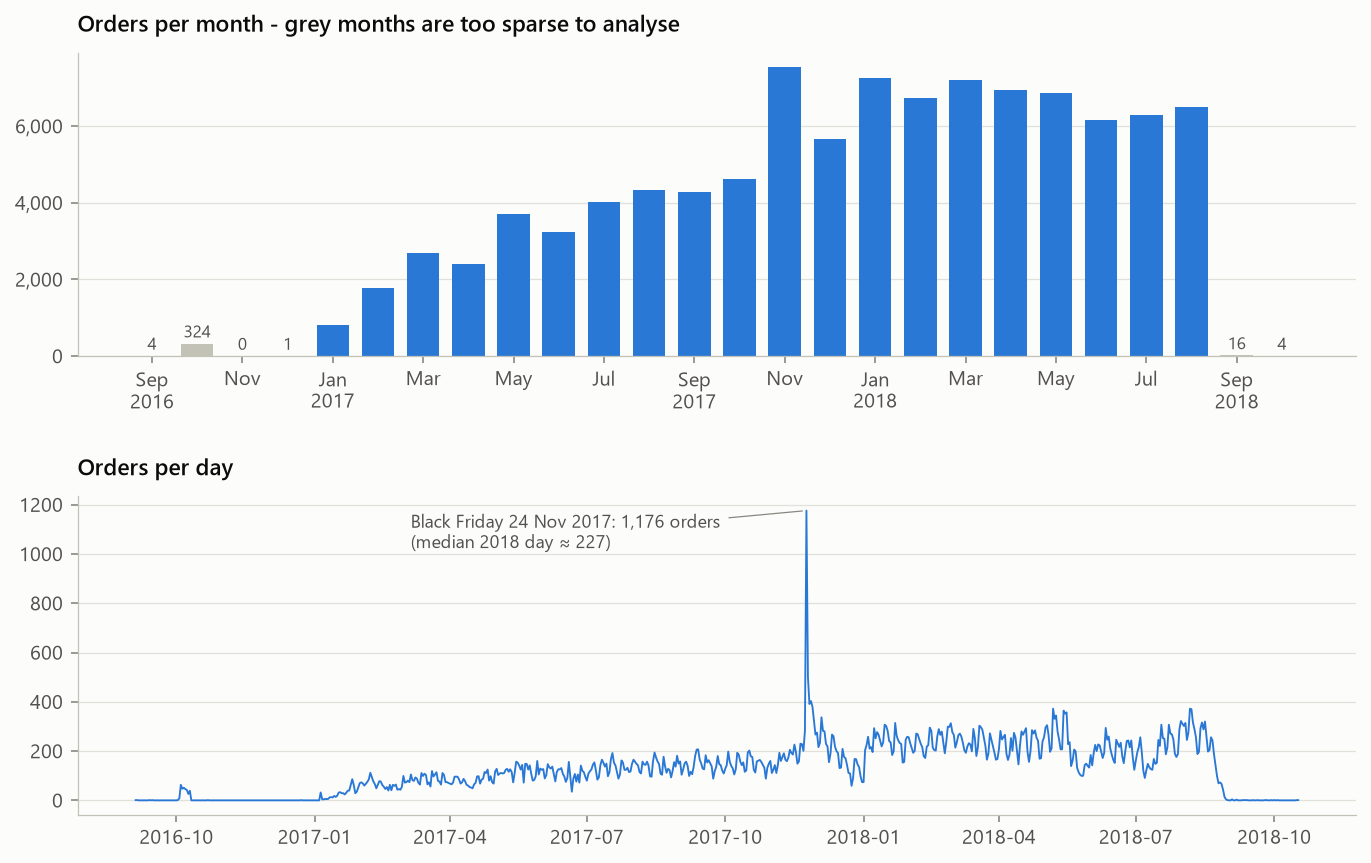
\includegraphics[width=\linewidth]{eda/01_coverage}
  \caption{Số đơn Olist theo tháng và theo ngày}
  \label{fig:eda-coverage}
\end{figure}

Hành vi vận hành cũng không đứng yên theo thời gian (Hình~\ref{fig:eda-operations}, tính theo tháng mua trên các đơn đã giao). Tỉ lệ giao trễ chỉ 3--5\% trong các tháng bình thường nhưng lên 12,4\% với đơn mua tháng 11/2017, 14,1\% với tháng 2/2018 và 19,0\% với tháng 3/2018 (vùng tô xám trong hình); điểm đánh giá trung bình giảm tương ứng xuống 3,91, 3,83 và 3,75, so với khoảng 4,2 ở các tháng khác. Thời gian giao dự kiến (trung vị) giảm từ 39 ngày vào tháng 1/2017 xuống khoảng 23 ngày từ giữa năm 2017 và còn 13,4 ngày vào tháng 8/2018. Cuộc đình công của tài xế xe tải cuối tháng 5/2018 kéo số đơn giao mỗi tuần từ khoảng 2\,000 xuống 634, và số người bán hoạt động mỗi tháng tăng từ 227 lên 1\,278. Những thay đổi chế độ vận hành này là bằng chứng trực tiếp cho lựa chọn chia dữ liệu theo thời gian thay vì chia ngẫu nhiên ở Chương~\ref{ch:method}, bởi một phép chia ngẫu nhiên sẽ trộn các giai đoạn có quy tắc hứa giao và tỉ lệ trễ rất khác nhau.

\begin{figure}[htbp]\centering
  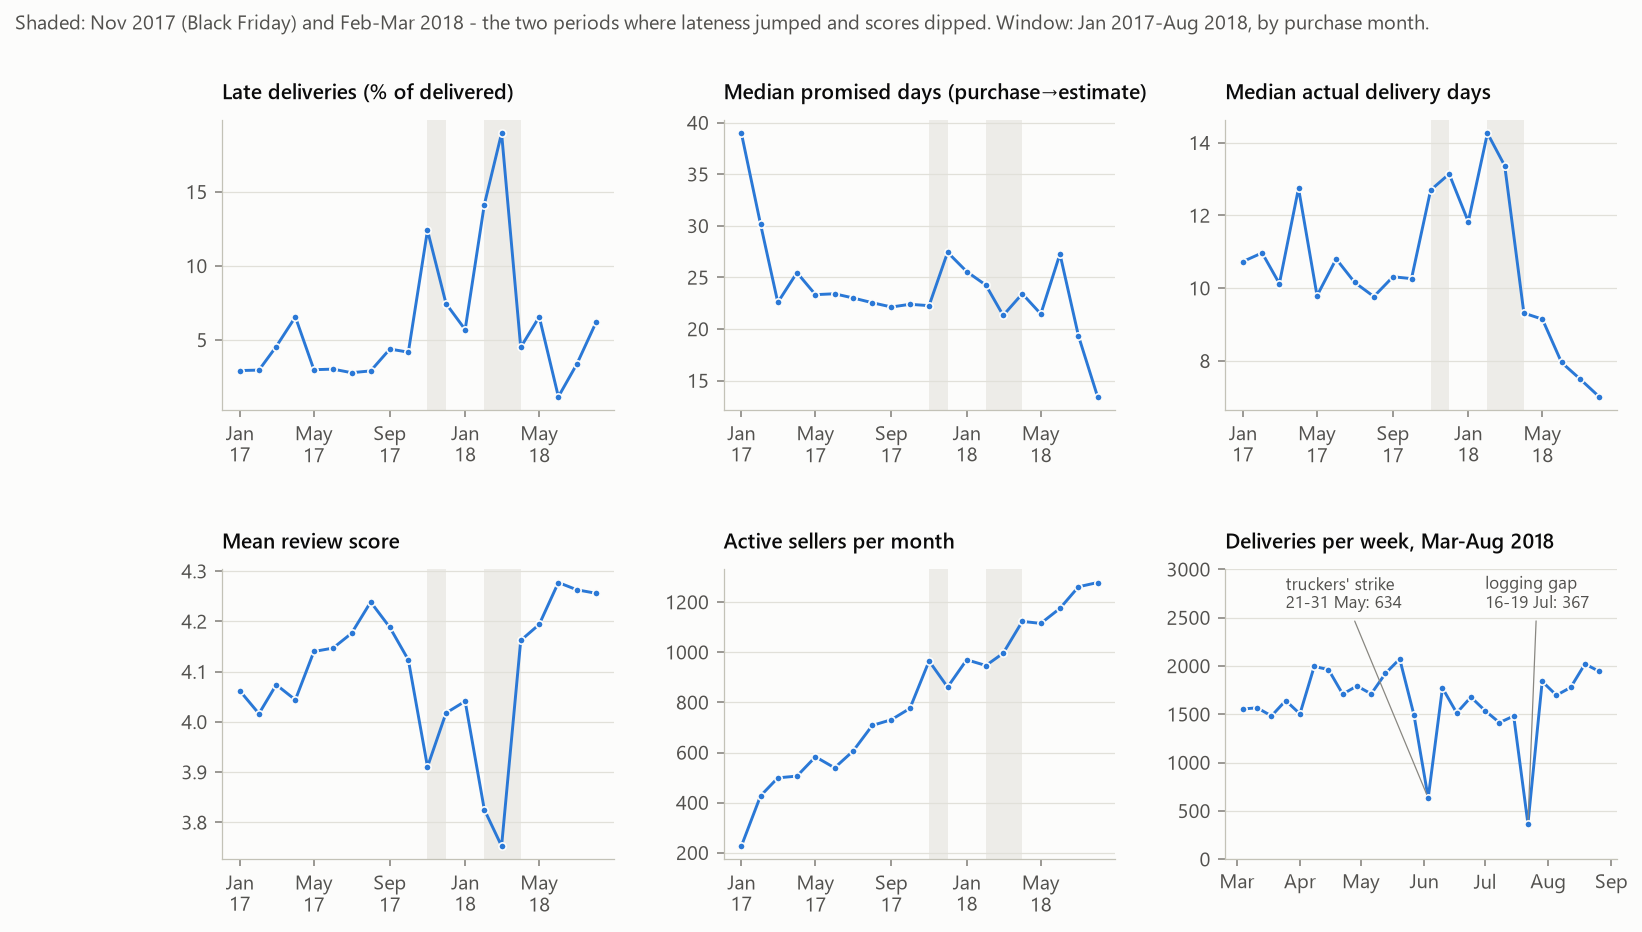
\includegraphics[width=\linewidth]{eda/03_operations_over_time}
  \caption{Diễn biến vận hành theo tháng mua}
  \label{fig:eda-operations}
\end{figure}

Kiểm tra chất lượng dữ liệu cho thấy bộ Olist nhìn chung sạch, nhưng có một số bẫy ảnh hưởng trực tiếp đến cách dựng quần thể. Nếu nối thẳng bảng đơn với bảng sản phẩm, thanh toán và đánh giá mà không gộp trước, kết quả có 117\,329 dòng cho 97\,916 đơn và doanh thu sản phẩm bị đếm thành 14,14 triệu real thay vì 13,59 triệu, đúng hiện tượng nhân bản dòng đã nêu ở Chương~\ref{ch:method}. Có 547 đơn mang 2--3 đánh giá, trong đó 202 đơn có các điểm số không thống nhất, nên cần một luật chọn đánh giá tất định như mô tả ở Chương~\ref{ch:method}; ngoài ra 789 mã đánh giá được dùng chung cho nhiều đơn, nên không thể khử trùng chỉ theo mã đánh giá.

Các mốc thời gian cũng có điểm bất thường. Có 1\,359 đơn có mốc bàn giao vận chuyển sớm hơn mốc duyệt thanh toán và 23 đơn có mốc giao cho khách sớm hơn mốc bàn giao; các khoảng thời gian âm này cần được đánh dấu thay vì tin tưởng. Hai khoảng 16--19/7/2018 và ngày 20/6/2017 gần như không có đơn được ghi nhận giao dù việc bàn giao vận chuyển vẫn diễn ra bình thường, nhiều khả năng là khoảng trống ghi log. Trong 96\,470 đơn đã giao có ngày giao, ngoài bình luận tùy chọn thì chỉ danh mục sản phẩm (1,41\%), đánh giá (0,67\%) và khoảng cách giữa người bán và khách hàng (0,49\%) có tỉ lệ thiếu đáng kể. Ở các bảng phụ, 610 sản phẩm không có danh mục, 26,2\% số dòng tọa độ là bản trùng hoàn toàn và 42 điểm tọa độ nằm ngoài lãnh thổ Brazil.

\subsection{Phân bố điểm đánh giá và mức mất cân bằng lớp}\label{subsec:eda-labels}

Điểm đánh giá có dạng chữ J quen thuộc (Hình~\ref{fig:eda-reviews}). Trên toàn bộ 99\,224 dòng đánh giá, 57,8\% là 5 sao, 19,3\% là 4 sao, 8,2\% là 3 sao, 3,2\% là 2 sao và 11,5\% là 1 sao. Khách không hài lòng viết bình luận nhiều hơn hẳn, với 77\% đánh giá 1 sao có bình luận so với 31\% ở mức 4 sao. Bình luận dồn ứ ở đúng 200 ký tự (659 bình luận), dấu hiệu văn bản đã bị cắt ngắn.

\begin{figure}[htbp]\centering
  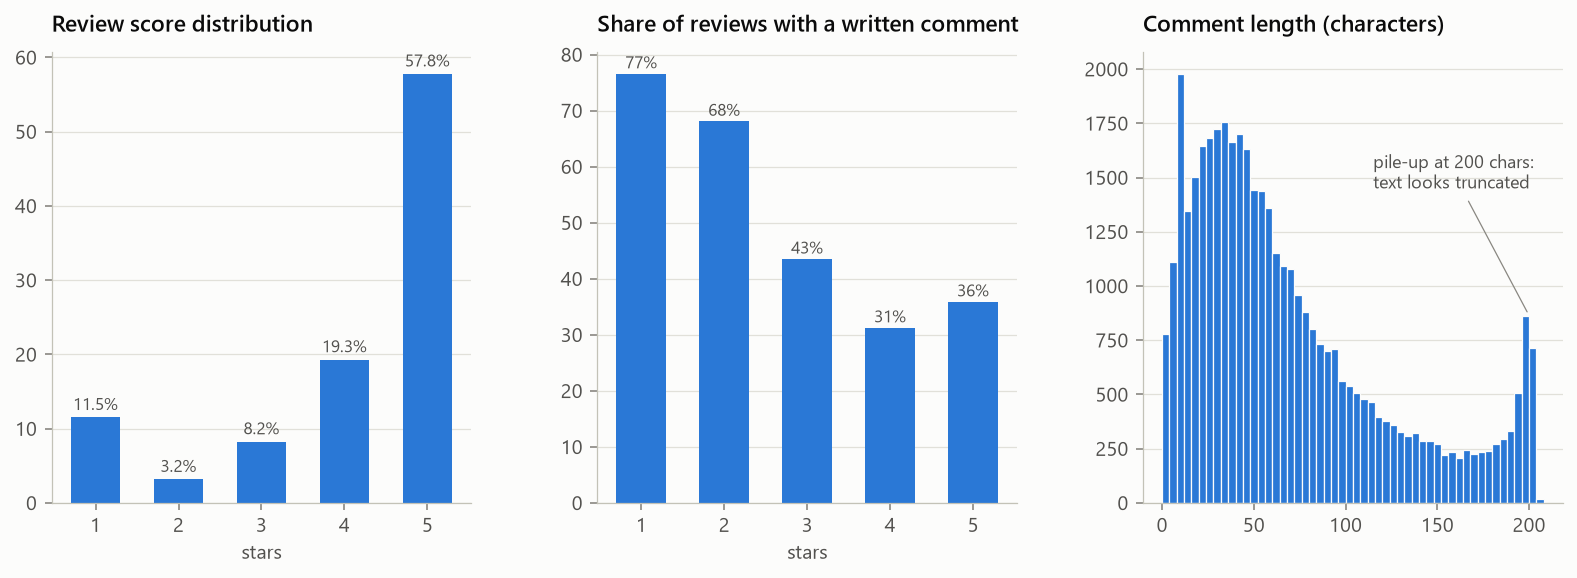
\includegraphics[width=\linewidth]{eda/13_reviews_overview}
  \caption{Phân bố điểm và bình luận đánh giá}
  \label{fig:eda-reviews}
\end{figure}

Trong quần thể nghiên cứu, phân bố dịch về phía hài lòng, với 62,45\% đơn nhận 5 sao, 20,35\% nhận 4 sao, 8,00\% nhận 3 sao, 2,63\% nhận 2 sao và 6,58\% nhận 1 sao. Tỉ lệ dương ở mức đơn vì vậy là 9,21\% (7\,865/85\,420), thấp hơn đáng kể so với 14,69\% khi tính trên mọi đơn có đánh giá. Ở mức item, tỉ lệ dương lên tới 11,41\% vì đơn nhiều sản phẩm có tỉ lệ bị đánh giá thấp cao hơn (mục~\ref{subsec:eda-ontime}) và đóng góp nhiều dòng hơn.

Khác biệt giữa hai mức này cần được ghi nhớ khi đọc Bảng~\ref{tab:split}. Tỉ lệ dương 10,13--13,80\% trong bảng đó được tính ở mức item, còn nếu dựng lại theo cùng mốc thời gian ở mức đơn thì tỉ lệ dương của năm phân vùng phát triển là 8,86--10,53\%. Theo tháng giao, tỉ lệ dương mức đơn của quần thể nghiên cứu dao động trong khoảng 7,8--10,9\%. Với khoảng một đơn dương trên mười một đơn, accuracy không phải thước đo phù hợp, như đã lập luận ở mục~\ref{sec:th-metrics}; tỉ lệ dương mức đơn này cũng là mốc ngẫu nhiên khi đọc PR-AUC ở mục~\ref{sec:results-analysis}.

\subsection{Vì sao giao trễ chi phối các mô hình dự báo hiện có}\label{subsec:eda-lateness}

Trên các đơn đã giao có đánh giá, giao trễ là tín hiệu mạnh nhất của đánh giá thấp. Theo định nghĩa trễ theo ngày, 6,7\% đơn bị giao trễ, và nhóm này có 62,4\% đơn bị đánh giá 1--2 sao, gấp 6,7 lần tỉ lệ 9,3\% của đơn đúng hạn. Hình~\ref{fig:eda-factors} đặt tám yếu tố trên cùng một thang đo, với đường xám là tỉ lệ chung 14,7\% trên mọi đơn có đánh giá; các ô về thời gian giao và khoảng cách chỉ tính trên đơn đã giao. Tỉ lệ đánh giá thấp chỉ 9\% với đơn giao sớm từ 7 ngày trở lên và 11\% với đơn giao sớm 0--6 ngày, nhưng lên 32\% khi trễ 1--3 ngày, 68\% khi trễ 4--7 ngày và 79\% khi trễ hơn 7 ngày. Quan hệ này có dạng bậc thang. Giao sớm hơn hứa hẹn hầu như không cải thiện thêm, nhưng chỉ cần vượt qua ngày hứa là tỉ lệ tăng vọt. Theo bảng chi tiết của notebook, tỉ lệ đánh giá thấp là 12,4\% với đơn giao đúng ngày dự kiến, 19,6\% khi trễ một ngày và 50,4\% khi trễ ba ngày. Dạng bất đối xứng này khớp với kết quả của \textcite{ravula2023} và với bằng chứng về tác động của chất lượng giao hàng lên điểm đánh giá~\parencite{deshpande2023}.

\begin{figure}[htbp]\centering
  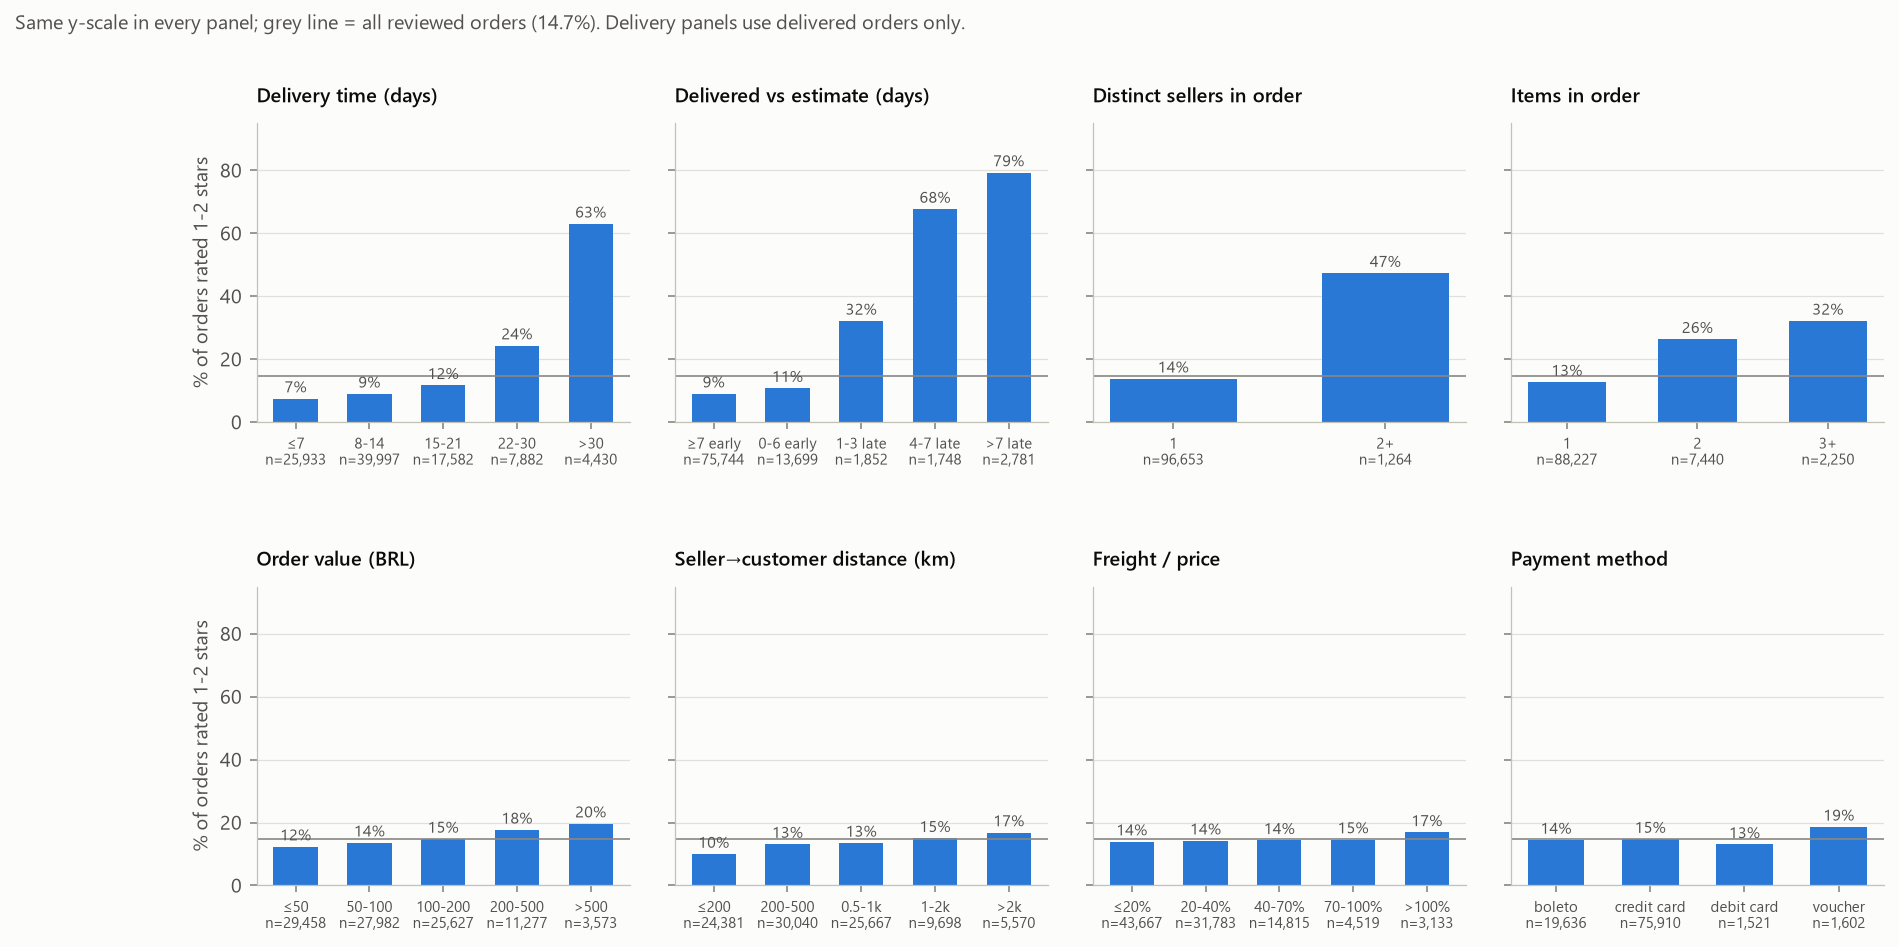
\includegraphics[width=\linewidth]{eda/14_score_factors}
  \caption{Tỉ lệ đánh giá 1--2 sao theo tám yếu tố}
  \label{fig:eda-factors}
\end{figure}

Phân tích trong notebook chỉ ra năm lý do khiến các mô hình hài lòng trên Olist hầu như đều ``phát hiện'' giao trễ là yếu tố quyết định (Bảng~\ref{tab:eda-reasons}). Lý do thứ hai đáng chú ý nhất vì nó nằm ở cơ chế sinh nhãn. Olist gửi khảo sát khi khách nhận hàng \emph{hoặc} khi đến ngày giao dự kiến~\parencite{olist2018}, nên với đơn trễ, khách thường được hỏi về một món hàng chưa nhận được. Trong mẫu đơn trễ, 70,1\% đánh giá được trả lời trước khi hàng đến và 80,8\% số đánh giá này là 1--2 sao; ngược lại, ở đơn đúng hạn chỉ 0,3\% khảo sát được gửi trước ngày giao. Với phần lớn đơn trễ, ``đánh giá'' thực chất là lời phàn nàn hàng chưa tới, và dự báo nó từ mốc thời gian gần như là dự báo lịch gửi khảo sát. Quần thể nghiên cứu loại bỏ vấn đề này từ gốc, vì chỉ giữ đơn giao đúng hạn và có đánh giá tạo sau thời điểm giao.

\begin{table}[htbp]\centering\small
\caption{Năm lý do giao trễ chi phối các mô hình dự báo hài lòng trên Olist (mẫu: 95\,824 đơn đã giao có đánh giá; trễ tính theo ngày)}\label{tab:eda-reasons}
\begin{tabular}{p{4.3cm}p{9.2cm}}
\toprule
Lý do & Bằng chứng \\
\midrule
Giao trễ là tín hiệu mạnh và có dạng bậc thang & 62,4\% đơn trễ bị đánh giá thấp so với 9,3\% đơn đúng hạn; trễ ba ngày đã có 50,4\% đơn bị đánh giá thấp (Hình~\ref{fig:eda-factors}) \\
Nhãn của đơn trễ phần lớn do lịch gửi khảo sát tạo ra & 70,1\% đánh giá của đơn trễ được viết trước khi hàng đến, 80,8\% trong số đó là 1--2 sao \\
Giao trễ quyết định các biến động theo thời gian & Tỉ lệ đánh giá thấp toàn bộ dao động 9,4--21,2\% theo tháng và tăng cùng tỉ lệ trễ (14,0\% tháng 2/2018, 18,7\% tháng 3/2018); tỉ lệ ở đơn đúng hạn chỉ dao động 7,4--10,7\% \\
Đặc trưng thời gian đứng đầu khi gộp mọi đơn & ROC-AUC đơn biến của bốn đặc trưng thời gian đứng đầu là 0,65--0,69 trên mọi đơn, nhưng các đặc trưng này chỉ đạt 0,51--0,57 trên đơn đúng hạn; ở nhóm này số item trong đơn (0,59), tỉ lệ đánh giá thấp trước đó của người bán (0,59) và phí vận chuyển (0,58) dẫn đầu \\
Accuracy che giấu vấn đề & Một mô hình boosting chẩn đoán (chia ngẫu nhiên 70/30, ngưỡng 0,5, như các nghiên cứu trước) đạt accuracy 89,8\%, chỉ hơn mức luôn dự đoán ``không tiêu cực'' (87,2\%) 2,6 điểm; 58,7\% danh sách 10\% rủi ro cao nhất là đơn trễ dù đơn trễ chỉ chiếm 6,7\%, và danh sách này bắt được 96,5\% đơn trễ bị đánh giá thấp nhưng chỉ 16,7\% đơn đúng hạn bị đánh giá thấp \\
\bottomrule
\end{tabular}
\end{table}

Hệ quả là các mô hình huấn luyện trên mọi đơn học chủ yếu cách nhận diện đơn trễ, trong khi phần lớn đánh giá thấp lại nằm ở nhóm còn lại. Trong 12\,272 đơn bị đánh giá 1--2 sao thuộc mẫu đã giao có đánh giá, 8\,289 đơn (67,5\%) đến từ đơn giao đúng hạn theo định nghĩa theo ngày; dùng định nghĩa theo mốc thời gian của quần thể nghiên cứu, con số là 8\,130 đơn (66,25\%). Đơn đúng hạn cũng là trạng thái phổ biến chứ không phải ngoại lệ (Hình~\ref{fig:eda-promise}). Trung vị thời gian giao thực tế là 10,2 ngày so với 23,2 ngày hứa giao, và 93,2\% đơn đến đúng hoặc sớm hạn với trung vị sớm 12 ngày. Theo tháng, tỉ lệ đánh giá thấp của đơn đúng hạn chỉ dao động trong khoảng 7,4--10,7\% (Bảng~\ref{tab:eda-reasons}), nên nhóm khách này không bao giờ hiện lên thành một đỉnh trên biểu đồ vận hành. Đó chính là lý do sự bất mãn của họ được gọi là ``ẩn''.

\begin{figure}[htbp]\centering
  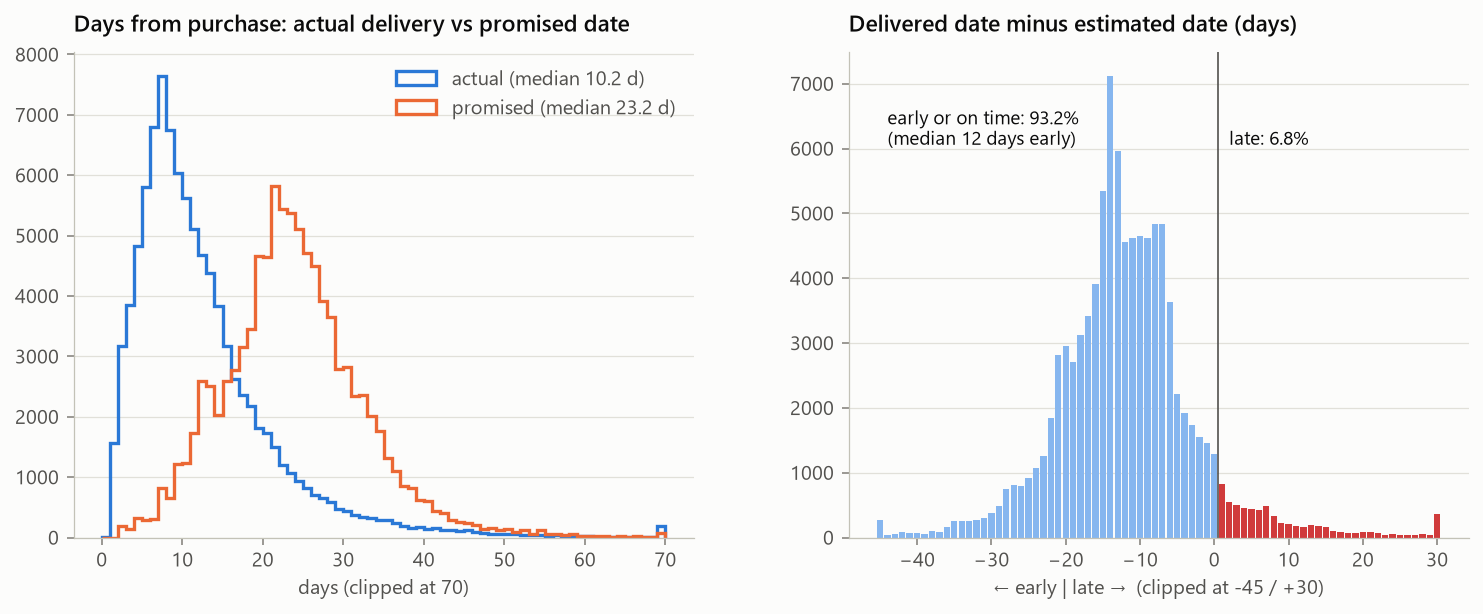
\includegraphics[width=\linewidth]{eda/09_promise_vs_reality}
  \caption{Thời gian giao thực tế so với thời gian hứa giao}
  \label{fig:eda-promise}
\end{figure}

\subsection{Tín hiệu trong nhóm đơn giao đúng hạn}\label{subsec:eda-ontime}

Khi đã loại giao trễ, các tín hiệu còn lại yếu hơn nhưng không biến mất. Bảng~\ref{tab:eda-segments} tóm tắt tỉ lệ đánh giá thấp mức đơn trong quần thể nghiên cứu theo các yếu tố đều biết được tại thời điểm giao. Cấu trúc đơn tạo khác biệt lớn nhất. Đơn có hai người bán bị đánh giá thấp 45,7\%, gấp hơn năm lần đơn một người bán (8,7\%), và tỉ lệ tăng đều từ 7,5\% ở đơn một item lên 31,9\% ở đơn từ bốn item. Nhóm đơn nhiều người bán rất nhỏ (1\,214 đơn), nhưng tỉ lệ 45,7--63,2\% của nó đã ngang với mức 62,4\% của đơn \emph{trễ} ở mục~\ref{subsec:eda-lateness}. Ở toàn bộ dữ liệu, đơn nhiều người bán còn có tỉ lệ trễ ghi nhận chỉ 1,0\% so với 6,9\% của đơn một người bán và điểm trung bình 2,86 so với 4,12, cho thấy mốc giao duy nhất của đơn nhiều khả năng chỉ phản ánh kiện hàng đến trước. Quan sát này khớp với bằng chứng rằng giao hàng tách kiện làm giảm sự hài lòng~\parencite{brylla2022}.

\begin{table}[htbp]\centering\small
\caption{Tỉ lệ đơn bị đánh giá 1--2 sao trong quần thể nghiên cứu theo một số yếu tố biết được tại thời điểm giao (85\,420 đơn dựng lại; tỉ lệ chung 9,21\%; mỗi yếu tố chỉ trình bày một số nhóm tiêu biểu)}\label{tab:eda-segments}
\begin{tabular}{llrr}
\toprule
Yếu tố & Nhóm & Số đơn & Tỉ lệ đánh giá thấp \\
\midrule
Số người bán trong đơn & 1 & 84\,206 & 8,7\% \\
 & 2 & 1\,157 & 45,7\% \\
 & 3 trở lên & 57 & 63,2\% \\
\addlinespace
Số item trong đơn & 1 & 76\,678 & 7,5\% \\
 & 2 & 6\,695 & 23,2\% \\
 & 3 & 1\,191 & 27,0\% \\
 & 4 trở lên & 856 & 31,9\% \\
\addlinespace
Số ngày từ mua đến giao & $\le$3 & 4\,622 & 6,6\% \\
 & 7--14 & 38\,328 & 8,7\% \\
 & 21--30 & 5\,164 & 14,6\% \\
 & $>$30 & 786 & 22,4\% \\
\addlinespace
Số ngày giao sớm so với dự kiến & 0--3 & 4\,505 & 11,3\% \\
 & 14--21 & 23\,515 & 8,3\% \\
 & $>$30 & 2\,256 & 11,0\% \\
\addlinespace
Bàn giao vận chuyển sau hạn & Không & 79\,118 & 8,9\% \\
 & Có & 6\,302 & 13,6\% \\
\addlinespace
Giá trị sản phẩm (real) & $\le$50 & 25\,911 & 7,8\% \\
 & $>$500 & 3\,020 & 12,9\% \\
\addlinespace
Phí vận chuyển / giá & $\le$20\% & 38\,050 & 8,8\% \\
 & $>$100\% & 2\,663 & 10,6\% \\
\addlinespace
Thanh toán đầu tiên & Thẻ tín dụng & 65\,863 & 9,2\% \\
 & Boleto & 16\,904 & 9,2\% \\
 & Voucher & 1\,342 & 10,5\% \\
\bottomrule
\end{tabular}
\end{table}

Đúng hạn không đồng nghĩa với nhanh. Đơn giao trong vòng ba ngày bị đánh giá thấp 6,6\%, còn đơn mất hơn 30 ngày dù vẫn kịp hạn có tỉ lệ 22,4\%. Khách đánh giá cả độ dài thời gian chờ chứ không chỉ việc lời hứa có được giữ hay không. Khoảng dư so với ngày dự kiến lại có dạng chữ U. Đơn kịp hạn sát nút (0--3 ngày) có tỉ lệ 11,3\%, đơn sớm 14--21 ngày có tỉ lệ thấp nhất 8,3\%, và đơn sớm hơn 30 ngày tăng trở lại 11,0\%, nhiều khả năng vì những đơn này đi kèm thời hạn hứa giao rất dài. Người bán bàn giao vận chuyển sau hạn gửi hàng nhưng hàng vẫn đến kịp có tỉ lệ 13,6\%, so với 8,9\% ở trường hợp còn lại. Lịch sử của người bán cũng mang tín hiệu. Trên mẫu đơn đúng hạn theo ngày của notebook (89\,443 đơn), người bán có hơn 30\% đánh giá thấp trong quá khứ tạo ra 18,4\% đánh giá thấp, so với 6,5\% ở người bán có tỉ lệ quá khứ từ 5\% trở xuống; tỉ lệ quá khứ này chỉ tính trên các đánh giá đã có trước thời điểm mua.

Danh mục sản phẩm tạo khác biệt vừa phải. Tính ở mức item trong quần thể nghiên cứu với các danh mục có từ 800 item, nội thất văn phòng có tỉ lệ dương cao nhất (22,4\% trên 1\,460 item), tiếp theo là đồ trang trí nội thất (14,9\%), chăn ga gối (14,8\%) và phụ kiện máy tính (14,0\%); thấp nhất là phụ kiện hành lý (6,5\%) và văn phòng phẩm (7,6\%). Các item thiếu danh mục có tỉ lệ 15,1\% (1\,344 item), vì vậy giữ ``thiếu danh mục'' thành một nhóm riêng có lợi hơn là điền giá trị. Các yếu tố tiền tệ dịch chuyển ít hơn. Tỉ lệ tăng từ 7,8\% ở đơn dưới 50 real lên 12,9\% ở đơn trên 500 real, còn tỉ trọng phí vận chuyển (8,8--10,6\%) và phương thức thanh toán (8,5--10,5\%) gần như phẳng. Theo bang của khách (các bang có từ 1\,000 đơn), tỉ lệ dao động từ 8,6\% ở São Paulo đến 10,9\% ở Rio de Janeiro và 11,1\% ở Bahia.

Ma trận tương quan Spearman trên 96\,470 đơn đã giao cho thấy vì sao các tín hiệu này khó nắm bắt bằng quan hệ tuyến tính. Không biến số mức đơn nào có hệ số tương quan Spearman với điểm đánh giá vượt quá 0,25 về độ lớn; mạnh nhất là số ngày giao ($-0{,}23$), thời gian vận chuyển ($-0{,}19$), chênh lệch so với ngày dự kiến ($-0{,}18$) và số item ($-0{,}11$). Các quan hệ ở Bảng~\ref{tab:eda-segments} có dạng ngưỡng hoặc chữ U, điều mà tương quan đơn điệu đánh giá thấp. Nhiều cặp biến giải thích lại đi cùng nhau, như số ngày giao và thời gian vận chuyển ($0{,}89$), giá trị đơn và tỉ trọng phí vận chuyển ($-0{,}78$), khoảng cách và số ngày hứa giao ($0{,}62$). Mô hình tuyến tính vì thế dễ gặp đa cộng tuyến, còn mô hình cây có thể tách các ngưỡng mà không cần chỉ định trước dạng quan hệ.

\subsection{Nội dung đánh giá của khách không hài lòng}\label{subsec:eda-text}

Văn bản đánh giá chỉ xuất hiện \emph{sau} khi khách đánh giá, nên nó không được dùng làm đặc trưng (Hình~\ref{fig:leakage-timeline}); nhóm chỉ dùng nó để hiểu nhãn. Theo luật từ khóa trên bình luận tiếng Bồ Đào Nha đã bỏ dấu (Hình~\ref{fig:eda-themes}), bình luận 1 sao chủ yếu nói hàng chưa tới (31\%), sau đó là hoàn tiền, trả hàng hoặc hủy đơn (10\%), thiếu một phần đơn (9\%), giao chậm (7\%), lỗi hoặc hư hỏng (6\%) và giao sai sản phẩm (6\%). Bình luận 4--5 sao thì xoay quanh giao nhanh và lời khen. Bình luận của đơn nhiều người bán khác hẳn, với 31,3\% nói thiếu một phần đơn và 29,8\% nói chưa nhận được hàng, so với 3,0\% và 8,3\% ở đơn một người bán.

\begin{figure}[htbp]\centering
  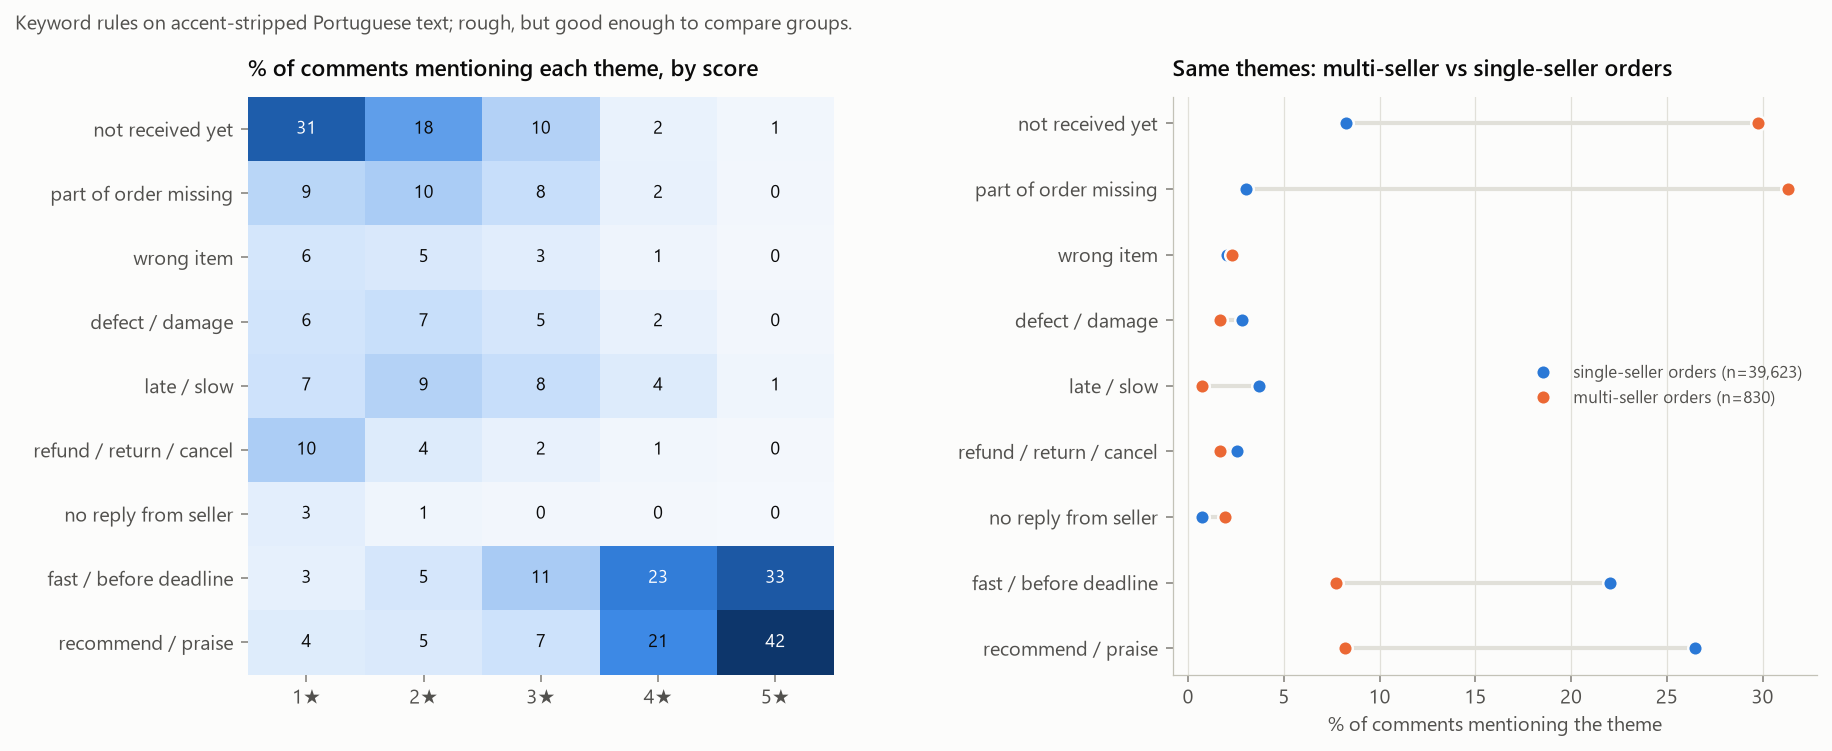
\includegraphics[width=\linewidth]{eda/15_text_themes}
  \caption{Chủ đề trong bình luận đánh giá}
  \label{fig:eda-themes}
\end{figure}

So sánh bình luận tiêu cực của đơn trễ và đơn đúng hạn làm rõ khác biệt về bản chất. Trong 2\,747 bình luận 1--2 sao của đơn trễ, 52,4\% nói chưa nhận được hàng và chỉ 2,0\% nói hàng sai, khác mô tả, lỗi hoặc vỡ. Trong 6\,487 bình luận 1--2 sao của đơn đúng hạn, hai tỉ lệ này lần lượt là 13,9\% và 17,9\%, và 20,3\% nói chỉ nhận được một phần đơn; riêng đơn đúng hạn có từ hai người bán, tỉ lệ nói thiếu một phần lên 51,9\%. Có 78,3\% đánh giá thấp của đơn đúng hạn kèm bình luận. Nói cách khác, khách phàn nàn về đơn trễ vì hàng \emph{chưa đến}, còn khách phàn nàn về đơn đúng hạn vì \emph{thứ đã đến} bị thiếu, sai, hỏng hoặc kém chất lượng. Không vấn đề nào trong số này lộ ra qua chênh lệch giữa ngày giao và ngày dự kiến.

\subsection{Hàm ý cho thiết kế đặc trưng}\label{subsec:eda-implications}

Kết quả khám phá dữ liệu định hướng trực tiếp các nhóm đặc trưng ở Bảng~\ref{tab:features}. Tín hiệu mạnh nhất trong nhóm đúng hạn đến từ cấu trúc đơn, nên số người bán, số danh mục, số sản phẩm, các cờ nhiều item, nhiều người bán, nhiều danh mục và chỉ số tập trung Herfindahl--Hirschman được tách thành ba nhóm riêng. Do Olist chỉ có một mốc giao cho mỗi đơn, các đặc trưng này đóng vai trò đại diện gián tiếp cho việc giao thiếu hoặc tách kiện mà bình luận phản ánh. Thời gian giao thực tế, thời gian vận chuyển và khoảng dư so với ngày dự kiến được giữ trong nhóm cơ sở vì đơn chờ lâu vẫn có rủi ro cao dù kịp hạn; quan hệ chữ U của khoảng dư là thêm một lý do để ưu tiên mô hình cây.

Lịch sử đánh giá của người bán và danh mục, cùng nhóm tốc độ và độ biến động của người bán, khai thác tín hiệu từ người bán bàn giao trễ và người bán có tiền sử bị đánh giá thấp; cả hai đều phải tính với ranh giới thời gian chặt như ở Hình~\ref{fig:leakage-timeline}. Danh mục được giữ ở dạng biến phân loại kèm nhóm ``thiếu''. Các nhóm hình thái sản phẩm và độ đầy đủ nội dung nhắm đến các lời phàn nàn về hư hỏng và hàng khác mô tả. Phí vận chuyển, giá trị đơn và thanh toán chỉ cho tín hiệu yếu ở bước khám phá; chúng vẫn nằm trong nhóm cơ sở, nhưng không nên kỳ vọng đóng góp lớn từ riêng các biến này. Ngược lại, văn bản, tiêu đề, thời điểm tạo và thời điểm trả lời đánh giá bị loại khỏi tập đặc trưng, vì đó là thông tin chỉ có sau khi nhãn đã hình thành. Mục~\ref{sec:analysis-eda} kiểm tra lại các kỳ vọng này bằng kết quả thực nghiệm.

% =====================================================================
\section{Kết quả đạt được}\label{sec:results}

\subsection{Các thành phần đã hoàn thành}\label{subsec:res-summary}

Quá trình thực nghiệm tạo ra một pipeline đầy đủ từ dữ liệu thô đến điểm rủi ro mức đơn, cùng một mô hình được chọn theo quy tắc đã định trước ở mục~\ref{sec:models}. Bảng~\ref{tab:res-summary} tóm tắt các thành phần chính. Mô hình giữ lại là rừng ngẫu nhiên 200 cây, độ sâu tối đa 8, tối thiểu 5 mẫu mỗi lá, trọng số lớp cân bằng tính lại trên từng mẫu bootstrap, huấn luyện ở chế độ order-weight, tức mỗi item có trọng số bằng nghịch đảo số item trong đơn. Tập đặc trưng cuối cùng gồm 61 đặc trưng thuộc bảy nhóm ở Bảng~\ref{tab:features}, là kết quả của mười giai đoạn thử nghiệm có kiểm soát. Chín giai đoạn đầu mỗi lần thêm một nhóm đặc trưng ứng viên và chỉ giữ nhóm đó khi nó cải thiện PR-AUC mức đơn trung bình qua ba fold rolling-origin; giai đoạn cuối kiểm tra lại các nhóm đã giữ bằng cách bỏ từng nhóm một.

\begin{table}[htbp]\centering\small
\caption{Tóm tắt kết quả thực nghiệm (kết quả phát triển, mang tính thăm dò)}\label{tab:res-summary}
\begin{tabular}{p{3.6cm}p{9.9cm}}
\toprule
Thành phần & Kết quả \\
\midrule
Dữ liệu mô hình hóa & Snapshot đóng băng 85\,425 đơn, 97\,884 item \\
Tập đặc trưng & 61 đặc trưng, 7 nhóm: nhóm cơ sở và các nhóm từ 3 giai đoạn thử nghiệm được giữ \\
Mô hình giữ lại & Rừng ngẫu nhiên, độ sâu 8, lá tối thiểu 5, chế độ order-weight \\
Hiệu chỉnh & Sigmoid; Brier mức item trên phân vùng so sánh giảm từ 0,2203 xuống 0,1049 \\
Ngưỡng ưu tiên & Top 5\% đơn là \textsc{Cao}, top 20\% là \textsc{Trung bình} trở lên \\
PR-AUC mức đơn & 0,1465 (trung bình ba fold; mô hình ban đầu 0,1363) \\
Recall@5\% & 0,1212 (trung bình ba fold; mốc chọn ngẫu nhiên 0,05) \\
Brier mức đơn chưa hiệu chỉnh & 0,1907 (trung bình ba fold; mô hình ban đầu 0,2018) \\
\bottomrule
\end{tabular}
\end{table}

So với mô hình ban đầu cùng họ và cùng chế độ huấn luyện nhưng chỉ dùng nhóm đặc trưng cơ sở, PR-AUC mức đơn trung bình tăng 0,0102 (khoảng 7,5\%) và Brier score giảm 0,0112. Mục tiêu dừng PR-AUC 0,25 của kế hoạch cải thiện không đạt; kế hoạch kết thúc khi các thử nghiệm tiếp theo, kể cả ba cấu hình CatBoost chạy trên GPU và chế độ gộp item thành đơn trước khi huấn luyện, không vượt được mô hình đã giữ trên chỉ số chính.

\subsection{Hệ thống hỗ trợ vận hành}\label{sec:system-api}

Bên cạnh mô hình, đề tài hoàn thành một ứng dụng đưa điểm rủi ro vào quy trình chăm sóc khách hàng (kiến trúc ở Hình~
ef{fig:arch}).

Luồng ngoại tuyến nạp dữ liệu, tạo đặc trưng, huấn luyện và chấm điểm theo lô. Luồng trực tuyến chỉ đọc snapshot điểm đã được ghi để tạo hàng đợi, phân công và ghi nhận xử lý. Việc tách hai luồng loại trừ một rủi ro cơ bản: một thao tác trên giao diện không được làm thay đổi dữ liệu, ngưỡng hay phiên bản mô hình.

PostgreSQL lưu kho dữ liệu Bronze/Silver/Gold, schema \texttt{ml} lưu release, snapshot và ngưỡng, còn schema \texttt{app} lưu case và lịch sử xử lý. Snapshot là điểm nối giữa hai phần. Nó ghi score, phiên bản model, phiên bản ngưỡng, thời điểm chấm điểm và nguồn dữ liệu. Case có thể thay đổi người phụ trách hoặc trạng thái; score và mức rủi ro của snapshot không được sửa qua API. Vì vậy, một quyết định sau này luôn có thể được đối chiếu với thông tin đã có khi hàng đợi được tạo.

API dùng Bearer JWT, còn kiểm soát quyền được thực hiện ở backend. \texttt{SPECIALIST} xem hàng đợi, nhận các case thấp/trung bình hợp lệ và ghi liên lạc. \texttt{MANAGER} phân công case HIGH, mở lại case, đặt quyết định, xem audit và thay đổi tham số. Sự phân vai này không chứng minh hiệu quả CSKH; nó chỉ xác định ai được phép thực hiện bước nào trong quy trình.

Case đi qua \texttt{PENDING}, \texttt{IN\_PROGRESS}, \texttt{COMPLETED} hoặc \texttt{SKIPPED}. Specialist không thể nhận case đã có người xử lý, case HIGH hoặc case vượt năng lực. Khi case được đóng hoặc mở lại, backend tạo và kiểm tra giao dịch thay vì để giao diện tự suy diễn trạng thái. Contact, comment, decision và parameter version được ghi thêm thay vì ghi đè; audit event ghi lại thay đổi workflow. Các quy tắc này phục vụ khả năng kiểm tra, không phải là một lớp trang trí cho giao diện.

Các endpoint dưới tiền tố \texttt{/api/v1} phản ánh các ranh giới trên: \texttt{/auth} cho phiên làm việc; \texttt{/orders} cho hàng đợi và nhận case; \texttt{/contacts}, \texttt{/comments}, \texttt{/decisions} cho bằng chứng xử lý; \texttt{/dashboard}, \texttt{/audit-events} và \texttt{/parameters} cho giám sát. Hàng đợi mặc định sắp theo score giảm dần, tiếp đến SLA và thời gian chờ. Do đó score chỉ quyết định thứ tự cần xem xét, không tự gắn nhãn khách hàng hoặc tự gửi liên hệ.

\subsection{Phạm vi của bằng chứng}\label{subsec:res-scope}

Mọi số liệu mô hình trong chương này là kết quả phát triển, tính trên ba fold rolling-origin bên trong phân vùng huấn luyện, và mang tính thăm dò. Phân vùng test lịch sử đã bị lộ trong quá trình phát triển, nên quy trình hoàn tất không cho phép chấm điểm trên phân vùng đó; muốn có kết luận xác nhận cần một tập kiểm tra mới, được niêm phong trước khi xem xét. Do chưa có lần chạy hoàn tất nào, các kết quả sau đây \emph{chưa} được tính, gồm chỉ số trên tập test, khoảng tin cậy bootstrap theo cụm đơn, đường cong precision--recall và đường cong hiệu chỉnh, kết quả ở các ngân sách 10\% và 20\%, mốc so sánh theo giá trị đơn, và giá trị SHAP. Báo cáo thực nghiệm cũng không ghi ROC-AUC theo fold, Brier mức item theo fold và tỉ lệ dương của từng đoạn kiểm định; nhóm không suy ra các đại lượng này.

Các con số dưới đây vì vậy trả lời câu hỏi ``trong giai đoạn phát triển, mô hình xếp hạng và ước lượng xác suất tốt đến đâu, và mức đó có ổn định qua thời gian không'', chứ chưa phải ước lượng cuối cùng về hiệu năng khi triển khai.

% =====================================================================
\section{Bảng biểu và số liệu}\label{sec:tables}

\subsection{Hiệu năng của mô hình giữ lại theo fold}\label{subsec:tab-folds}

Bảng~\ref{tab:res-folds} trình bày bốn chỉ số của mô hình giữ lại trên từng fold. Cột cuối là hệ số nâng tại ngân sách 5\%, tức Recall@5\% chia cho 0,05, mức recall kỳ vọng khi chọn ngẫu nhiên (công thức~\eqref{eq:th-recallk}). Ba fold có đoạn kiểm định lần lượt bắt đầu ngày 1/6/2017, 18/7/2017 và 24/8/2017 (Hình~\ref{fig:temporal-folds}).

\begin{table}[htbp]\centering\small
\caption{Kết quả của mô hình giữ lại theo fold rolling-origin (rừng ngẫu nhiên, order-weight, chưa hiệu chỉnh)}\label{tab:res-folds}
\begin{tabular}{crrrrr}
\toprule
Fold & PR-AUC item & PR-AUC đơn & Brier đơn & Recall@5\% & Hệ số nâng \\
\midrule
1 & 0,1538 & 0,1425 & 0,1883 & 0,1141 & 2,28 \\
2 & 0,1883 & 0,1507 & 0,1899 & 0,1309 & 2,62 \\
3 & 0,1860 & 0,1463 & 0,1938 & 0,1187 & 2,37 \\
\midrule
Trung bình & 0,1760 & 0,1465 & 0,1907 & 0,1212 & 2,42 \\
\bottomrule
\end{tabular}
\end{table}

Hình~\ref{fig:res-folds} so sánh mô hình giữ lại với mô hình ban đầu trên cùng ba fold. Mô hình giữ lại tốt hơn ở cả ba fold, theo cả PR-AUC mức đơn lẫn Recall@5\%. Mức cải thiện PR-AUC lần lượt là 0,0120, 0,0060 và 0,0125; Recall@5\% tăng 0,0121, 0,0123 và 0,0158.

\begin{figure}[htbp]\centering
\begin{tikzpicture}[x=1cm,y=25cm,font=\footnotesize]
  % y: 0,16 = 4 cm
  \foreach \ox/\ttl in {0/{PR-AUC mức đơn},6.6/{Recall@5\%}} {
    \begin{scope}[xshift=\ox cm]
      \draw (0,0) -- (5.4,0);
      \draw (0,0) -- (0,0.165);
      \foreach \t/\l in {0/0,0.05/{0,05},0.10/{0,10},0.15/{0,15}} {
        \draw (-0.08,\t) -- (0,\t) node[left,font=\scriptsize]{\l};
        \draw[gray!25] (0,\t) -- (5.4,\t);
      }
      \node[font=\small] at (2.7,0.185) {\ttl};
      \foreach \k in {1,2,3} \node[below,font=\scriptsize] at (1.6*\k-0.5,0) {Fold \k};
    \end{scope}
  }
  % PR-AUC mức đơn: ban đầu / giữ lại
  \foreach \k/\a/\b/\la/\lb in {1/0.1305/0.1425/{0,131}/{0,143},2/0.1447/0.1507/{0,145}/{0,151},3/0.1338/0.1463/{0,134}/{0,146}} {
    \fill[gray!45] (1.6*\k-1.0,0) rectangle (1.6*\k-0.52,\a);
    \fill[blue!55] (1.6*\k-0.48,0) rectangle (1.6*\k,\b);
    \node[above,font=\tiny] at (1.6*\k-0.76,\a) {\la};
    \node[above,font=\tiny] at (1.6*\k-0.24,\b) {\lb};
  }
  % Recall@5%: ban đầu / giữ lại
  \begin{scope}[xshift=6.6cm]
    \foreach \k/\a/\b/\la/\lb in {1/0.1019/0.1141/{0,102}/{0,114},2/0.1185/0.1309/{0,119}/{0,131},3/0.1029/0.1187/{0,103}/{0,119}} {
      \fill[gray!45] (1.6*\k-1.0,0) rectangle (1.6*\k-0.52,\a);
      \fill[blue!55] (1.6*\k-0.48,0) rectangle (1.6*\k,\b);
      \node[above,font=\tiny] at (1.6*\k-0.76,\a) {\la};
      \node[above,font=\tiny] at (1.6*\k-0.24,\b) {\lb};
    }
    \draw[red!70!black,dashed] (0,0.05) -- (5.4,0.05);
  \end{scope}
  % chú giải
  \fill[gray!45] (0.4,-0.03) rectangle (0.7,-0.022); \node[right,font=\scriptsize] at (0.7,-0.026) {Mô hình ban đầu (chỉ nhóm cơ sở)};
  \fill[blue!55] (5.8,-0.03) rectangle (6.1,-0.022); \node[right,font=\scriptsize] at (6.1,-0.026) {Mô hình giữ lại};
  \draw[red!70!black,dashed] (8.7,-0.026) -- (9.3,-0.026); \node[right,font=\scriptsize] at (9.3,-0.026) {Chọn ngẫu nhiên 5\%};
\end{tikzpicture}
\caption{PR-AUC mức đơn và Recall@5\% theo fold}
\label{fig:res-folds}
\end{figure}

\subsection{Đóng góp của các nhóm đặc trưng}\label{subsec:tab-features}

Bảng~\ref{tab:res-phases} liệt kê chín giai đoạn thêm nhóm đặc trưng. Ba nhóm được giữ được thêm nối tiếp nhau, nên PR-AUC tăng từ 0,1363 lên 0,1407 sau giai đoạn 2, lên 0,1445 sau giai đoạn 4 và lên 0,1465 sau giai đoạn 6. Sáu nhóm còn lại bị loại vì mức cải thiện tốt nhất không vượt ngưỡng hoặc làm giảm chỉ số. Cả ba nhóm được giữ đều cải thiện PR-AUC ở từng fold riêng lẻ, không chỉ ở giá trị trung bình.

\begin{table}[htbp]\centering\small
\caption{Kết quả các giai đoạn thử nghiệm nhóm đặc trưng (thay đổi PR-AUC mức đơn trung bình ba fold so với tập đang giữ)}\label{tab:res-phases}
\begin{tabular}{clrl}
\toprule
Giai đoạn & Nhóm đặc trưng ứng viên & Thay đổi PR-AUC & Quyết định \\
\midrule
1 & Lịch sử nhãn của người bán và danh mục (làm trơn) & $+0{,}0015$ (tốt nhất) & Loại \\
2 & Tốc độ và độ biến động vận hành của người bán & $+0{,}0044$ & Giữ \\
3 & Địa lý và tuyến vận chuyển & $-0{,}0024$ (tốt nhất) & Loại \\
4 & Cấu trúc đơn: số lượng, tỉ lệ, mức độ tập trung & $+0{,}0038$ & Giữ \\
5 & Hành vi thanh toán & $+0{,}0006$ (tốt nhất) & Loại \\
6 & Hình thái sản phẩm và độ đầy đủ nội dung & $+0{,}0020$ & Giữ \\
7 & Lịch và khối lượng đơn trước đó & $-0{,}0004$ (tốt nhất) & Loại \\
8 & Cờ chất lượng dữ liệu & $-0{,}0024$ & Loại \\
9 & Tương tác có kiểm soát & $-0{,}0005$ & Loại \\
\bottomrule
\end{tabular}
\end{table}

Giai đoạn 10 kiểm tra lại ba nhóm được giữ bằng cách bỏ từng nhóm một (leave-one-group-out). Bảng~\ref{tab:res-loo} cho thấy bỏ nhóm nào cũng làm PR-AUC giảm ít nhất bằng dung sai 0,002 đặt trước, nên tập đặc trưng rút gọn trùng với tập đầy đủ. Nhóm hình thái và nội dung sản phẩm nằm đúng ở ranh giới này. Cột cuối là PR-AUC mức đơn trên phân vùng lựa chọn mô hình (Bảng~\ref{tab:split}), một tập kiểm định đơn lẻ được báo cáo như bằng chứng phụ.

\begin{table}[htbp]\centering\small
\caption{Bỏ từng nhóm đặc trưng khỏi tập giữ lại (trung bình ba fold, trừ cột cuối)}\label{tab:res-loo}
\begin{tabular}{p{5.6cm}rrrr}
\toprule
Tập đặc trưng & PR-AUC đơn & Thay đổi & Brier đơn & PR-AUC lựa chọn \\
\midrule
Đầy đủ (7 nhóm) & 0,1465 & -- & 0,1907 & 0,2108 \\
Bỏ tốc độ và độ biến động người bán & 0,1424 & $-0{,}0042$ & 0,1956 & 0,2113 \\
Bỏ cấu trúc đơn & 0,1415 & $-0{,}0050$ & 0,1902 & 0,1999 \\
Bỏ hình thái và nội dung sản phẩm & 0,1445 & $-0{,}0020$ & 0,1946 & 0,2185 \\
\bottomrule
\end{tabular}
\end{table}

\subsection{So sánh với các cấu hình CatBoost}\label{subsec:tab-catboost}

Ba cấu hình CatBoost xử lý biến phân loại trực tiếp được chạy trên cùng tập đặc trưng và cùng ba fold (Bảng~\ref{tab:res-catboost}). Kho lưu trữ chỉ giữ số liệu theo fold của rừng ngẫu nhiên và ba cấu hình này; số liệu của mô hình tỉ lệ nền, hồi quy logistic và HistGradientBoosting không còn, nên bảng không phải là bảng xếp hạng đầy đủ năm họ mô hình đã khai báo ở mục~\ref{sec:models}.

\begin{table}[htbp]\centering\small
\caption{Rừng ngẫu nhiên giữ lại so với ba cấu hình CatBoost (chế độ order-weight, cùng tập đặc trưng)}\label{tab:res-catboost}
\begin{tabular}{lrrrr}
\toprule
& \multicolumn{3}{c}{Trung bình ba fold} & Phân vùng lựa chọn \\
\cmidrule(lr){2-4}\cmidrule(lr){5-5}
Mô hình & PR-AUC đơn & Brier đơn & Recall@5\% & PR-AUC đơn \\
\midrule
Rừng ngẫu nhiên, độ sâu 8, lá 5 & \textbf{0,1465} & 0,1907 & 0,1212 & 0,2108 \\
CatBoost, độ sâu 6, L2 $=8$ & 0,1458 & 0,1681 & \textbf{0,1319} & \textbf{0,2239} \\
CatBoost, độ sâu 8 & 0,1357 & 0,1468 & 0,1229 & 0,2004 \\
CatBoost, độ sâu 10, L2 $=8$ & 0,1374 & \textbf{0,1310} & 0,1180 & 0,1986 \\
\bottomrule
\end{tabular}
\end{table}

Theo thứ tự ưu tiên đã định, rừng ngẫu nhiên được giữ vì có PR-AUC trung bình ba fold cao nhất, dù cấu hình CatBoost độ sâu 6 cao hơn trên phân vùng lựa chọn mô hình và ở Recall@5\%. Không có cấu hình nào đạt mức cải thiện ổn định 0,005 cần thiết để ghép thành mô hình kết hợp.

\subsection{Hiệu chỉnh xác suất và ngưỡng ưu tiên}\label{subsec:tab-calibration}

Mô hình giữ lại được huấn luyện lại trên phân vùng huấn luyện và lựa chọn, hai bộ hiệu chỉnh được fit trên phân vùng fit hiệu chỉnh, rồi cả ba phương án được so sánh bằng Brier score trên phân vùng so sánh hiệu chỉnh (Bảng~\ref{tab:res-calibration}). Brier ở bước này được tính trên xác suất mức item, không có trọng số, nên không so sánh trực tiếp được với Brier mức đơn ở Bảng~\ref{tab:res-folds}. Dòng cuối là dự đoán hằng số bằng tỉ lệ dương mức item của phân vùng so sánh (13,80\%), có Brier bằng $\pi(1-\pi)$, được tính thêm làm mốc tham chiếu.

\begin{table}[htbp]\centering\small
\caption{Brier score mức item trên phân vùng so sánh hiệu chỉnh (2/2018--3/2018)}\label{tab:res-calibration}
\begin{tabular}{lr}
\toprule
Phương án & Brier \\
\midrule
Không hiệu chỉnh & 0,2203 \\
Isotonic & 0,1057 \\
Sigmoid (được chọn) & \textbf{0,1049} \\
\midrule
\emph{Tham chiếu:} dự đoán hằng số $\pi = 0{,}138$ & 0,1189 \\
\bottomrule
\end{tabular}
\end{table}

Với ứng viên CatBoost độ sâu 6, bước hiệu chỉnh cũng chọn sigmoid, với Brier 0,1071 trên cùng phân vùng. Ngưỡng ưu tiên theo chính sách phát triển là 5\% đơn có điểm cao nhất cho mức \textsc{Cao} và 20\% cho mức \textsc{Trung bình} trở lên. Trong một lần chạy rừng ngẫu nhiên trước đó, hai ngưỡng này tương ứng với điểm 0,2858 và 0,1119; đây là ngưỡng chọn trên phân vùng chọn ngưỡng, chưa phải kết quả vận hành trên tập test.

% =====================================================================
\section{Phân tích và đánh giá}\label{sec:results-analysis}

Mục này đánh giá các kết quả ở mục~\ref{sec:tables} theo bốn câu hỏi, gồm mô hình xếp hạng tốt hơn ngẫu nhiên đến mức nào, mức đó có ổn định qua thời gian không, xác suất có đáng tin không, và kết quả có nhất quán với những gì dữ liệu cho thấy ở bước khám phá không.

\subsection{Khả năng xếp hạng so với mốc ngẫu nhiên}\label{sec:analysis-ranking}

PR-AUC chỉ có nghĩa khi đặt cạnh tỉ lệ dương, vì một mô hình xếp hạng ngẫu nhiên có PR-AUC xấp xỉ tỉ lệ dương (mục~\ref{sec:th-metrics}). Báo cáo thực nghiệm không ghi tỉ lệ dương mức đơn của từng đoạn kiểm định. Nếu tỉ lệ này nằm trong khoảng 8,86--10,53\% như ở các phân vùng phát triển (mục~\ref{subsec:eda-labels}), PR-AUC mức đơn trung bình 0,1465 gấp khoảng 1,4 đến 1,65 lần mốc ngẫu nhiên. Mô hình vì thế học được tín hiệu thật, nhưng tín hiệu đó yếu, vì phần lớn các đơn có điểm cao vẫn là đơn không bị đánh giá thấp.

Ở mức vận hành, Recall@5\% trung bình 0,1212 cho hệ số nâng 2,42, dao động 2,28--2,62 giữa các fold. Nếu bộ phận chăm sóc khách hàng chỉ liên hệ được 5\% số đơn giao đúng hạn, danh sách theo mô hình chứa khoảng 12\% số đơn sẽ bị đánh giá thấp, so với 5\% khi chọn ngẫu nhiên. Từ công thức~\eqref{eq:th-recallk}, $\mathrm{Precision@}b = \mathrm{Recall@}b \cdot \pi / b$; với $\pi$ trong khoảng 8,86--10,53\% như trên, khoảng 21--26\% số đơn được gắn mức \textsc{Cao} thực sự bị đánh giá thấp, tức chừng một trong bốn hoặc năm đơn, so với khoảng một trong mười đơn nếu chọn ngẫu nhiên. Đây là ước tính suy ra, chưa phải số đo trực tiếp.

PR-AUC mức item (0,1760) cao hơn mức đơn (0,1465), nhưng chênh lệch này chủ yếu đến từ mốc so sánh chứ không phải từ chất lượng xếp hạng. Trong quần thể nghiên cứu, tỉ lệ dương mức item là 11,41\%, cao hơn mức đơn 9,21\%, vì đơn nhiều sản phẩm vừa có tỉ lệ đánh giá thấp cao hơn vừa đóng góp nhiều dòng hơn. Chia cho tỉ lệ dương tương ứng của quần thể, cả hai chỉ số đều ở khoảng 1,5--1,6 lần mốc ngẫu nhiên. Ngoài ra, các item trong cùng một đơn dương có đặc trưng mức đơn giống nhau và cùng nhãn, nên PR-AUC mức item được lợi từ việc đếm lặp. Vì đơn hàng là đơn vị nhân viên xử lý, PR-AUC mức đơn mới là chỉ số phản ánh giá trị vận hành, đúng như lựa chọn ở mục~\ref{sec:eval}.

\subsection{Độ ổn định qua thời gian và lựa chọn mô hình}\label{sec:analysis-stability}

PR-AUC mức đơn của mô hình giữ lại dao động từ 0,1425 đến 0,1507 giữa ba fold, với độ lệch chuẩn khoảng 0,004. Con số này cho một thang đo để đọc Bảng~\ref{tab:res-phases}. Mỗi nhóm đặc trưng được giữ chỉ cải thiện 0,0020--0,0044, tức xấp xỉ một độ lệch chuẩn giữa các fold. Một mức cải thiện trung bình cỡ đó có thể là nhiễu, và đó là lý do quyết định giữ nhóm còn dựa vào việc nhóm có cải thiện ở từng fold hay không. Mức cải thiện cộng dồn 0,0102 bằng khoảng 2,5 lần độ lệch chuẩn và xuất hiện ở cả ba fold (Hình~\ref{fig:res-folds}), nên đáng tin hơn bất kỳ bước riêng lẻ nào. Fold 1 có PR-AUC mức item thấp nhất (0,1538); đây cũng là fold học trên ít dữ liệu nhất, phù hợp với nhận xét ở mục~\ref{sec:th-temporal}, dù với ba fold thì chưa thể tách tác động của cỡ mẫu khỏi đặc điểm của từng giai đoạn.

Cùng thang đo đó cho thấy rừng ngẫu nhiên và CatBoost độ sâu 6 gần như ngang nhau. Chênh lệch PR-AUC ba fold giữa hai mô hình chỉ là 0,0007, nhỏ hơn nhiều so với độ lệch chuẩn giữa các fold. Ở Recall@5\%, CatBoost độ sâu 6 cao hơn 0,0107 và không kém rừng ngẫu nhiên ở fold nào (0,1408, 0,1309 và 0,1240 so với 0,1141, 0,1309 và 0,1187). Quy tắc chọn theo PR-AUC đã được cố định trước khi chạy và được áp dụng đúng; tuy vậy, kết quả này cho thấy nếu ngân sách 5\% là ràng buộc vận hành chính, Recall@5\% có lý do để trở thành tiêu chí phụ trong lần lựa chọn sau. Trên phân vùng lựa chọn mô hình, thứ hạng hai mô hình đảo ngược (0,2239 so với 0,2108); ý nghĩa của sự đảo ngược này đối với cách đánh giá được bàn ở mục~\ref{sec:disc-findings}.

Kết quả bỏ từng nhóm cũng cho thấy giới hạn của một tập kiểm định đơn lẻ. Bỏ nhóm hình thái và nội dung sản phẩm làm PR-AUC ba fold giảm 0,0020 nhưng làm PR-AUC trên phân vùng lựa chọn \emph{tăng} từ 0,2108 lên 0,2185 (Bảng~\ref{tab:res-loo}). Hai nguồn bằng chứng chỉ ra hai hướng ngược nhau, và nhóm này được giữ có điều kiện theo chỉ số chính. Ngược lại, nhóm cấu trúc đơn làm giảm cả hai chỉ số khi bị bỏ, nên là nhóm có bằng chứng vững nhất.

\subsection{Độ tin cậy của xác suất}\label{sec:analysis-calibration}

Trước hiệu chỉnh, xác suất của mô hình kém tin cậy. Brier mức đơn trung bình ba fold là 0,1907, trong khi một dự đoán hằng số bằng tỉ lệ dương mức đơn 8,86--10,53\% cho Brier $\pi(1-\pi)$ khoảng 0,081--0,094. Trên phân vùng so sánh hiệu chỉnh, Brier mức item của mô hình gốc là 0,2203, cao gần gấp đôi mốc hằng số 0,1189. Đây đúng là hệ quả mà mục~\ref{sec:th-trees} đã dự đoán. Trọng số lớp cân bằng làm tỉ lệ dương hiệu dụng trong các lá cao hơn thực tế, nên xác suất bị đẩy lên một cách có hệ thống, phù hợp với kết quả của \textcite{vandengoorbergh2022}. Ba cấu hình CatBoost có Brier ba fold thấp hơn (0,1310--0,1681), cho thấy mức méo phụ thuộc vào mô hình nhưng không biến mất.

Hiệu chỉnh sửa được phần lớn độ lệch này. Sigmoid giảm Brier mức item từ 0,2203 xuống 0,1049, tức giảm 52\%, và đưa mô hình xuống dưới mốc hằng số 0,1189 khoảng 12\%. Isotonic cho kết quả gần như bằng (0,1057). Khi tập fit hiệu chỉnh có 11\,759 đơn, nguy cơ quá khớp của isotonic mà \textcite{niculescumizil2005} cảnh báo không thể hiện rõ; sigmoid được chọn vì Brier thấp hơn và vì nó giữ nguyên hoàn toàn thứ tự xếp hạng (mục~\ref{sec:th-calibration}). Rừng ngẫu nhiên sau hiệu chỉnh cũng nhỉnh hơn CatBoost độ sâu 6 sau hiệu chỉnh (0,1049 so với 0,1071).

Kết quả này còn một khoảng trống. Brier sau hiệu chỉnh đã có ở mức item, nhưng Brier mức đơn sau hiệu chỉnh và sau khi gộp bằng max-v1 chưa được báo cáo. Mục~\ref{sec:th-aggregation} đã chỉ ra rằng xác suất item hiệu chỉnh tốt không bảo đảm điểm đơn hiệu chỉnh tốt, vì giá trị lớn nhất của nhiều xác suất có xu hướng cao hơn từng xác suất. Do đó, điểm đơn hiển thị trên giao diện nên được đọc như thứ hạng ưu tiên hơn là xác suất chính xác, cho đến khi Brier mức đơn sau hiệu chỉnh được đo.

\subsection{Đối chiếu với kết quả khám phá dữ liệu}\label{sec:analysis-eda}

Kết quả chọn đặc trưng khớp với các tín hiệu tìm thấy ở mục~\ref{subsec:eda-ontime}. Nhóm cấu trúc đơn, nơi bước khám phá ghi nhận khác biệt lớn nhất (45,7\% ở đơn hai người bán, 31,9\% ở đơn từ bốn item), là nhóm được giữ có đóng góp lớn nhất khi bỏ ra ($-0{,}0050$). Nhóm vận hành của người bán tương ứng với tín hiệu bàn giao vận chuyển sau hạn (13,6\% so với 8,9\%) và được giữ với mức giảm $-0{,}0042$ khi bỏ. Nhóm sản phẩm tương ứng với khác biệt giữa các danh mục và tỉ lệ cao ở item thiếu danh mục. Ở chiều ngược lại, các yếu tố gần như phẳng ở bước khám phá đều bị loại khi thử nghiệm. Thanh toán (8,5--10,5\% theo phương thức) chỉ cải thiện tốt nhất 0,0006, còn địa lý (8,6--11,1\% theo bang) làm giảm PR-AUC.

Ngoại lệ đáng chú ý là lịch sử nhãn. Bước khám phá cho thấy người bán có tiền sử nhiều đánh giá thấp tạo ra tỉ lệ đánh giá thấp gấp gần ba lần (18,4\% so với 6,5\%), nhưng nhóm lịch sử nhãn làm trơn ở giai đoạn 1 chỉ cải thiện tốt nhất 0,0015 và bị loại. Hai kết quả này không mâu thuẫn, bởi nhóm cơ sở đã có số đánh giá trước đó và điểm trung bình trước đó của người bán và danh mục, nên các phép mã hóa mới chủ yếu lặp lại thông tin đã có. Ý nghĩa của việc đặc trưng vận hành vượt lịch sử đánh giá được thảo luận ở mục~\ref{sec:disc-findings}.

Bước khám phá cũng cho phép đánh giá một phần thiên lệch của luật max-v1. Công thức~\eqref{eq:th-maxbias} dự đoán max-v1 nâng điểm đơn nhiều item ngay cả khi từng item không rủi ro hơn. Trong quần thể nghiên cứu, đơn nhiều item thực sự rủi ro hơn, với tỉ lệ 23,2--31,9\% so với 7,5\% ở đơn một item (Bảng~\ref{tab:eda-segments}). Thiên lệch của max-v1 vì vậy cùng chiều với rủi ro thật, nên nó ít có khả năng đẩy sai đơn lên đầu danh sách. Tuy nhiên, chưa thể biết max-v1 nâng điểm các đơn này vừa đủ hay quá mức, vì dự đoán mức đơn theo số item chưa được lưu lại để kiểm tra.

\subsection{Đánh giá tổng hợp}\label{sec:analysis-summary}

Trong phạm vi bằng chứng phát triển, kết quả đáp ứng hai tiêu chí tối thiểu của mục~\ref{sec:eval}. Mô hình xếp hạng tốt hơn ngẫu nhiên ở cả mức đơn lẫn ngân sách 5\%, và mức vượt đó xuất hiện ở cả ba fold chứ không chỉ ở giá trị trung bình. Xác suất sau hiệu chỉnh tốt hơn dự đoán hằng số ở mức item. Ba giới hạn ảnh hưởng trực tiếp đến cách đọc các con số. Thứ nhất, tín hiệu còn yếu, khi PR-AUC chỉ khoảng 1,4--1,65 lần mốc ngẫu nhiên, và khoảng 88\% số đơn bị đánh giá thấp nằm ngoài nhóm 5\% đầu danh sách. Thứ hai, độ chính xác của phép lựa chọn bị giới hạn bởi ba fold; phần lớn chênh lệch giữa các phương án cạnh tranh nhỏ hơn độ dao động giữa các fold. Thứ ba, các kết quả chưa được xác nhận trên tập test niêm phong và chưa có mốc so sánh theo giá trị đơn. Chương~\ref{ch:discussion} đặt các kết quả này cạnh mục tiêu ban đầu và bàn về nguyên nhân của mức tín hiệu thấp; mục tiếp theo trình bày cách điểm rủi ro được dùng trong ứng dụng.

Vì vậy, bước tiếp theo không phải tiếp tục tô đậm metric hiện có. Cần khóa một replacement holdout chưa được quan sát, chốt model, calibration, aggregation và ngưỡng trước khi đánh giá, rồi xuất metric kèm khoảng tin cậy và artefact dự đoán. Chỉ khi đó mới có thể chuyển từ bằng chứng phát triển sang một kết luận xác nhận.

% Chương 4 — phần giao diện/demo (Trúc). Ghép vào cuối \chapter{Kết quả và phân tích}.
% Nguồn: BA/*.md, reports/P13-full-flow-audit-2026-10-31.md, SERVER_CONTEXT/chapter4_evidence.md (nhánh thesis),
% ảnh chụp 05/11/2026 từ stack Docker nhánh dev (commit 1a8a767).
% Phần này trả lời câu hỏi: điểm số của mô hình được đưa vào quy trình chăm sóc khách hàng như thế nào.
% Chia việc Ch.4: Quân (EDA, dữ liệu) · Trung (hệ thống/API) · Huy (bảng metric) · Trúc (giao diện/demo).
% Không lặp kiến trúc/API (phần Trung) và kết quả kiểm thử web (để ở báo cáo kiểm thử, không đưa vào khóa luận ML).

\section{Ứng dụng điểm rủi ro vào quy trình chăm sóc khách hàng}\label{sec:demo}

Một điểm rủi ro chỉ tạo ra giá trị khi nó thay đổi việc nhân viên làm tiếp theo. Mục này trình bày cách đầu ra của luồng học máy ở Chương~\ref{ch:method} được đưa vào ứng dụng vận hành: điểm số biến thành thứ tự ưu tiên ra sao, người dùng đọc và diễn giải điểm số ở đâu, và hệ thống ghi lại những gì để đánh giá mô hình về sau. Hai phần minh họa cuối mục cho thấy luật tổng hợp và ngưỡng ưu tiên làm thay đổi danh sách đơn ra sao. Dữ liệu đầu vào và kiến trúc hệ thống được trình bày ở các mục khác của chương này nên không nhắc lại.

Cần nói rõ ngay từ đầu: điểm số trong bản demo \emph{không} phải là kết quả suy luận của mô hình rừng ngẫu nhiên được giữ lại ở mục trước. Bản demo dùng 100 đơn Olist thật (thông tin đơn, người bán, danh mục) gắn với điểm minh họa có tính tất định, cùng 5 đơn giả lập; phiên bản mô hình hiển thị trên giao diện là \texttt{olist-ui-demo-v1}. Lý do và hệ quả của lựa chọn này được phân tích ở mục~\ref{sec:demo-limits}. Vì vậy, mục này đánh giá \emph{cách hệ thống sử dụng điểm số}, không đánh giá chất lượng của điểm số.

% ---------------------------------------------------------------------
\subsection{Từ điểm số đến hàng đợi ưu tiên}

Giữa luồng học máy và ứng dụng chỉ có một điểm nối là bảng dự đoán trong cơ sở dữ liệu (Hình~\ref{fig:arch}). Mỗi lần chấm điểm theo lô tạo ra một \emph{snapshot dự đoán} bất biến, gồm điểm của từng item, điểm của đơn tổng hợp theo luật max-v1 (Phương trình~\ref{eq:maxv1}), mức rủi ro theo ngưỡng của phiên bản mô hình, các yếu tố liên quan và các mã phiên bản. Tại mỗi thời điểm chỉ một snapshot ở trạng thái hoạt động. Ứng dụng đọc snapshot này để tạo các \emph{case} cần xử lý; mỗi case giữ mã dự đoán và luật tổng hợp tại thời điểm được tạo, nên khi mô hình được chấm lại, các case đang mở vẫn được xử lý theo đúng điểm số đã sinh ra chúng thay vì bị đổi điểm giữa chừng.

Hình~\ref{fig:ui-queue} là hàng đợi rủi ro của nhân viên chăm sóc khách hàng. Ba quyết định thiết kế ở đây xuất phát trực tiếp từ đặc điểm của mô hình:

\begin{itemize}
  \item \textbf{Xếp theo điểm, sau đó theo hạn xử lý.} Đơn được sắp theo điểm rủi ro giảm dần, rồi theo hạn SLA gần nhất và thời gian chờ. Điểm số chỉ có ý nghĩa thứ tự (mục~\ref{sec:eval}), nên giao diện dùng nó để sắp xếp chứ không biến nó thành nhãn ``sẽ bị đánh giá thấp''.
  \item \textbf{Hiện sản phẩm có điểm cao nhất ngay trên dòng của đơn.} Cột ``Sản phẩm cần kiểm tra'' cho biết item quyết định điểm của đơn theo luật max-v1, kèm số sản phẩm còn lại. Nhân viên biết nên hỏi khách về sản phẩm nào trước, đồng thời thấy được điểm của đơn đến từ đâu.
  \item \textbf{Mức rủi ro quyết định ai xử lý.} Đơn mức cao do quản lý phân công, đơn mức trung bình và thấp nhân viên tự nhận. Ngưỡng rủi ro vì vậy là một quy tắc phân bổ nguồn lực chứ không chỉ là nhãn hiển thị, đúng với lập luận chọn ngưỡng theo năng lực xử lý ở mục~\ref{sec:models}.
\end{itemize}

\begin{figure}[htbp]\centering
  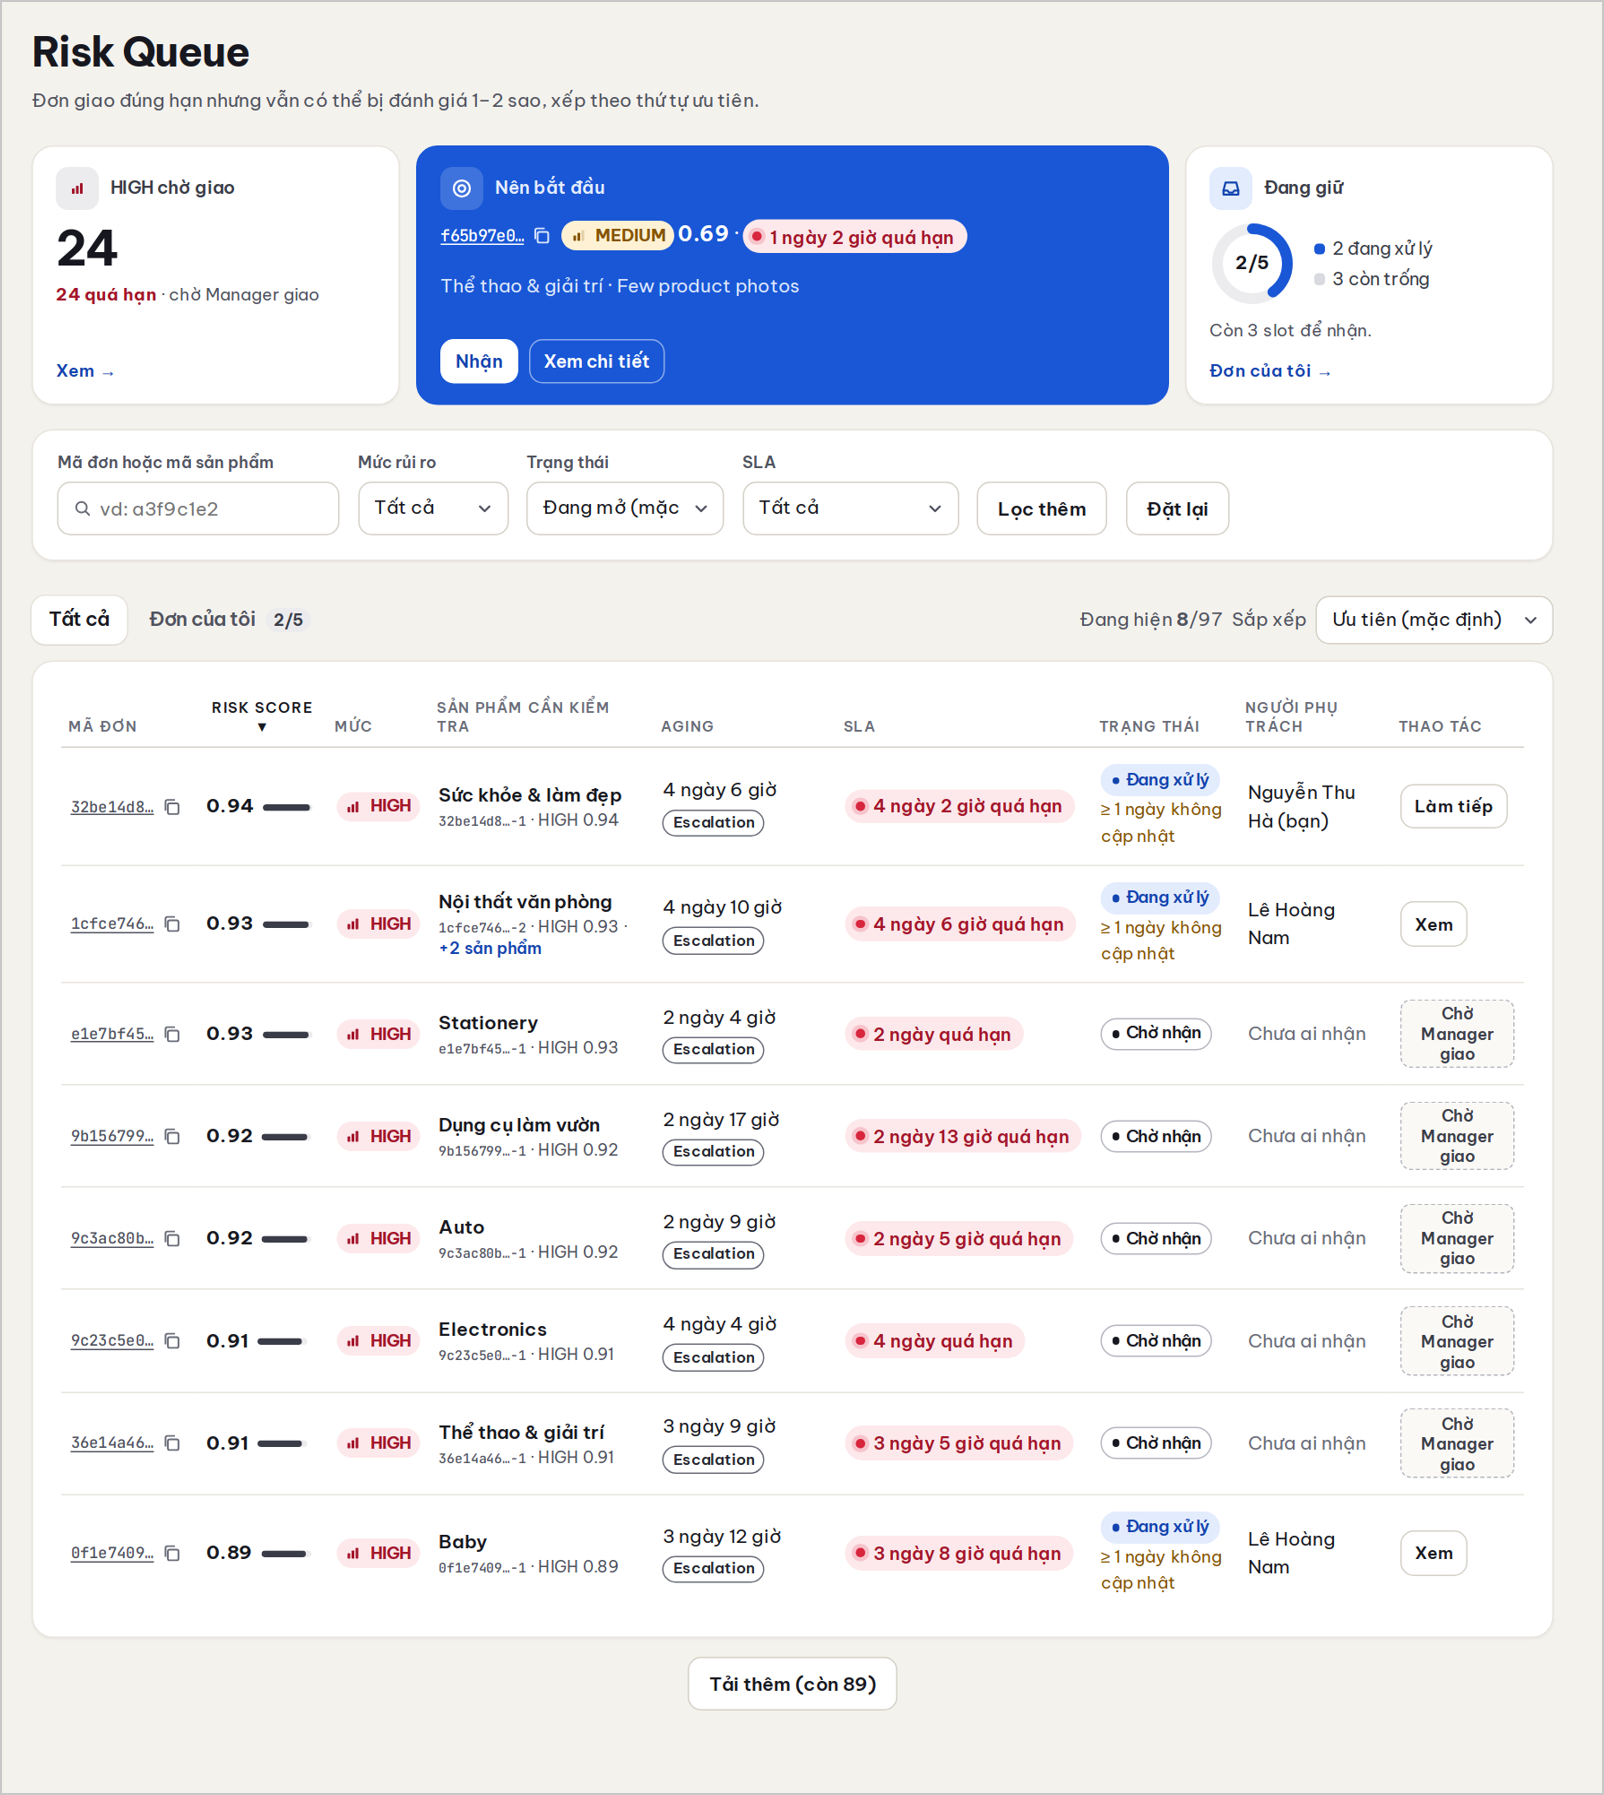
\includegraphics[width=\linewidth]{ui-risk-queue}
  \caption{Hàng đợi rủi ro của nhân viên: đơn sắp theo điểm, kèm sản phẩm có điểm cao nhất của mỗi đơn (dữ liệu demo).}\label{fig:ui-queue}
\end{figure}

% ---------------------------------------------------------------------
\subsection{Diễn giải điểm số ở mức đơn hàng}

Trang chi tiết đơn (Hình~\ref{fig:ui-detail}) là nơi người dùng đọc điểm số kỹ nhất, nên cũng là nơi dễ diễn giải sai nhất. Khối ``Kết quả model của đơn'' hiển thị bốn thông tin đi cùng điểm số: thanh điểm có vạch ngưỡng của mức trung bình và mức cao, luật tổng hợp, phiên bản mô hình và thời điểm dự báo, phiên bản ngưỡng. Bốn thông tin này giúp mọi con số trên màn hình truy ngược được về đúng lần chấm điểm đã sinh ra nó, cùng nguyên tắc với việc lưu cấu hình và mã commit của từng lần huấn luyện ở mục~\ref{sec:data}.

Ngay dưới điểm số là một câu nhắc cố định: điểm rủi ro dùng để ưu tiên kiểm tra, không phải kết luận khách không hài lòng. Câu nhắc này đến từ hai giới hạn đã nêu ở Chương~\ref{ch:method}. Thứ nhất, nhãn yếu ở mức item: điểm của sản phẩm là rủi ro đơn bị đánh giá thấp \emph{khi có mặt} sản phẩm đó, không phải bằng chứng sản phẩm gây ra bất mãn. Thứ hai, chỉ số đánh giá đo khả năng xếp hạng, không đo xác suất đúng của từng đơn.

Bảng sản phẩm trong đơn cho thấy điểm của từng item, và khối ``Yếu tố liên quan tới score'' được dành cho giải thích ở mức item. Trong bản demo, một số item có danh sách yếu tố minh họa đi kèm điểm số (Hình~\ref{fig:ui-multi}), số còn lại hiển thị ``chưa có giải thích''. Các yếu tố này là nhãn minh họa của dữ liệu demo, không phải giá trị SHAP; khối này là chỗ dành sẵn cho bước giải thích mô hình khi được thực hiện (mục~\ref{sec:demo-limits}). Hai chi tiết thiết kế giữ cho phần giải thích không bị đọc sai: khi thiếu giải thích, giao diện nói rõ là chưa có thay vì để trống, để người dùng không hiểu nhầm là đơn không có yếu tố rủi ro nào; khi có giải thích, ngay bên dưới luôn có câu ``các yếu tố này đi kèm điểm cao, không chứng minh nguyên nhân'', nhất quán với cách diễn giải giá trị SHAP như cách mô hình sử dụng đặc trưng chứ không phải tác động nhân quả.

\begin{figure}[htbp]\centering
  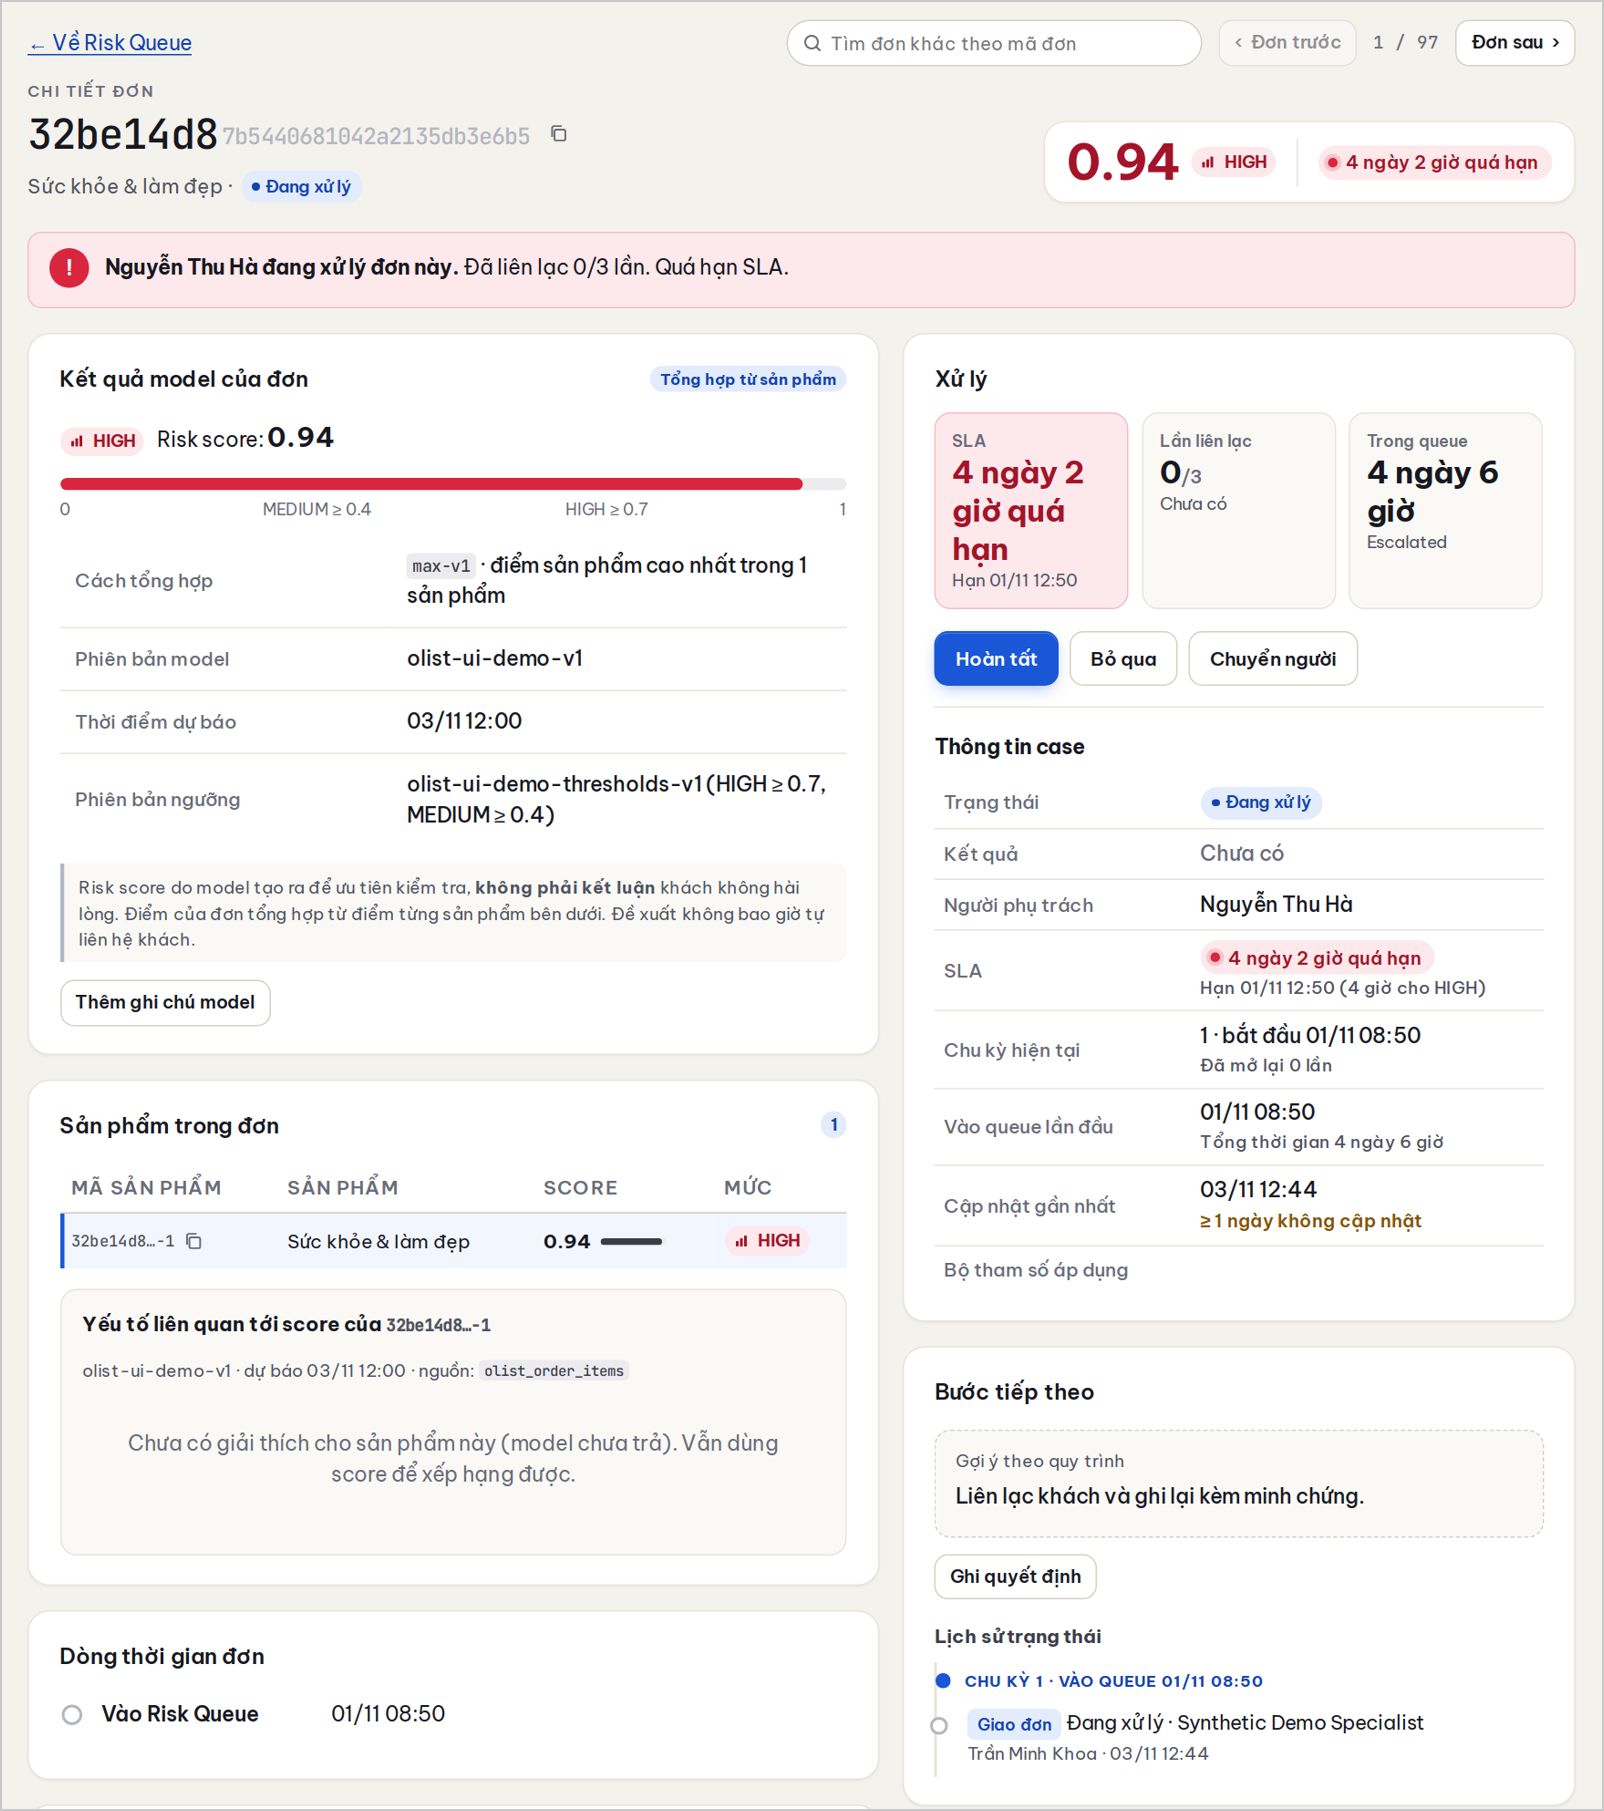
\includegraphics[width=\linewidth]{ui-order-detail}
  \caption{Chi tiết đơn: điểm số kèm vạch ngưỡng, luật tổng hợp, phiên bản mô hình và ngưỡng; điểm của từng sản phẩm (dữ liệu demo).}\label{fig:ui-detail}
\end{figure}

% ---------------------------------------------------------------------
\subsection{Theo dõi phân bố rủi ro}

Màn tổng quan của quản lý (Hình~\ref{fig:ui-dashboard}) tổng hợp số case theo mức rủi ro, theo ngày vào hàng đợi và theo khoảng điểm. Ngoài mục đích điều phối công việc, các khối này là công cụ quan sát đơn giản cho đầu ra của mô hình: nếu tỉ lệ đơn mức cao hoặc số case mới mỗi ngày thay đổi đột ngột giữa hai lần chấm điểm, quản lý thấy ngay mà không cần đọc báo cáo kỹ thuật. Như Bảng~\ref{tab:split} đã cho thấy, tỉ lệ dương dao động từ 10\% đến gần 14\% giữa các giai đoạn, nên việc theo dõi phân bố theo thời gian là cần thiết khi mô hình được dùng lâu dài.

Phần ``Xem theo khoảng score'' (Hình~\ref{fig:ui-bands}) chia các đơn theo năm khoảng điểm. Với dữ liệu demo, các khoảng gần như đều nhau: 15, 20, 26, 26 và 18 đơn từ khoảng thấp nhất tới cao nhất, tức điểm trung bình khoảng 0,52. Nếu đây là xác suất đã hiệu chỉnh, nó ngụ ý khoảng một nửa số đơn giao đúng hạn sẽ bị đánh giá thấp, trong khi tỉ lệ thực tế chỉ khoảng 10\%. Với một mô hình được hiệu chỉnh tốt, trung bình xác suất dự đoán phải xấp xỉ tỉ lệ dương, nên phần lớn đơn phải dồn về các khoảng điểm thấp. Vì vậy, bảng khoảng điểm là một phép kiểm tra nhanh mà quản lý tự làm được: nếu điểm trung bình lệch xa tỉ lệ đơn bị đánh giá thấp quan sát được, hoặc hình dạng phân bố thay đổi mạnh giữa hai lần chấm điểm, thì cần xem lại bước hiệu chỉnh hoặc dữ liệu đầu vào.

\begin{figure}[htbp]\centering
  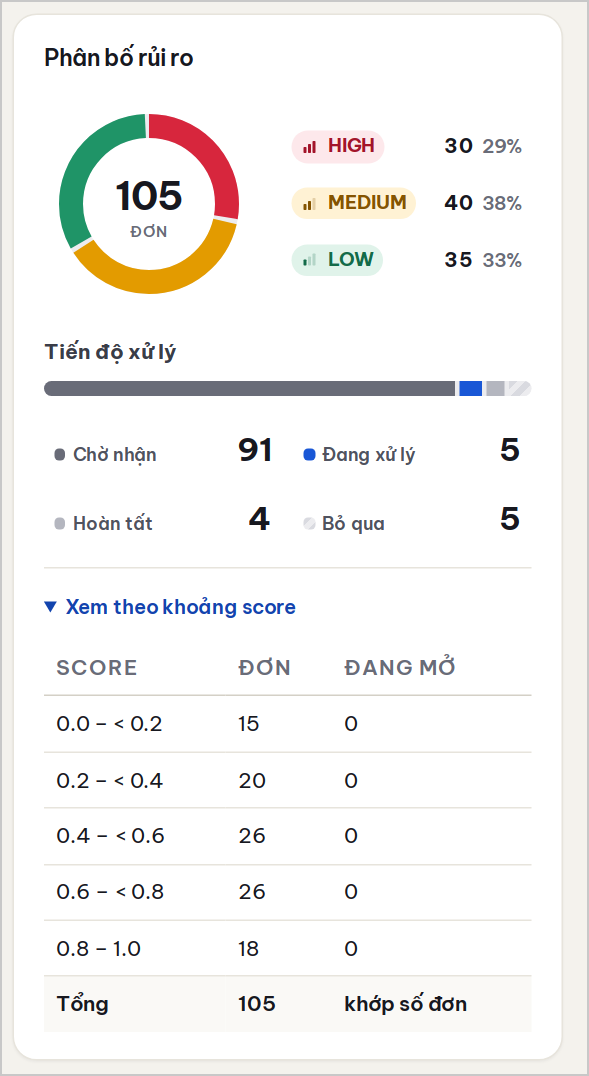
\includegraphics[width=0.45\linewidth]{ui-score-bands}
  \caption{Phân bố rủi ro và số đơn theo khoảng điểm (dữ liệu demo, điểm minh họa).}\label{fig:ui-bands}
\end{figure}

Chế độ ``Theo sản phẩm'' (Hình~\ref{fig:ui-product}) chuyển cùng các khối thống kê sang đơn vị item: 105 đơn trong bản demo gồm 114 sản phẩm, và danh sách sản phẩm có điểm cao nhất cho biết rủi ro tập trung ở danh mục nào. Hai chế độ tương ứng với hai đơn vị đã tách ở mục~\ref{sec:pipeline}: mô hình học và chấm điểm ở mức item, còn nhân viên xử lý ở mức đơn. Đặt hai góc nhìn cạnh nhau giúp người đọc không nhầm số sản phẩm rủi ro với số đơn cần liên hệ.

\begin{figure}[htbp]\centering
  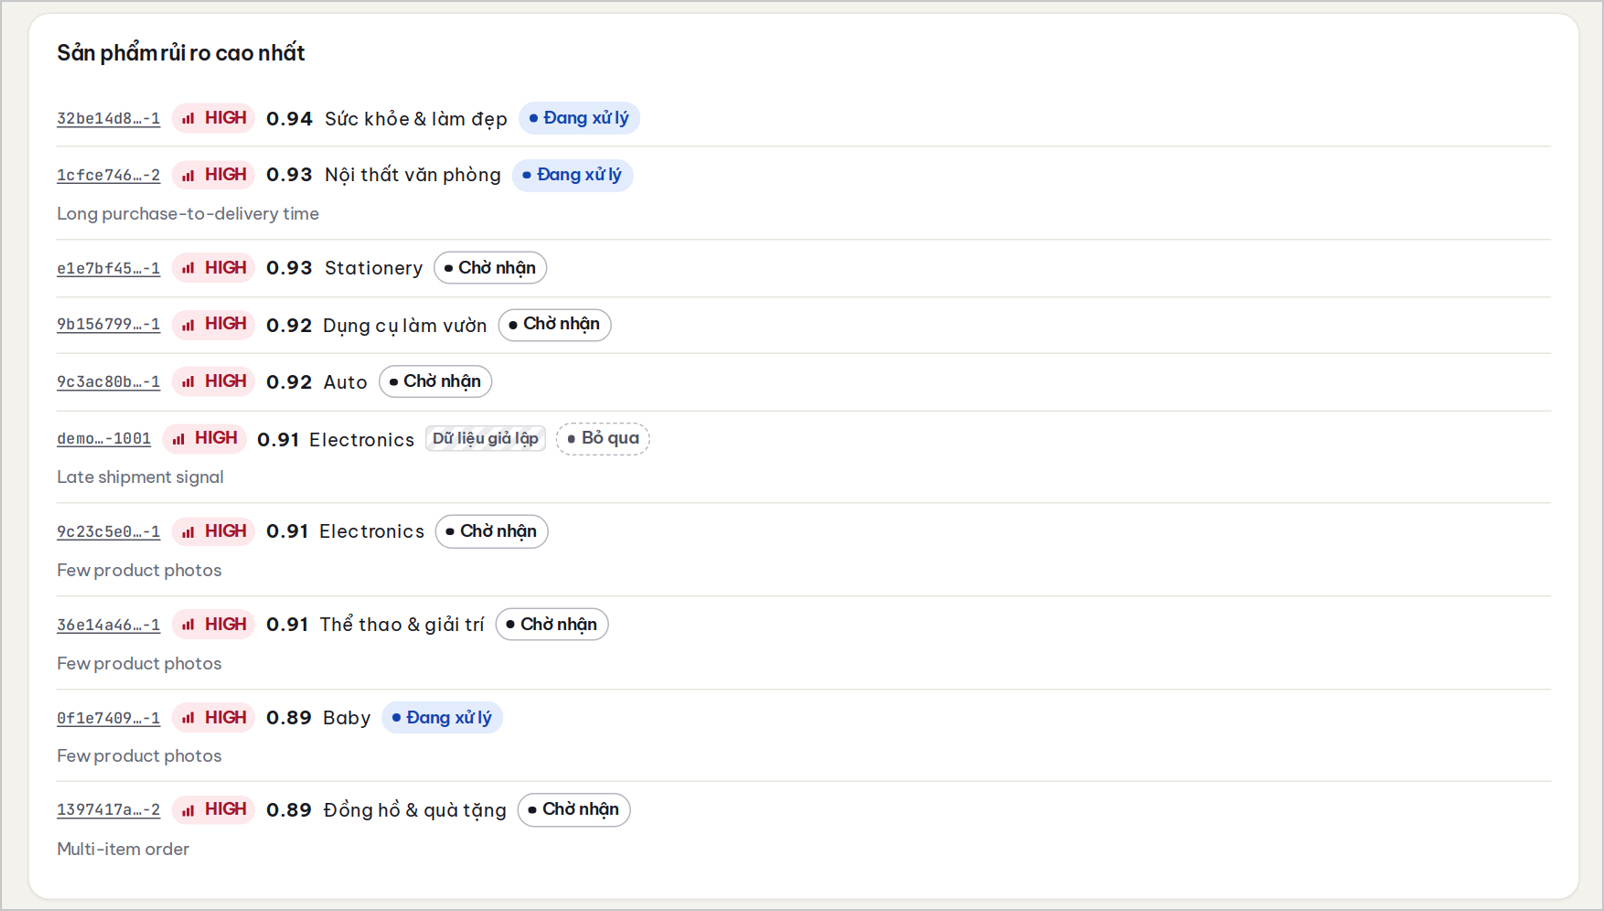
\includegraphics[width=\linewidth]{ui-product-view}
  \caption{Chế độ xem theo sản phẩm: các item có điểm cao nhất kèm danh mục và yếu tố minh họa (dữ liệu demo).}\label{fig:ui-product}
\end{figure}

Hình~\ref{fig:ui-dashboard} cũng minh họa trực quan giới hạn quan trọng nhất của bản demo: với ngưỡng cố định 0,7 và 0,4, mức HIGH chiếm 29\% số case, trong khi chính sách ở mục~\ref{sec:models} chỉ dành mức này cho 5\% đơn có điểm cao nhất. Điểm này được phân tích ở mục~\ref{sec:demo-limits} và Chương~5.

\begin{figure}[htbp]\centering
  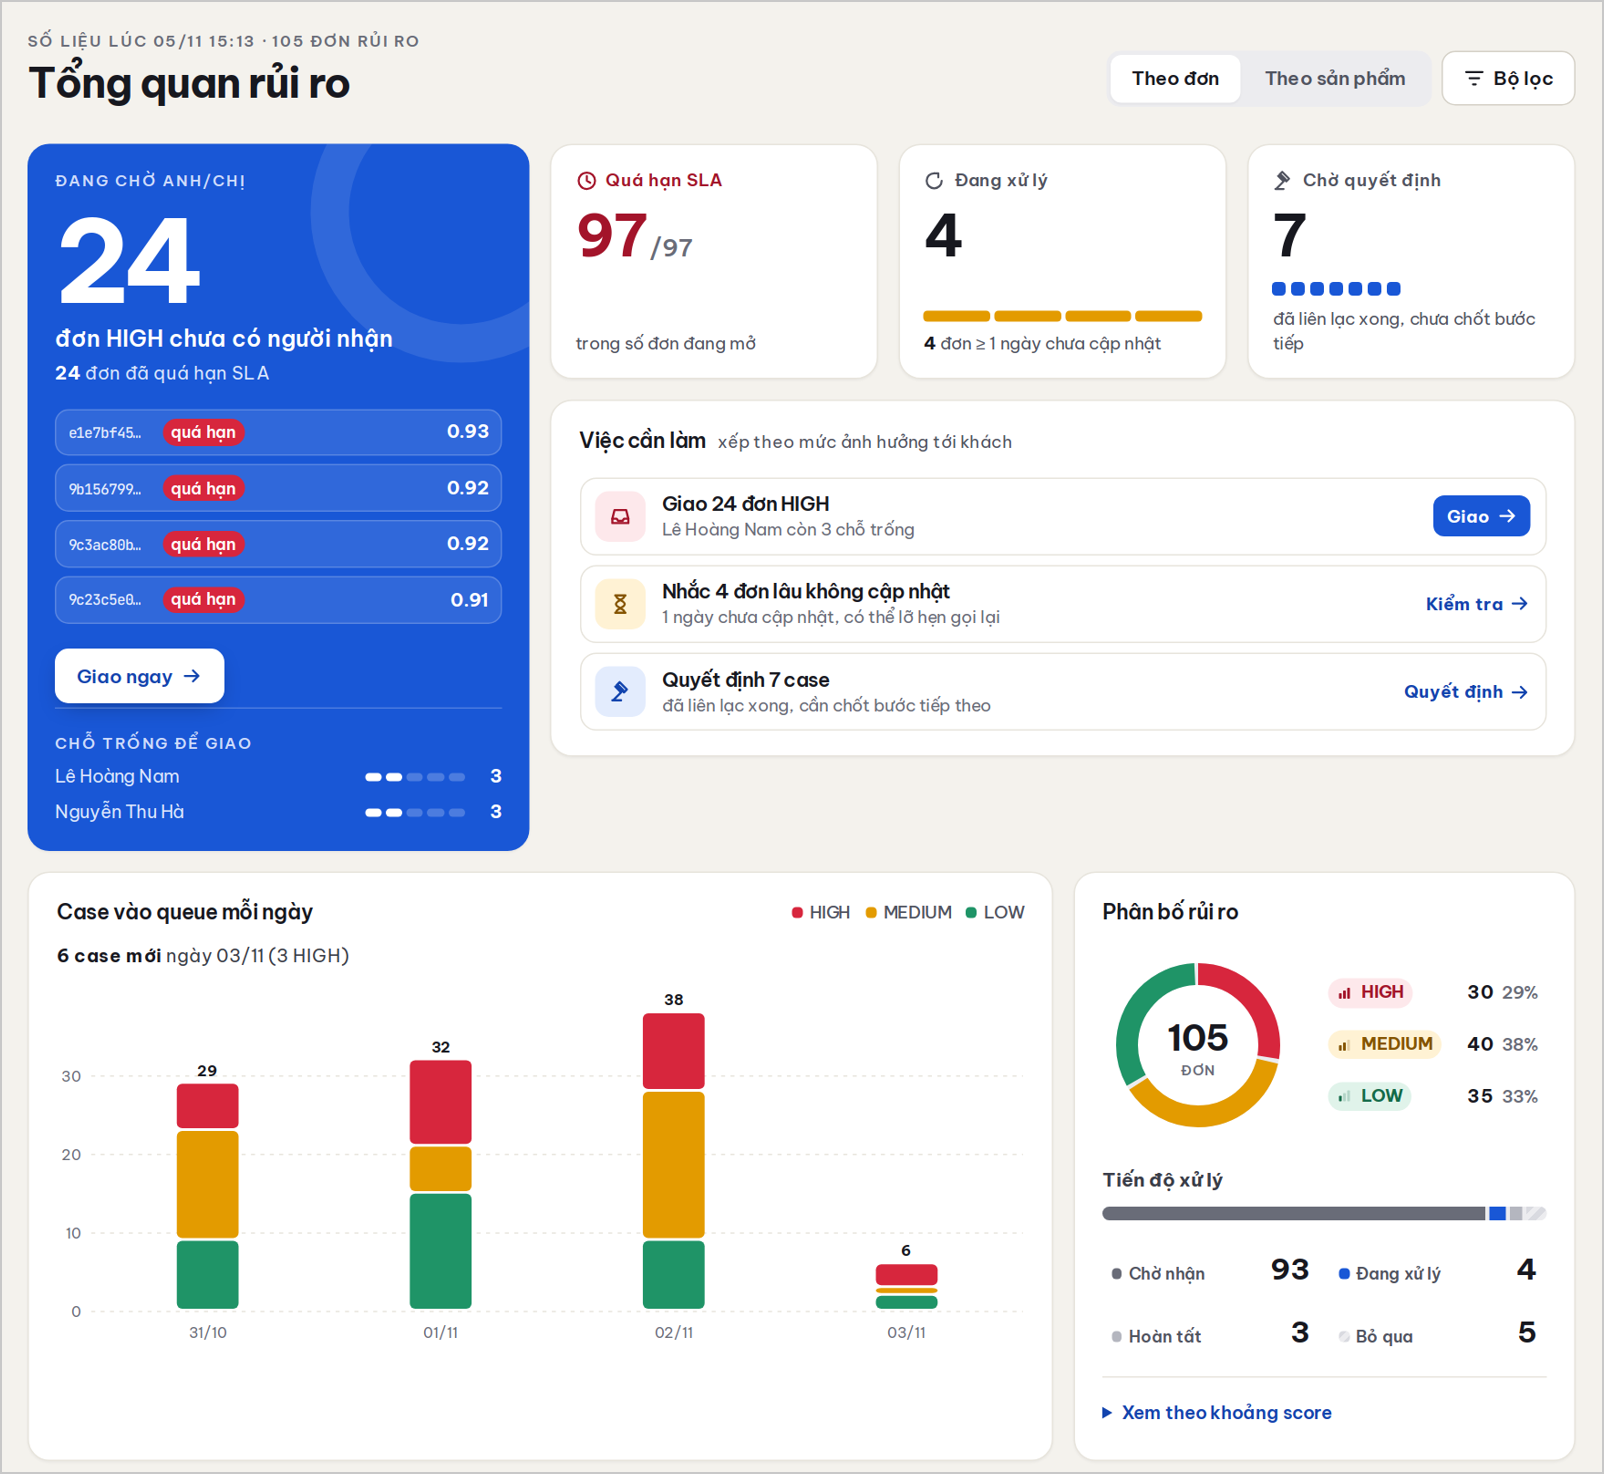
\includegraphics[width=\linewidth]{ui-dashboard}
  \caption{Tổng quan rủi ro của quản lý: case theo ngày và theo mức rủi ro (dữ liệu demo, ngưỡng cố định 0,7/0,4).}\label{fig:ui-dashboard}
\end{figure}

% ---------------------------------------------------------------------
\subsection{Dữ liệu vận hành phục vụ đánh giá mô hình}

Như đã nêu ở mục~\ref{sec:eval}, các chỉ số hiện tại chỉ đo khả năng dự báo, chưa đo hiệu quả can thiệp. Ứng dụng được thiết kế để tích lũy đúng loại dữ liệu cần cho bước đánh giá đó, theo ba nguyên tắc:

\begin{enumerate}
  \item \textbf{Điểm số chỉ đọc.} Không có thao tác nào sửa điểm hay mức rủi ro. Quản lý có thể thêm ghi chú về mô hình cho một đơn, nhưng ghi chú được lưu riêng. Nhờ vậy, sau này có thể so sánh điểm gốc với kết quả thực tế mà không lo điểm đã bị chỉnh tay.
  \item \textbf{Kết quả xử lý có cấu trúc.} Khi đóng case, nhân viên phải chọn một kết quả trong danh mục cố định (có vấn đề, không có vấn đề, trùng case) hoặc một lý do bỏ qua (không liên lạc được, khách từ chối, \ldots). Mỗi lần liên lạc được ghi lại với cách liên lạc và kết quả. Kết quả ``có vấn đề'' và ``không có vấn đề'' là một nguồn nhãn độc lập với đánh giá sao, có thể dùng để đo precision của nhóm HIGH trong vận hành thật.
  \item \textbf{Lịch sử chỉ thêm, không sửa.} Mọi thao tác đều được ghi lại với thời điểm và người thực hiện, nên có thể dựng lại đơn nào đã được liên hệ, khi nào, sau bao lâu kể từ lúc có điểm, để đối chiếu với nhãn quan sát được về sau.
\end{enumerate}

Mỗi lần liên hệ được ghi qua màn hình liên lạc khách (Hình~\ref{fig:ui-contact}) với thời điểm, phương thức, kết quả và ngày hẹn liên hệ tiếp. Đây là bản ghi \emph{can thiệp}, phần dữ liệu mà bộ Olist không có. Khi dùng để đánh giá, cần tách hai trường hợp dễ bị gộp chung: nếu sau số lần liên hệ tối đa vẫn không gặp được khách, case tự chuyển sang bỏ qua với lý do ``không liên lạc được'', nghĩa là can thiệp \emph{chưa xảy ra}; trường hợp này khác với can thiệp đã xảy ra nhưng khách vẫn đánh giá thấp. Gộp hai nhóm sẽ làm hiệu quả can thiệp trông thấp hơn thực tế.

\begin{figure}[htbp]\centering
  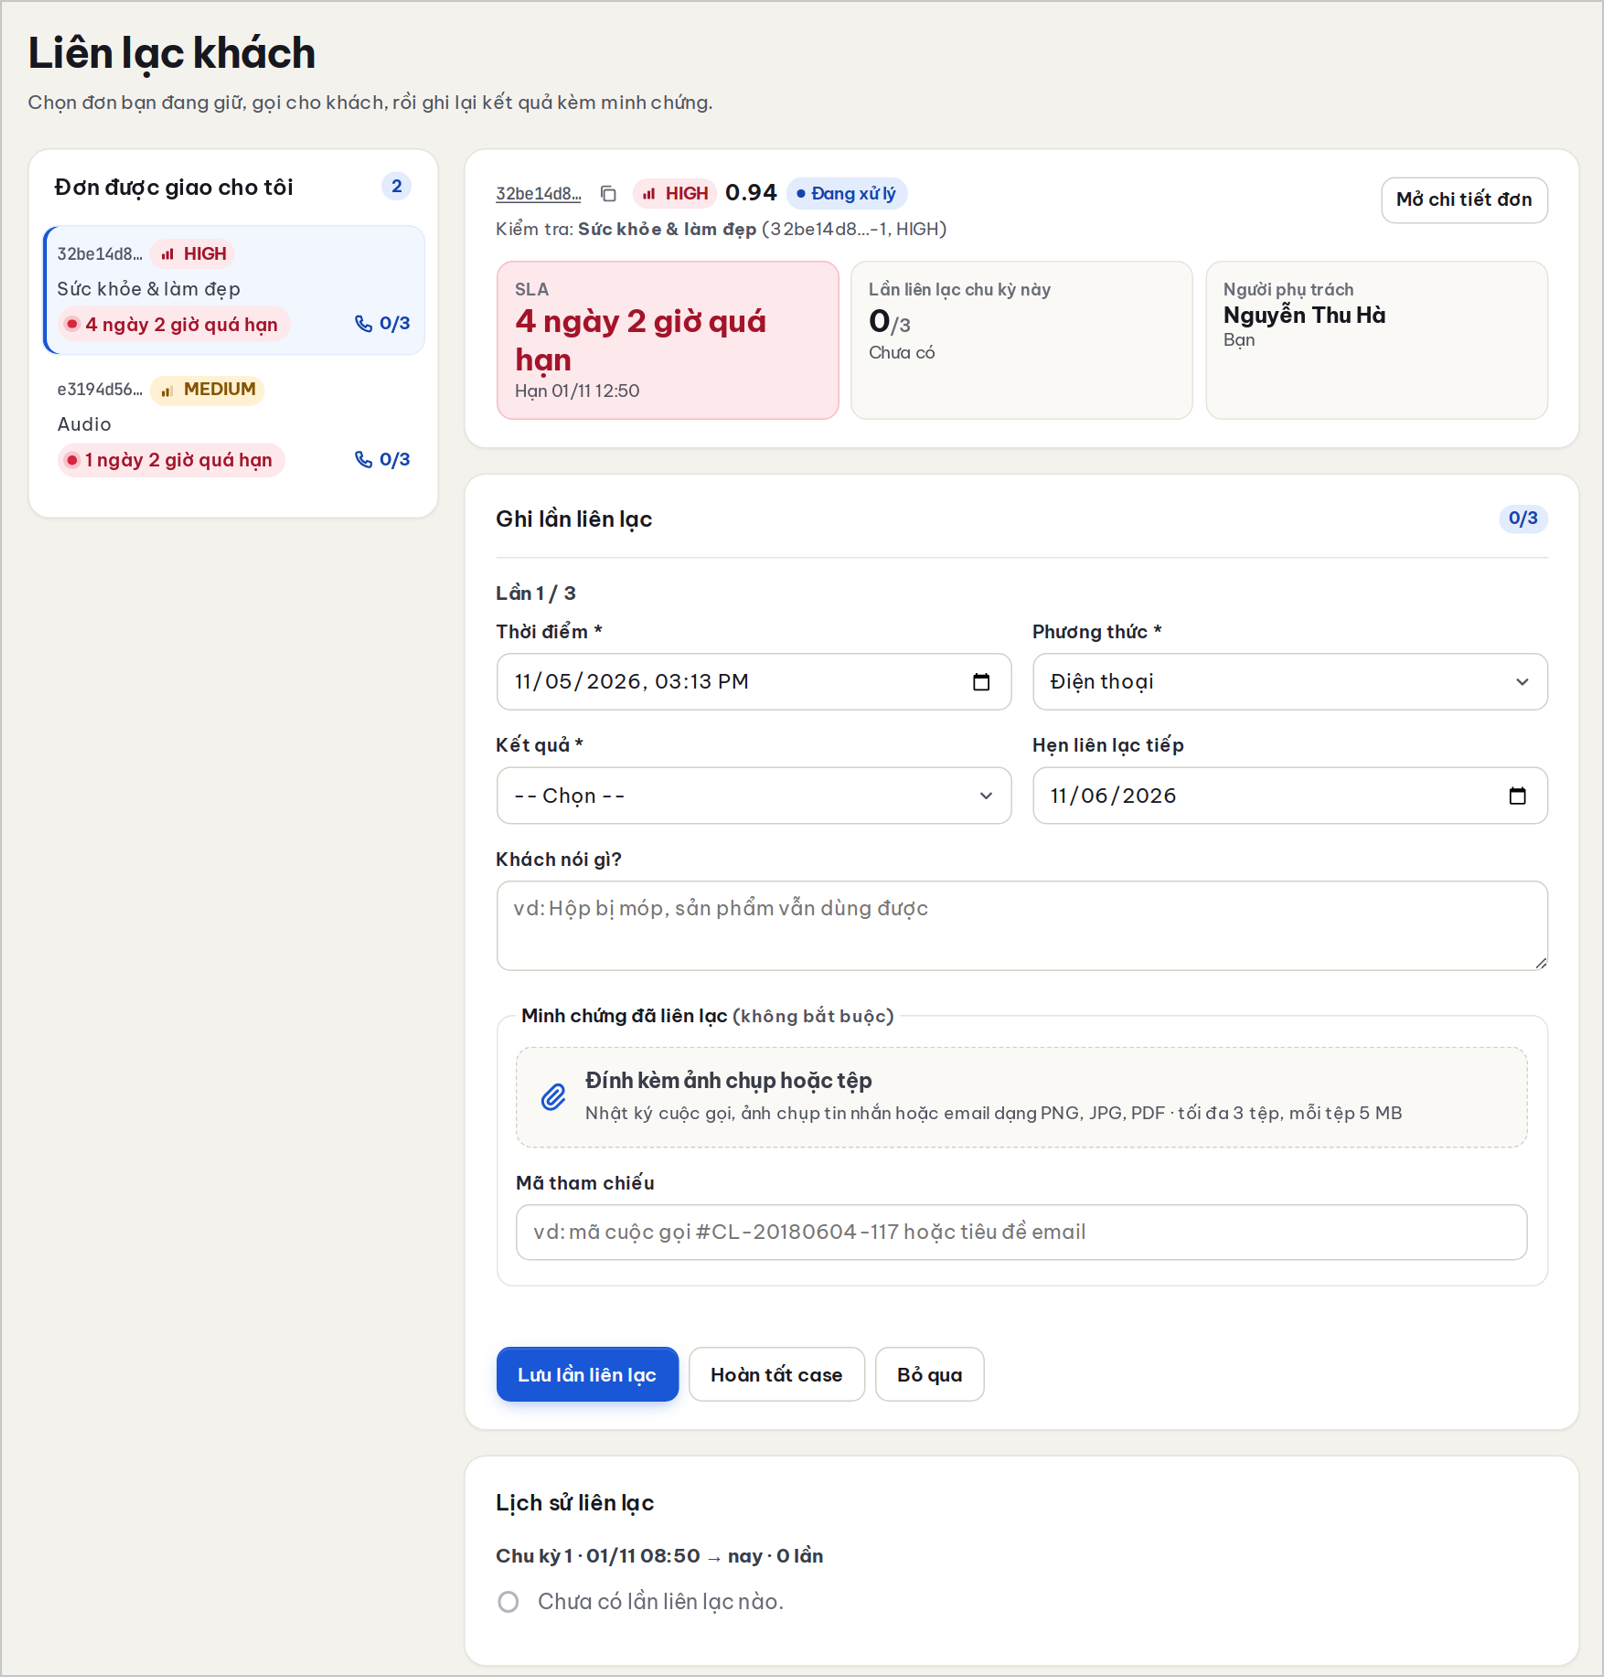
\includegraphics[width=\linewidth]{ui-contact-attempt}
  \caption{Màn hình liên lạc khách: mỗi lần liên hệ được ghi với thời điểm, phương thức, kết quả và minh chứng (dữ liệu demo).}\label{fig:ui-contact}
\end{figure}

Hình~\ref{fig:ui-closed} là một case đã đóng: điểm 0,68 ở mức trung bình nằm cạnh kết quả xử lý ``có vấn đề'', lần liên lạc và quyết định tiếp theo của quản lý. Mỗi case đóng như vậy là một cặp \emph{(điểm dự báo, kết quả quan sát)} gắn với đúng phiên bản mô hình đã sinh ra điểm. Hình~\ref{fig:feedback-loop} tóm tắt cách các cặp này quay lại phục vụ đánh giá và cải tiến mô hình.

\begin{figure}[htbp]\centering
  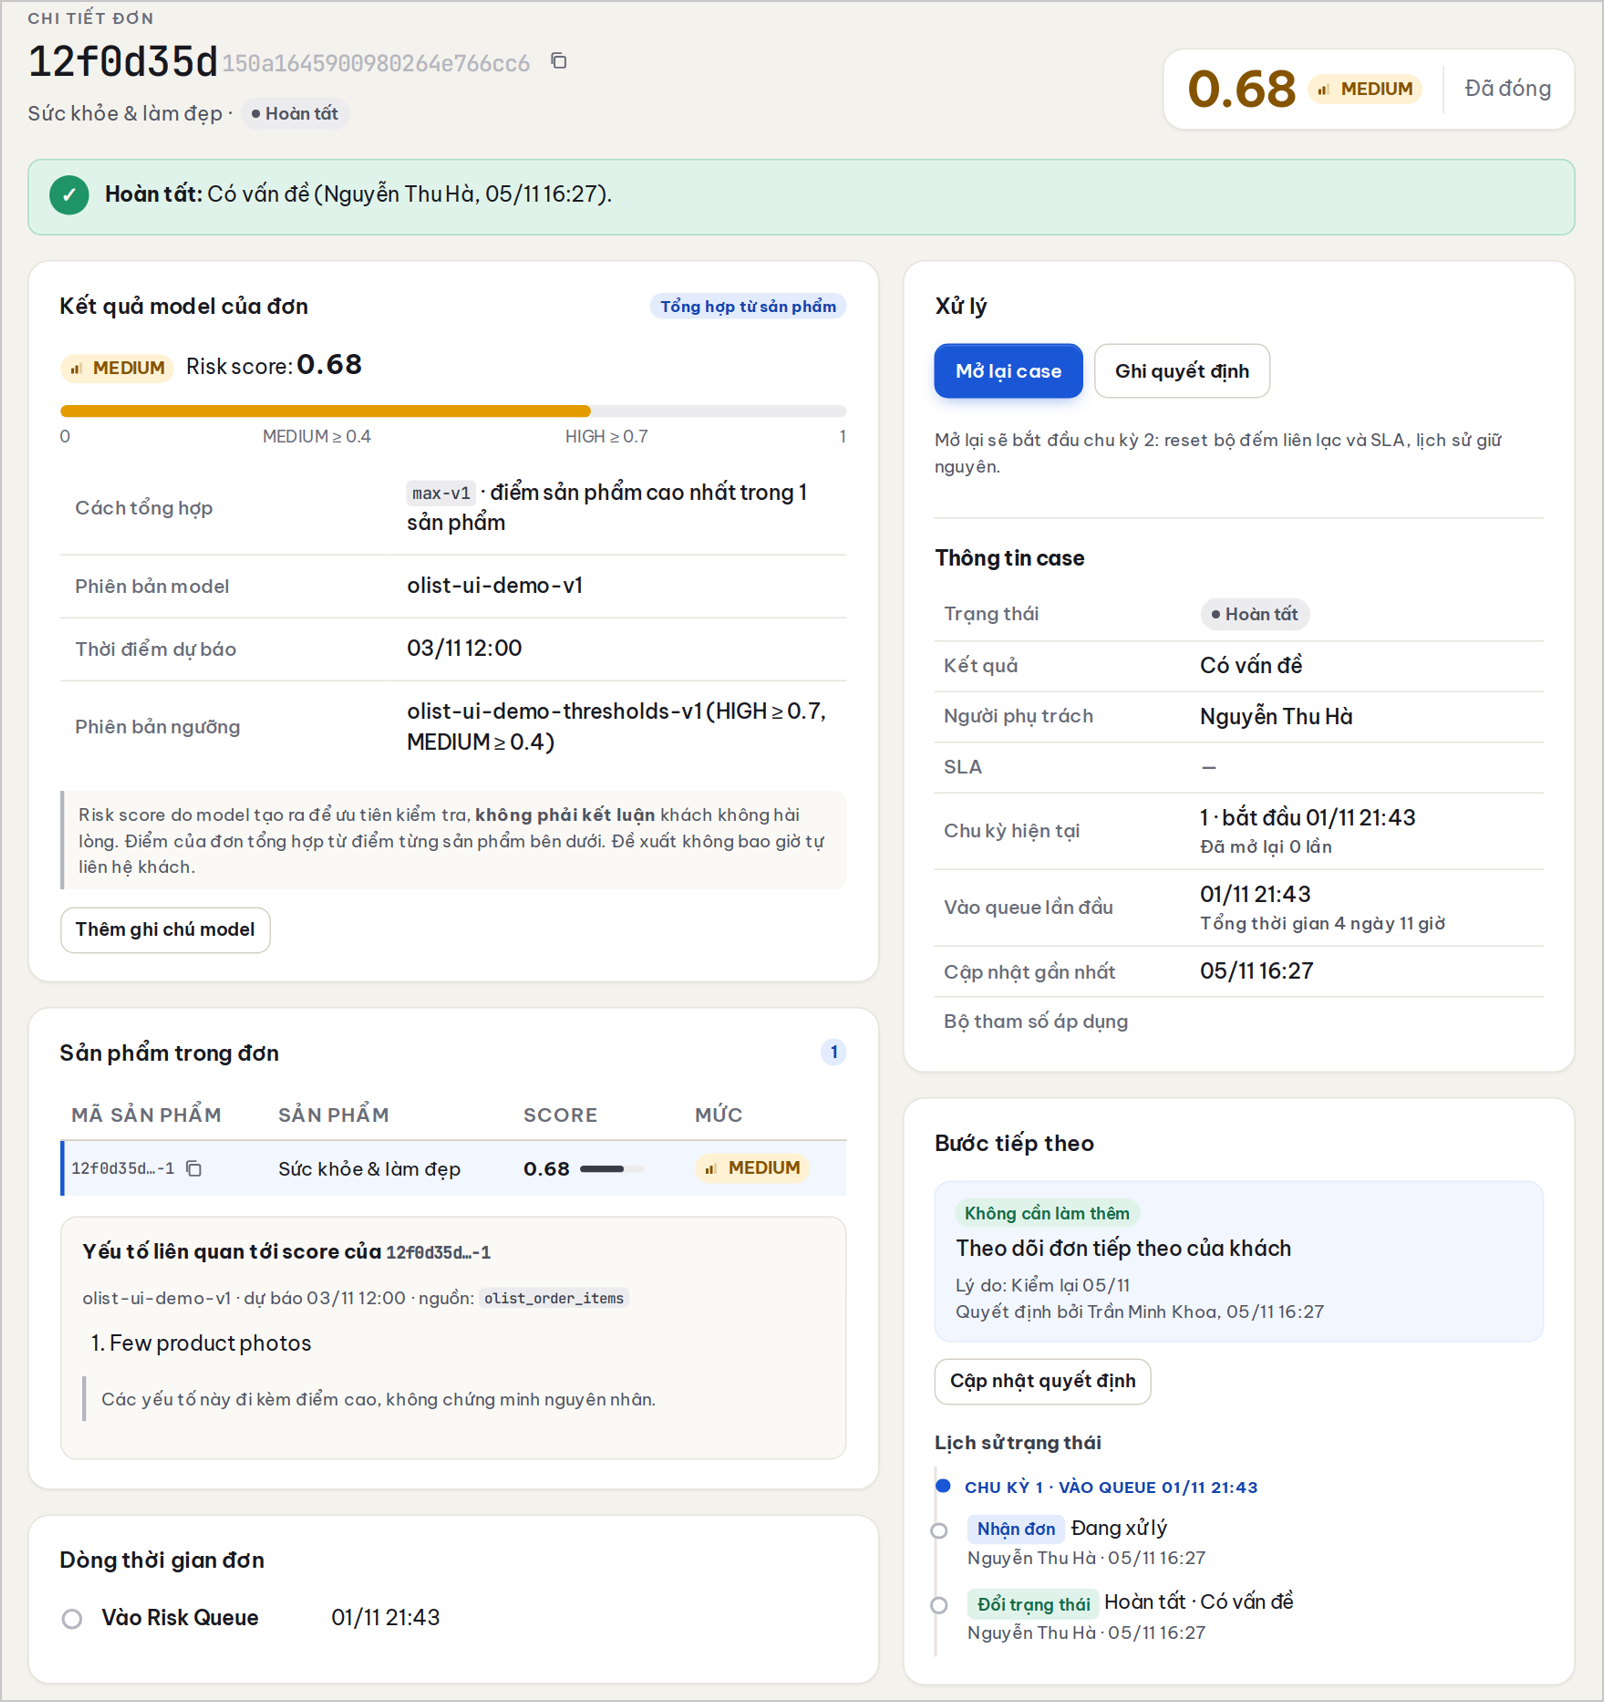
\includegraphics[width=\linewidth]{ui-closed-case}
  \caption{Case đã đóng: điểm dự báo, kết quả xử lý ``có vấn đề'' và lịch sử thao tác được lưu cùng nhau (dữ liệu demo).}\label{fig:ui-closed}
\end{figure}

\begin{figure}[htbp]\centering
\begin{tikzpicture}[font=\footnotesize, >={Latex}, node distance=0.55cm and 0.9cm,
  box/.style={draw,rounded corners,fill=#1,minimum width=3.4cm,minimum height=0.9cm,align=center}, box/.default=gray!10]
  \node[box=blue!15] (snap) {Snapshot dự đoán\\điểm, mức, phiên bản};
  \node[box=orange!20,right=of snap] (case) {Case trong\\hàng đợi ưu tiên};
  \node[box=teal!20,right=of case] (contact) {Liên hệ khách\\(các lần liên lạc)};
  \node[box=green!20,below=of contact] (outcome) {Kết quả xử lý\\có / không có vấn đề};
  \node[box=yellow!30,left=of outcome] (eval) {Cặp (điểm, kết quả)\\precision nhóm HIGH};
  \node[box=violet!20,left=of eval] (retrain) {Hiệu chỉnh, chọn ngưỡng\\hoặc huấn luyện lại};
  \node[box=red!15,below=of eval] (review) {Đánh giá sao của khách\\(nhãn $y$ ở Chương~3)};
  \draw[->] (snap) -- (case); \draw[->] (case) -- (contact); \draw[->] (contact) -- (outcome);
  \draw[->] (outcome) -- (eval); \draw[->] (review) -- (eval); \draw[->] (eval) -- (retrain);
  \draw[->,dashed] (retrain) -- node[right,font=\scriptsize]{phiên bản mới} (snap);
\end{tikzpicture}
\caption{Vòng phản hồi giữa ứng dụng và luồng học máy. Điểm số không bao giờ bị sửa; kết quả xử lý và đánh giá sao được đối chiếu với điểm gốc để đánh giá mô hình. Đường nét đứt là bước chưa được thực hiện trong đề tài.}\label{fig:feedback-loop}
\end{figure}

Ba nguyên tắc này biến ứng dụng thành điểm khởi đầu cho một thử nghiệm có đối chứng: nếu một phần đơn HIGH được chọn ngẫu nhiên để không liên hệ, dữ liệu sẵn có đủ để ước lượng tác động của việc liên hệ lên tỉ lệ đánh giá thấp, điều mà Chương~\ref{ch:method} xác định là nằm ngoài phạm vi đề tài.

% ---------------------------------------------------------------------
\subsection{Minh họa luật tổng hợp max-v1}\label{sec:demo-maxv1}

Luật max-v1 quyết định đơn nào lên đầu hàng đợi, nên cần thấy rõ nó khác cách lấy trung bình ở đâu. Bảng~\ref{tab:demo-maxv1} dùng ba đơn với điểm item \emph{giả định}, chỉ để minh họa cơ chế; mức rủi ro được gán theo ngưỡng của lần chạy rừng ngẫu nhiên đã nêu ở mục~\ref{sec:demo-limits} (mức cao từ 0,286, mức trung bình từ 0,112).

\begin{table}[htbp]\centering\small
\caption{Điểm đơn theo luật max-v1 và theo trung bình (điểm item giả định)}\label{tab:demo-maxv1}
\begin{tabular}{lp{3.4cm}cccc}
\toprule
Đơn & Điểm các item & max-v1 & Mức & Trung bình & Mức \\
\midrule
A & 0,08; 0,12; 0,41       & 0,41 & \textsc{Cao}        & 0,20 & \textsc{Trung bình} \\
B & 0,30                   & 0,30 & \textsc{Cao}        & 0,30 & \textsc{Cao} \\
C & 0,15; 0,16; 0,18; 0,20 & 0,20 & \textsc{Trung bình} & 0,17 & \textsc{Trung bình} \\
\bottomrule
\end{tabular}
\end{table}

Hình~\ref{fig:ui-multi} là một đơn ba sản phẩm trong bản demo: các item có điểm 0,93, 0,79 và 0,43, điểm của đơn là 0,93 theo max-v1, trong khi trung bình chỉ là 0,72. Giao diện đánh dấu item quyết định điểm của đơn ở dòng đầu bảng sản phẩm, nên người dùng thấy ngay điểm của đơn đến từ sản phẩm nào.

\begin{figure}[htbp]\centering
  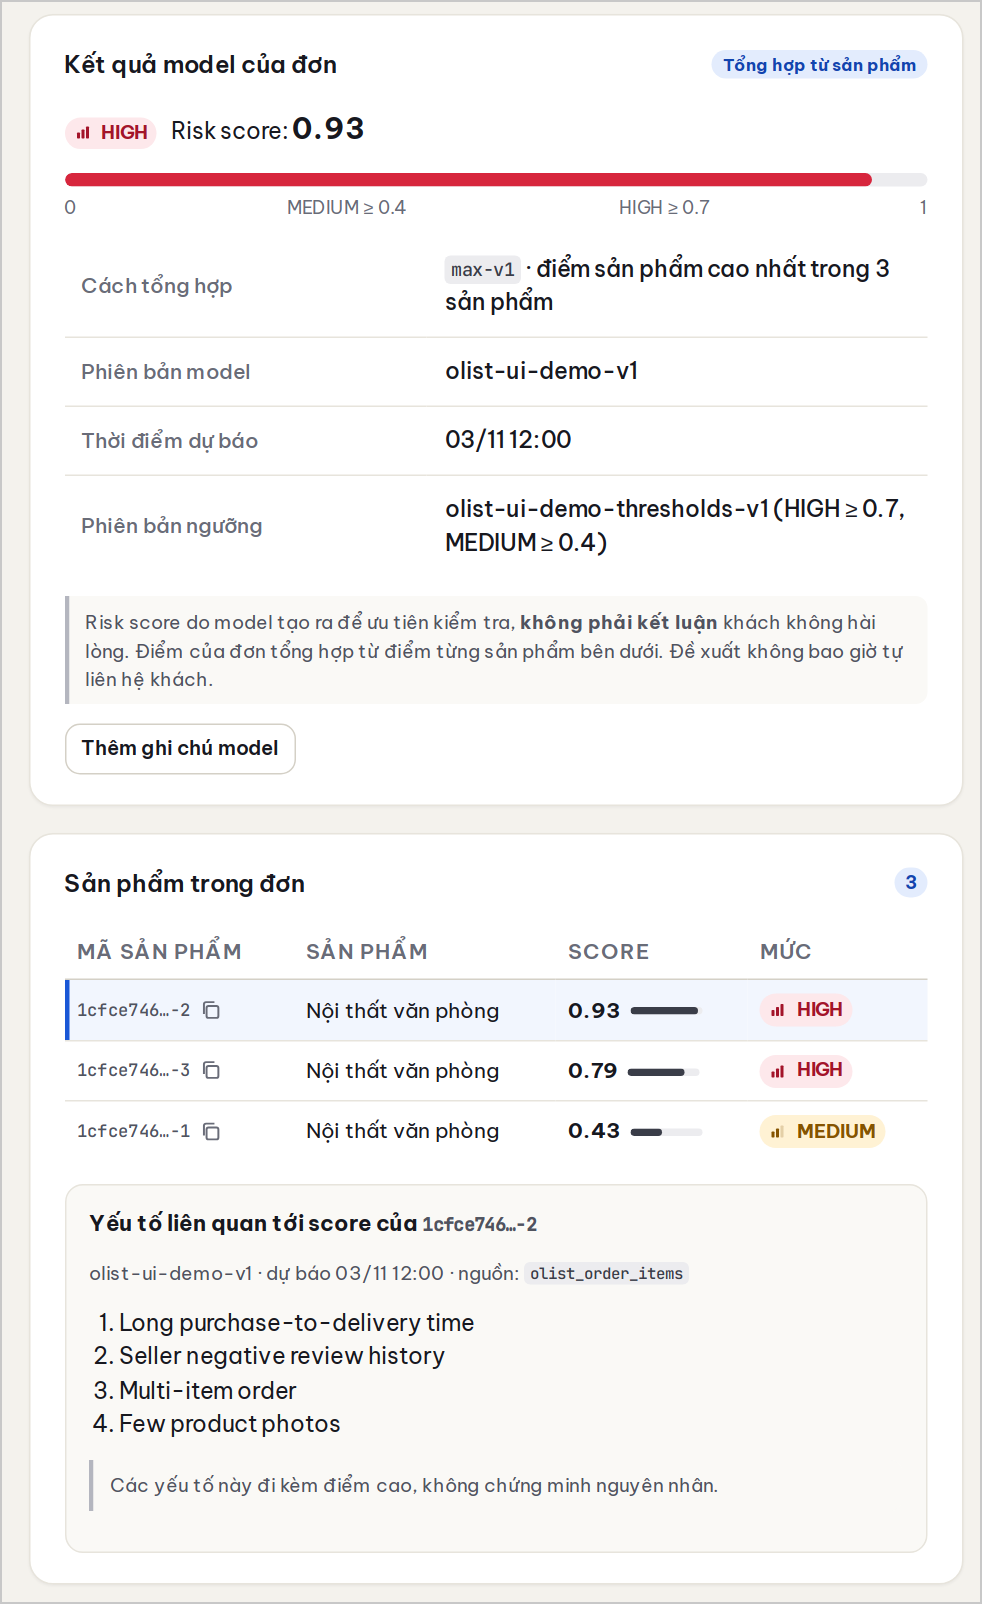
\includegraphics[width=0.62\linewidth]{ui-multi-item}
  \caption{Đơn ba sản phẩm: điểm của đơn (0,93) lấy từ item có điểm cao nhất; khối yếu tố đi kèm câu nhắc không chứng minh nguyên nhân (dữ liệu demo).}\label{fig:ui-multi}
\end{figure}

Theo max-v1, ba đơn giả định trong Bảng~\ref{tab:demo-maxv1} có thứ tự ưu tiên là A, B, C; theo trung bình, thứ tự là B, A, C. Khác biệt nằm ở đơn A: một sản phẩm có điểm 0,41 bị hai sản phẩm bình thường kéo xuống còn 0,20 nếu lấy trung bình, và đơn rơi khỏi mức cao. Đây đúng là tình huống ``mắt xích yếu nhất'' mà max-v1 được thiết kế để bắt (mục~\ref{sec:pipeline}). Đơn C cho thấy mặt trái của luật: bốn sản phẩm đều ở mức vừa phải, nhưng điểm của đơn bằng điểm cao nhất trong bốn, nên đơn nhiều sản phẩm có xu hướng được đẩy lên chỉ vì có nhiều cơ hội hơn để một item có điểm cao. Trên giao diện, cột sản phẩm cần kiểm tra (Hình~\ref{fig:ui-queue}) giúp người dùng nhận ra trường hợp này: nếu điểm của đơn đến từ một item duy nhất nổi bật, đó là tình huống A; nếu các item đều sát nhau, đó là tình huống C.

% ---------------------------------------------------------------------
\subsection{Tác động của ngưỡng lên danh sách ưu tiên}\label{sec:demo-threshold}

Bảng~\ref{tab:demo-threshold} so sánh tỉ lệ các mức rủi ro trong bản demo (ngưỡng cố định 0,7 và 0,4, đếm trên 105 case ở Hình~\ref{fig:ui-dashboard}) với tỉ lệ mà chính sách ngưỡng ở mục~\ref{sec:models} tạo ra. Vì điểm của bản demo không phải đầu ra của mô hình, bảng không so sánh hai bộ điểm mà so sánh hai \emph{cách đặt ngưỡng}.

\begin{table}[htbp]\centering\small
\caption{Tỉ lệ các mức rủi ro: ngưỡng cố định của bản demo và chính sách theo phần trăm}\label{tab:demo-threshold}
\begin{tabular}{lcccc}
\toprule
Cách đặt ngưỡng & Ngưỡng cao / trung bình & \textsc{Cao} & \textsc{Trung bình} & \textsc{Thấp} \\
\midrule
Cố định (bản demo, 105 case)        & 0,7 / 0,4         & 29\% (30) & 38\% (40) & 33\% (35) \\
Theo phần trăm (chính sách)         & $\approx$0,286 / $\approx$0,112 & 5\%  & 15\% & 80\% \\
\bottomrule
\end{tabular}
\end{table}

Ngưỡng theo phần trăm chỉ có nghĩa khi gắn với một con số năng lực cụ thể. Trong ứng dụng, con số đó là tham số vận hành do quản lý cài đặt (Hình~\ref{fig:ui-settings}): mỗi nhân viên giữ tối đa 5 đơn đang xử lý và liên hệ tối đa 3 lần mỗi chu kỳ. Với hai nhân viên trong bản demo, hệ thống xử lý cùng lúc khoảng 10 đơn, trong khi hàng đợi có 30 đơn mức cao và 40 đơn mức trung bình. Giống như mô hình và ngưỡng, mỗi thay đổi tham số tạo một phiên bản mới có thời điểm hiệu lực và lý do, nên có thể biết một đơn được xử lý dưới năng lực nào khi đánh giá về sau.

\begin{figure}[htbp]\centering
  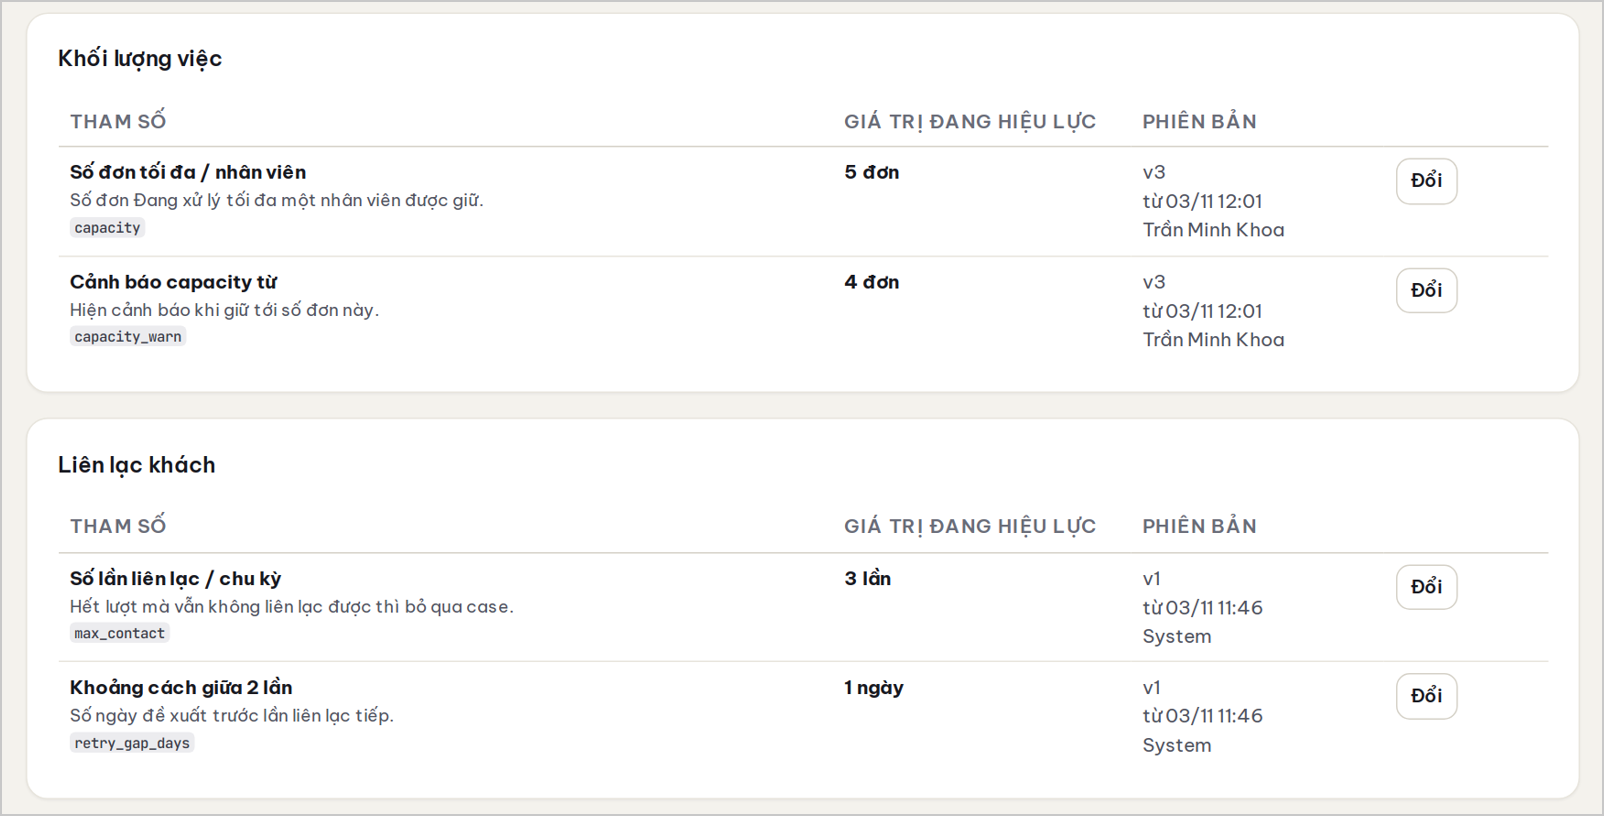
\includegraphics[width=\linewidth]{ui-settings-capacity}
  \caption{Tham số năng lực xử lý: số đơn tối đa mỗi nhân viên và số lần liên lạc mỗi chu kỳ, kèm phiên bản và thời điểm hiệu lực (dữ liệu demo).}\label{fig:ui-settings}
\end{figure}

Hai cách đặt ngưỡng cho ra hai hàng đợi rất khác nhau. Với ngưỡng cố định, gần một phần ba số đơn ở mức cao, nghĩa là quản lý phải tự phân công khoảng 30 đơn mỗi đợt thay vì khoảng 5 đơn; khi mọi thứ đều ``cao'', mức cao không còn giúp chọn ra đơn cần làm trước. Ngưỡng theo phần trăm giữ cho số đơn mức cao bằng đúng năng lực xử lý, bất kể điểm số tuyệt đối của mô hình cao hay thấp. Chiều ngược lại cũng sai: ngưỡng mức cao ghi nhận được với rừng ngẫu nhiên chỉ khoảng 0,286, nên nếu giữ ngưỡng cố định 0,7 khi thay bằng điểm thật, số đơn mức cao sẽ ít hơn nhiều so với 5\% và phần năng lực dành cho nhóm này bị bỏ trống.

% ---------------------------------------------------------------------
\subsection{Giới hạn của bản demo}\label{sec:demo-limits}

Bản demo chứng minh luồng từ điểm số đến hành động chạy được từ đầu đến cuối, nhưng chưa chứng minh mô hình mang lại giá trị trong vận hành. Có ba khoảng cách giữa bản demo và kết quả nghiên cứu:

\begin{enumerate}
  \item \textbf{Điểm số minh họa thay vì điểm của mô hình.} Mô hình rừng ngẫu nhiên được giữ lại chưa được đóng gói và đưa vào ứng dụng. Lần rà soát toàn luồng ngày 31/10/2026 ghi nhận tệp mô hình nạp được và dự đoán được khi gọi trực tiếp, nhưng không đọc được qua bộ chuyển đổi của ứng dụng vì khác định dạng đóng gói. Ngoài ra, chấm điểm chính thức trên giai đoạn kiểm tra cần chờ một tập kiểm tra chưa từng được xem, như đã nêu ở mục~\ref{sec:eval}.
  \item \textbf{Ngưỡng cố định thay vì ngưỡng theo năng lực.} Bản demo dùng ngưỡng 0,7 và 0,4. Với mô hình thật, ngưỡng được chọn theo tỉ lệ phần trăm trên phân vùng chọn ngưỡng; lần chạy rừng ngẫu nhiên trước đó ghi nhận ngưỡng mức cao khoảng 0,286 và mức trung bình khoảng 0,112 (mục~\ref{sec:demo-threshold}).
  \item \textbf{Chưa có giải thích mô hình.} Khối yếu tố rủi ro trên giao diện đã có chỗ, nhưng chưa có lần tính SHAP nào được lưu, nên nhân viên chỉ thấy điểm mà chưa thấy lý do.
\end{enumerate}

Nhờ ứng dụng chỉ đọc bảng dự đoán, cả ba khoảng cách này đều được xử lý ở phía luồng học máy: chấm điểm bằng mô hình thật, ghi ngưỡng tương ứng vào bảng ngưỡng và bổ sung yếu tố rủi ro vào snapshot mới. Giao diện và quy trình xử lý không cần thay đổi.
  % phần giao diện/demo (Trúc)

% Chương 5 — Thảo luận (Trúc). Nguồn số liệu: SERVER_CONTEXT/chapter4_evidence.md, model_variant_fold_metrics.md,
% TODO: đối chiếu mọi số metric với bảng Huy gửi cho Ch.4 trước khi nộp.
% reports/P5-accuracy-coursework-summary.md, P5-accuracy-failure-analysis.md (nhánh dev); mục "Giới hạn diễn giải"
% chuyển từ _moved_from_ch3.tex. Chỉ dùng số đã có trong evidence; không suy thêm chỉ số chưa được tính.
\chapter{Thảo luận}\label{ch:discussion}

Chương này đặt các kết quả của Chương~4 trở lại câu hỏi nghiên cứu ở Chương~\ref{ch:method}: chỉ với thông tin có tại thời điểm giao hàng, mô hình ước lượng rủi ro đánh giá thấp tốt đến đâu, và danh sách ưu tiên có giúp bộ phận chăm sóc khách hàng tiếp cận đúng khách hơn chọn ngẫu nhiên hay không. Mục~\ref{sec:disc-goals} so sánh kết quả với mục tiêu; mục~\ref{sec:disc-sw} trình bày điểm mạnh và hạn chế; mục~\ref{sec:disc-findings} nêu các phát hiện đáng chú ý. Mọi số liệu trong chương là kết quả trên các fold phát triển và mang tính thăm dò.

% =====================================================================
\section{So sánh với mục tiêu ban đầu}\label{sec:disc-goals}

Bảng~\ref{tab:disc-goals} đối chiếu từng mục tiêu với kết quả đạt được. Mốc so sánh cho PR-AUC là tỉ lệ dương, vì đó là PR-AUC kỳ vọng của một cách xếp hạng ngẫu nhiên; tỉ lệ dương của phân vùng huấn luyện là 10,13\% (Bảng~\ref{tab:split}). Mốc so sánh cho Recall@5\% là 5\%, mức recall kỳ vọng khi chọn ngẫu nhiên 5\% số đơn.

\begin{table}[htbp]\centering\small
\caption{Đối chiếu kết quả với mục tiêu}\label{tab:disc-goals}
\begin{tabular}{>{\raggedright\arraybackslash}p{4.1cm}>{\raggedright\arraybackslash}p{4.6cm}>{\raggedright\arraybackslash}p{2.3cm}>{\raggedright\arraybackslash}p{2.6cm}}
\toprule
Mục tiêu & Kết quả & Mốc so sánh & Đánh giá \\
\midrule
Xếp hạng tốt hơn ngẫu nhiên ở mức đơn & PR-AUC mức đơn trung bình 0,1465 (ba fold: 0,1425--0,1507) & khoảng 0,10 & Đạt, mức vượt khiêm tốn \\
Tìm đúng đơn khi chỉ xử lý được 5\% & Recall@5\% trung bình 0,1212 & 0,05 & Đạt, gấp khoảng 2,4 lần \\
Mục tiêu dừng của kế hoạch cải thiện & PR-AUC lăn 0,1465 & 0,25 & Chưa đạt \\
Cải thiện so với mô hình ban đầu & PR-AUC lăn tăng từ 0,1363 lên 0,1465 & mô hình ban đầu & Đạt (+7,5\%) \\
Ước lượng cuối cùng trên tập kiểm tra niêm phong & Chưa thực hiện & -- & Chưa đạt \\
Hệ thống xử lý case dựa trên điểm số & Chạy đủ luồng từ điểm số đến xử lý case & -- & Đạt, dùng điểm minh họa \\
\bottomrule
\end{tabular}
\end{table}

Kết quả trả lời câu hỏi nghiên cứu theo hai chiều. Về khả năng xếp hạng, câu trả lời là \emph{có, nhưng ở mức hạn chế}: PR-AUC cao hơn mốc ngẫu nhiên khoảng 45\%, và mức vượt này ổn định qua cả ba fold chứ không chỉ xuất hiện ở một giai đoạn. Về giá trị vận hành, Recall@5\% bằng 0,1212 nghĩa là nếu bộ phận chăm sóc khách hàng chỉ liên hệ được 5\% số đơn giao đúng hạn, danh sách theo mô hình chứa khoảng 12\% số đơn sẽ bị đánh giá thấp, gấp khoảng 2,4 lần so với chọn ngẫu nhiên. Nói cách khác, cùng một ngân sách liên hệ, mô hình giúp tiếp cận số khách có nguy cơ nhiều gấp đôi; nhưng gần 88\% khách sẽ đánh giá thấp vẫn nằm ngoài danh sách.

Mục tiêu PR-AUC 0,25 không đạt. Kế hoạch cải thiện đã thử mười giai đoạn có kiểm soát, giữ lại ba nhóm đặc trưng và dừng có chủ đích khi các thử nghiệm tiếp theo không còn cải thiện ổn định. Việc dừng ở đây là một kết quả, không phải một thiếu sót về nỗ lực: khi mô hình phức tạp hơn và đặc trưng phong phú hơn đều không vượt được mô hình đã chọn, khả năng cao là giới hạn nằm ở lượng tín hiệu có trong dữ liệu tại thời điểm giao hàng chứ không nằm ở thuật toán (mục~\ref{sec:disc-findings}).

% =====================================================================
\section{Điểm mạnh và hạn chế}\label{sec:disc-sw}

\subsection{Điểm mạnh}

\textbf{Đánh giá trong đúng điều kiện sử dụng.} Ba quyết định thiết kế làm cho con số khiêm tốn ở trên đáng tin hơn những con số cao hơn thường gặp: chia dữ liệu theo thời gian thay vì ngẫu nhiên, đặc trưng lịch sử chỉ dùng các đơn đã giao \emph{và} đã được đánh giá trước thời điểm dự đoán, và mỗi phân vùng dữ liệu chỉ phục vụ một quyết định. Các nghiên cứu chia ngẫu nhiên trên cùng bộ dữ liệu cho phép mô hình học từ tương lai~\cite{orman2026}, nên kết quả của họ và của đề tài không so sánh trực tiếp được; điều đề tài đo được là hiệu năng khi mô hình thực sự được dùng sau khi đơn vừa giao.

\textbf{Mỗi lựa chọn đều có mốc đối chứng.} Mô hình được chọn bằng trung bình ba fold rolling-origin thay vì một tập kiểm định, mỗi nhóm đặc trưng chỉ được giữ khi cải thiện chỉ số chính, và việc bỏ từng nhóm (leave-one-group-out) xác nhận cả ba nhóm được giữ đều cần thiết. Nhờ vậy, mỗi thành phần trong mô hình cuối cùng đều có bằng chứng riêng cho sự có mặt của nó.

\textbf{Kết nối được với vận hành.} Ngưỡng theo phần trăm biến năng lực xử lý thành tham số của mô hình; luật max-v1 được đánh số phiên bản; điểm số được ghi kèm phiên bản mô hình và ngưỡng; ứng dụng không cho phép sửa điểm và ghi lại kết quả xử lý có cấu trúc (mục~\ref{sec:demo}). Đây là nền tảng cần thiết để đánh giá hiệu quả can thiệp ở giai đoạn sau, điều mà phần lớn nghiên cứu dự báo sự hài lòng chưa đặt ra.

\subsection{Hạn chế}

\textbf{Kết quả chưa phải ước lượng cuối cùng.} Giai đoạn kiểm tra lịch sử đã bị lộ trong quá trình phát triển, nên mọi kết quả trên giai đoạn này được xếp loại thăm dò. Kết luận xác nhận cần một tập kiểm tra mới, được khóa trước khi xem. Cùng với đó, khoảng tin cậy bootstrap theo cụm đơn hàng, đường cong precision--recall và đường cong hiệu chỉnh trên tập kiểm tra chưa được tính.

\textbf{So sánh chưa đầy đủ.} Kho lưu trữ chỉ giữ số liệu theo fold của rừng ngẫu nhiên và ba cấu hình CatBoost; số liệu của mô hình tỉ lệ nền, hồi quy logistic và HistGradientBoosting không còn, nên chưa có một bảng so sánh công bằng giữa năm họ mô hình trên cùng bộ đặc trưng. Đề tài cũng chưa so với chính sách xếp theo giá trị đơn, một mốc đơn giản mà nghiên cứu gần đây cho thấy đôi khi khó vượt qua~\cite{li2026valuesorting}.

\textbf{Nhãn yếu và tự chọn.} Mỗi item thừa hưởng nhãn của đơn, nên trong đơn nhiều sản phẩm, mô hình học cả những item không liên quan tới sự bất mãn. Nhãn chỉ có ở các đơn có đánh giá, mà việc viết đánh giá là một quá trình tự chọn~\cite{li2008}.

\textbf{Chưa có giải thích mô hình và chưa có điểm thật trong ứng dụng.} Chưa có lần tính SHAP nào, nên chưa biết mô hình dựa vào đặc trưng nào cho từng đơn. Ứng dụng đang chạy với điểm minh họa và ngưỡng cố định (mục~\ref{sec:demo-limits}).

\subsection{Giới hạn khi diễn giải kết quả}

Kết quả của đề tài cần được hiểu trong các giới hạn sau:
\begin{itemize}
  \item Không có đánh giá không có nghĩa là khách hài lòng, do quá trình tự chọn khi viết đánh giá~\cite{li2008}.
  \item Đánh giá thấp không đồng nghĩa với việc khách rời bỏ hoặc gây thiệt hại doanh thu.
  \item Điểm rủi ro cao không có nghĩa là khách sẽ phản hồi tốt với can thiệp. Thực nghiệm cho thấy nhóm khách rủi ro cao nhất và nhóm nhạy cảm nhất với can thiệp có thể chỉ trùng nhau ở mức gần như ngẫu nhiên~\cite{ascarza2018}.
  \item Các mối liên hệ mô hình học được là liên hệ dự báo, không phải quan hệ nhân quả: một đặc trưng có ích cho dự báo không có nghĩa là thay đổi đặc trưng đó sẽ thay đổi sự hài lòng.
  \item Kết luận chỉ áp dụng cho giai đoạn dữ liệu Olist 2016--2018, trừ khi được kiểm định trên dữ liệu bên ngoài.
\end{itemize}

% =====================================================================
\section{Phát hiện đáng chú ý}\label{sec:disc-findings}

\subsection{Cách người bán vận hành quan trọng hơn điểm đánh giá trước đó}

Trong mười giai đoạn cải thiện, các nhóm đặc trưng được giữ lại là tốc độ và độ biến động vận hành của người bán, cấu trúc đơn hàng, và hình thái cùng độ đầy đủ nội dung của sản phẩm. Khi bỏ từng nhóm, PR-AUC lăn giảm lần lượt 0,0042, 0,0050 và 0,0020. Ngược lại, nhóm lịch sử mục tiêu, tức điểm đánh giá trước đó của người bán và danh mục được mã hóa mạnh hơn, chỉ cải thiện tốt nhất 0,0015 và bị loại; các nhóm địa lý, thanh toán, lịch và chất lượng dữ liệu cũng bị loại.

Kết quả này đáng chú ý vì trực giác thông thường cho rằng người bán từng bị chê sẽ tiếp tục bị chê. Dữ liệu cho thấy, khi đã có thông tin cơ bản về lịch sử đánh giá, thêm các phép mã hóa phức tạp hơn của cùng thông tin đó không giúp ích; điều giúp ích là \emph{cách} người bán vận hành, như thời gian từ duyệt đơn tới bàn giao vận chuyển và độ thất thường của thời gian giao. Một cách giải thích hợp lý là: với đơn đã giao đúng hạn, khách không phàn nàn về việc trễ, nhưng một người bán vận hành thất thường thường cũng chuẩn bị hàng và đóng gói kém ổn định. Đây là giả thuyết cần kiểm chứng bằng nội dung đánh giá, không phải kết luận nhân quả. Nhóm cấu trúc đơn được giữ lại cũng phù hợp với bằng chứng rằng giao hàng tách thành nhiều kiện làm giảm sự hài lòng~\cite{brylla2022}.

\subsection{Một tập kiểm định đơn lẻ có thể chọn sai mô hình}

Cấu hình CatBoost tốt nhất đạt PR-AUC 0,2239 trên phân vùng lựa chọn mô hình, cao hơn rõ rệt so với 0,2108 của rừng ngẫu nhiên. Nếu chọn theo một tập kiểm định duy nhất, CatBoost sẽ thắng. Nhưng trung bình trên ba fold rolling-origin, CatBoost đạt 0,1458, thấp hơn 0,1465 của rừng ngẫu nhiên, nên theo quy tắc đã khai báo trước, rừng ngẫu nhiên được giữ. Khoảng cách giữa hai cách đánh giá lớn hơn nhiều so với khoảng cách giữa hai mô hình, cho thấy với lớp dương hiếm và tỉ lệ dương dịch chuyển theo thời gian, thứ hạng của các mô hình trên một giai đoạn đơn lẻ chủ yếu phản ánh nhiễu của giai đoạn đó. Đây là bằng chứng thực nghiệm cho lựa chọn đánh giá trên nhiều fold ở Chương~\ref{ch:method}.

Cũng cần lưu ý PR-AUC trên phân vùng lựa chọn mô hình (khoảng 0,21) cao hơn trung bình ba fold (khoảng 0,15). Một phần chênh lệch đến từ tỉ lệ dương của phân vùng này cao hơn (11,92\% so với 10,13\%), vì mốc ngẫu nhiên của PR-AUC chính là tỉ lệ dương. Hai con số vì vậy không nên được đặt cạnh nhau như thể đo cùng một thứ.

\subsection{Trọng số lớp làm xác suất kém tin cậy hơn dự đoán hằng số}

Brier score trung bình ba fold của rừng ngẫu nhiên là 0,1907. Một dự đoán hằng số bằng tỉ lệ dương khoảng 0,10 cho Brier score xấp xỉ $0{,}10 \times 0{,}90 = 0{,}09$, tức tốt hơn gần một nửa. Mô hình xếp hạng tốt hơn ngẫu nhiên nhưng xác suất của nó kém tin cậy hơn một hằng số. Nguyên nhân là trọng số lớp cân bằng đẩy xác suất dự đoán lên một cách có hệ thống, đúng như cảnh báo của~\textcite{vandengoorbergh2022}; ba cấu hình CatBoost có Brier trung bình fold từ khoảng 0,13 đến 0,17 cũng cho thấy mức độ lệch phụ thuộc vào mô hình. Phát hiện này giải thích vì sao bước hiệu chỉnh xác suất ở mục~\ref{sec:models} là bắt buộc chứ không phải tùy chọn: nếu đưa xác suất chưa hiệu chỉnh lên giao diện, quản lý sẽ ước lượng số đơn có vấn đề cao hơn thực tế một cách có hệ thống. Với ứng viên CatBoost, Brier score sau hiệu chỉnh sigmoid trên phân vùng so sánh là 0,1071; số liệu tương ứng của rừng ngẫu nhiên sau hiệu chỉnh chưa được lưu trong kho và cần được bổ sung.

\subsection{Ngưỡng là quyết định vận hành, không phải tham số kỹ thuật}

Khi đối chiếu bản demo với kết quả nghiên cứu (Bảng~\ref{tab:demo-threshold}), cùng một từ ``HIGH'' mang hai nghĩa rất khác nhau. Trong bản demo với ngưỡng cố định 0,7, mức HIGH chiếm 29\% số case; theo chính sách nghiên cứu, mức HIGH là 5\% đơn có điểm cao nhất, tương ứng ngưỡng khoảng 0,286 với rừng ngẫu nhiên. Nếu mang ngưỡng 0,7 sang mô hình thật, số đơn vượt ngưỡng sẽ ít hơn nhiều so với 5\%, vì ngưỡng của nhóm 5\% cao nhất chỉ khoảng 0,286; nếu mang tỉ lệ 29\% sang vận hành, quản lý phải tự phân công gần một phần ba số đơn. Cả hai trường hợp đều làm hỏng mục đích của hàng đợi ưu tiên. Bài học rút ra là ngưỡng phải được chọn lại mỗi khi mô hình hoặc năng lực xử lý thay đổi, và nên được biểu diễn bằng tỉ lệ phần trăm số đơn thay vì một con số xác suất cố định~\cite{gomezvargas2025}.
       % Thảo luận (Trúc)

\chapter{Kết luận và đề xuất}
\section{Tổng kết đóng góp}
\section{Ý nghĩa khoa học và thực tiễn}
\section{Hướng phát triển}
\section{Kiến nghị}

\printbibliography[heading=bibintoc,title={Tài liệu tham khảo}]
\appendix
\clearpage\pagenumbering{alph}  % phụ lục đánh số trang a, b, c
% Phụ lục A — chi tiết kỹ thuật được tham chiếu từ Chương 3. Nguồn: SERVER_CONTEXT/chapter3_evidence.md §5–6.
\chapter{Chi tiết kỹ thuật của phương pháp}\label{app:tech}

Phụ lục này đối chiếu các khái niệm trong Chương~\ref{ch:method} với tên kỹ thuật trong hệ thống, gồm ba bảng tra cứu: từ điển khái niệm (Bảng~\ref{tab:app-dict}), danh mục đặc trưng (Bảng~\ref{tab:feature-list}) và cấu hình thực nghiệm (Bảng~\ref{tab:app-env}).

\section{Từ điển khái niệm}\label{app:ids}
\begin{table}[htbp]\centering\small
\caption{Khái niệm trong Chương 3 và tên kỹ thuật tương ứng}\label{tab:app-dict}
\begin{tabular}{p{4.6cm}p{9.2cm}}
\toprule
Khái niệm & Tên kỹ thuật \\
\midrule
Mã item         & \texttt{product\_item\_id} = \texttt{order\_id} + \texttt{order\_item\_id} \\
Thời điểm dự đoán $t_o$ & \texttt{order\_delivered\_customer\_date} \\
Ngày giao dự kiến & \texttt{order\_estimated\_delivery\_date} \\
Đơn đã giao     & \texttt{order\_status = 'delivered'} \\
Luật tổng hợp mức đơn & \texttt{max-v1} \\
Bảng mô hình hóa & \texttt{gold.ml\_modelling\_items} \\
Lược đồ đặc trưng & \texttt{p5-item-v11-interactions} \\
\midrule
\multicolumn{2}{l}{\emph{Bảng nguồn Olist (Bảng~\ref{tab:olist})}} \\
Đơn hàng / Sản phẩm trong đơn & \texttt{orders} / \texttt{order\_items} \\
Thanh toán / Đánh giá & \texttt{order\_payments} / \texttt{order\_reviews} \\
Khách hàng / Người bán / Sản phẩm & \texttt{customers} / \texttt{sellers} / \texttt{products} \\
Tọa độ / Dịch danh mục & \texttt{geolocation} / \texttt{product\_category\_name\_translation} \\
\bottomrule
\end{tabular}
\end{table}

\section{Danh mục 61 đặc trưng}\label{app:features}
Ký hiệu kiểu: \textbf{S} số, \textbf{N} nhị phân, \textbf{P} phân loại. Số trong ngoặc là số đặc trưng của nhóm.

{\footnotesize\renewcommand{\_}{\textunderscore\allowbreak}\begin{longtable}{>{\raggedright\arraybackslash}p{6.3cm}c|>{\raggedright\arraybackslash}p{6.3cm}c}
\caption{Danh mục đặc trưng theo nhóm}\label{tab:feature-list}\\
\toprule Đặc trưng & Kiểu & Đặc trưng & Kiểu \\ \midrule\endfirsthead
\toprule Đặc trưng & Kiểu & Đặc trưng & Kiểu \\ \midrule\endhead
\bottomrule\endlastfoot
\multicolumn{4}{l}{\cellcolor{gray!15}\textbf{Cơ sở (24)}} \\
\texttt{price} & S & \texttt{freight\_value} & S \\
\texttt{payment\_count} & S & \texttt{payment\_amount} & S \\
\texttt{max\_payment\_installments} & S & \texttt{estimated\_delivery\_buffer\_days} & S \\
\texttt{purchase\_to\_delivery\_days} & S & \texttt{carrier\_to\_delivery\_days} & S \\
\texttt{seller\_prior\_review\_count} & S & \texttt{seller\_prior\_review\_score\_avg} & S \\
\texttt{category\_prior\_review\_count} & S & \texttt{category\_prior\_review\_score\_avg} & S \\
\texttt{seller\_history\_low\_support\_flag} & N & \texttt{category\_history\_low\_support\_flag} & N \\
\texttt{product\_photos\_qty} & S & \texttt{product\_weight\_g} & S \\
\texttt{product\_length\_cm} & S & \texttt{product\_height\_cm} & S \\
\texttt{product\_width\_cm} & S & \texttt{order\_item\_count} & S \\
\texttt{order\_item\_value\_total} & S & \texttt{item\_value\_share} & S \\
\texttt{product\_category} & P & \texttt{customer\_state} & P \\
\multicolumn{4}{l}{\cellcolor{gray!15}\textbf{Tốc độ và độ biến động của seller (7)}} \\
\texttt{seller\_mean\_approval\_to\_carrier\_days} & S & \texttt{seller\_mean\_carrier\_to\_delivery\_days} & S \\
\texttt{seller\_mean\_purchase\_to\_delivery\_days} & S & \texttt{seller\_std\_purchase\_to\_delivery\_days} & S \\
\texttt{seller\_delivery\_cv} & S & \texttt{seller\_mean\_freight\_value\_ratio} & S \\
\texttt{seller\_std\_freight\_value\_ratio} & S & & \\
\multicolumn{4}{l}{\cellcolor{gray!15}\textbf{Số lượng trong đơn (7)}} \\
\texttt{order\_seller\_count} & S & \texttt{order\_category\_count} & S \\
\texttt{order\_product\_count} & S & \texttt{order\_unique\_product\_count} & S \\
\texttt{multi\_item\_flag} & N & \texttt{multi\_seller\_flag} & N \\
\texttt{multi\_category\_flag} & N & & \\
\multicolumn{4}{l}{\cellcolor{gray!15}\textbf{Tỉ lệ trong đơn (4) và mức độ tập trung (2)}} \\
\texttt{order\_freight\_total} & S & \texttt{order\_freight\_share} & S \\
\texttt{order\_max\_item\_value\_share} & S & \texttt{order\_min\_item\_value\_share} & S \\
\texttt{order\_category\_hhi} & S & \texttt{order\_seller\_hhi} & S \\
\multicolumn{4}{l}{\cellcolor{gray!15}\textbf{Hình thái sản phẩm (13)}} \\
\texttt{product\_volume\_cm3} & S & \texttt{product\_density\_g\_cm3} & S \\
\texttt{product\_max\_dimension\_cm} & S & \texttt{product\_min\_dimension\_cm} & S \\
\texttt{product\_dimension\_ratio} & S & \texttt{freight\_to\_price\_ratio} & S \\
\texttt{freight\_per\_kg} & S & \texttt{photos\_per\_100\_currency} & S \\
\texttt{product\_dimensions\_missing\_flag} & N & \texttt{product\_weight\_missing\_flag} & N \\
\texttt{product\_photos\_missing\_flag} & N & \texttt{product\_price\_zero\_flag} & N \\
\texttt{product\_weight\_zero\_flag} & N & & \\
\multicolumn{4}{l}{\cellcolor{gray!15}\textbf{Độ đầy đủ nội dung (4)}} \\
\texttt{product\_name\_length} & S & \texttt{product\_description\_length} & S \\
\texttt{product\_metadata\_missing\_count} & S & \texttt{product\_content\_missing\_flag} & N \\
\end{longtable}}

\section{Cấu hình thực nghiệm}\label{app:env}
\begin{table}[htbp]\centering\small
\caption{Môi trường và cấu hình của lần chạy được giữ lại}\label{tab:app-env}
\begin{tabular}{p{2.6cm}p{4.2cm}p{6.6cm}}
\toprule
Nhóm & Thành phần & Giá trị \\
\midrule
Môi trường & Ngôn ngữ & Python $\geq$ 3.11 \\
           & Xử lý dữ liệu & pandas 2.3.3, NumPy 2.4.6, PyArrow 21.0.0 \\
           & Học máy & scikit-learn 1.9.1, CatBoost 1.2.10, joblib 1.6.0 \\
           & Kho dữ liệu & PostgreSQL, dbt 1.8.10 \\
           & Phần cứng & CPU; GPU chỉ cho biến thể CatBoost \\
\midrule
Mô hình giữ lại & Thuật toán & Rừng ngẫu nhiên, 200 cây \\
           & Siêu tham số & độ sâu 8, tối thiểu 5 mẫu mỗi lá \\
           & Trọng số lớp & \texttt{balanced\_subsample} \\
\midrule
Đặc trưng lịch sử & Làm trơn Bayes & $m = 25$ \\
           & Ngưỡng hỗ trợ thấp & $< 5$ quan sát trước đó \\
\midrule
Tái lập    & Seed & 42 \\
           & Commit & \texttt{6e8976f} \\
\bottomrule
\end{tabular}
\end{table}

\chapter{Tài liệu bổ trợ}
\end{document}
